% ------------------------------------------------------------------------------
% Formatvorlage für Semesterarbeit an der HSZ-T
% ------------------------------------------------------------------------------
%   erstellt von Lucien Stuker, 09.07.2010
%   Auf Basis der Vorlage von

% Dokumentenkopf ---------------------------------------------------------------
%   Diese Vorlage basiert auf "scrreprt" aus dem koma-script.
% ------------------------------------------------------------------------------
\documentclass[
    11pt, % Schriftgrösse
    DIV10,
    ngerman, % für Umlaute, Silbentrennung etc.
    a4paper, % Papierformat
    oneside, % einseitiges Dokument
    titlepage, % es wird eine Titelseite verwendet
    parskip=half, % Abstand zwischen Absätzen (halbe Zeile)
    headings=normal, % Grösse der Überschriften verkleinern
    listof=totoc, % Verzeichnisse im Inhaltsverzeichnis aufführen
    bibliography=totoc, % Literaturverzeichnis im Inhaltsverzeichnis aufführen
    index=totoc, % Index im Inhaltsverzeichnis aufführen
    captions=tableheading, % Beschriftung von Tabellen unterhalb ausgeben
    final % Status des Dokuments (final/draft)
]{scrreprt}

% Meta-Informationen -----------------------------------------------------------
%   Informationen über das Dokument, wie z.B. Titel, Autor, Matrikelnr. etc
%   werden in der Datei Meta.tex definiert und können danach global
%   verwendet werden.
% ------------------------------------------------------------------------------
% Meta-Informationen -----------------------------------------------------------
%   Definition von globalen Parametern, die im gesamten Dokument verwendet
%   werden k�nnen (z.B auf dem Deckblatt etc.).
%
%   ACHTUNG: Wenn die Texte Umlaute oder ein Esszet enthalten, muss der folgende
%            Befehl bereits an dieser Stelle aktiviert werden:
%            \usepackage[latin1]{inputenc}
% ------------------------------------------------------------------------------
\newcommand{\titel}{Volume Manager Engine}
\newcommand{\untertitel}{LVM}
\newcommand{\art}{Semesterarbeit}
\newcommand{\fachgebiet}{Betriebsysteme}
\newcommand{\autor}{Lucien Stucker}
\newcommand{\studienbereich}{Informatik}
\newcommand{\matrikelnr}{06-557-540}
\newcommand{\erstgutachter}{Beat Seeliger}
\newcommand{\jahr}{2010}
\newcommand{\ort}{Zürich}
\newcommand{\logo}{LogoHSZ.png}


% benötigte Packages -----------------------------------------------------------
%   LaTeX-Packages, die benötigt werden, sin   d in die Datei Packages.tex
%   "ausgelagert", um diese Vorlage möglichst übersichtlich zu halten.
% ------------------------------------------------------------------------------
% Anpassung des Seitenlayouts --------------------------------------------------
%   siehe Seitenstil.tex
% ------------------------------------------------------------------------------
\usepackage[
    automark, % Kapitelangaben in Kopfzeile automatisch erstellen
    headsepline, % Trennlinie unter Kopfzeile
    ilines % Trennlinie linksb¸ndig ausrichten
]{scrpage2}

% Anpassung an Landessprache ---------------------------------------------------
\usepackage[ngerman]{babel}

% Umlaute ----------------------------------------------------------------------
%   Umlaute/Sonderzeichen wie ‰¸ˆfl direkt im Quelltext verwenden (CodePage).
%   Erlaubt automatische Trennung von Worten mit Umlauten.
% ------------------------------------------------------------------------------
\usepackage[utf8]{inputenc}
\usepackage[T1]{fontenc}
\usepackage{textcomp} % Euro-Zeichen etc.

% Schrift ----------------------------------------------------------------------
\usepackage{lmodern} % bessere Fonts
\usepackage{relsize} % Schriftgrˆfle relativ festlegen
\usepackage{ascii}


% Grafiken ---------------------------------------------------------------------
% Einbinden von JPG-Grafiken ermˆglichen
\usepackage[dvips,final]{graphicx}
% hier liegen die Bilder des Dokuments
\graphicspath{{Bilder/}}

% Befehle aus AMSTeX f¸r mathematische Symbole z.B. \boldsymbol \mathbb --------
\usepackage{amsmath,amsfonts}

% f¸r Index-Ausgabe mit \printindex --------------------------------------------
\usepackage{makeidx}

% Einfache Definition der Zeilenabst‰nde und Seitenr‰nder etc. -----------------
\usepackage{setspace}
\usepackage{geometry}


\usepackage{glossaries}


 
% Symbolverzeichnis ------------------------------------------------------------
%   Symbolverzeichnisse bequem erstellen. Beruht auf MakeIndex:
%     makeindex.exe %Name%.nlo -s nomencl.ist -o %Name%.nls
%   erzeugt dann das Verzeichnis. Dieser Befehl kann z.B. im TeXnicCenter
%   als Postprozessor eingetragen werden, damit er nicht st‰ndig manuell
%   ausgef¸hrt werden muss.
%   Die Definitionen sind ausgegliedert in die Datei "Glossar.tex".
% ------------------------------------------------------------------------------
%\usepackage[intoc]{nomencl}
%\let\abbrev\nomenclature
%\renewcommand{\nomname}{Glossar}
%\setlength{\nomlabelwidth}{.25\hsize}
%\renewcommand{\nomlabel}[1]{#1 \dotfill}
%\setlength{\nomitemsep}{-\parsep}

% zum Umflieflen von Bildern ----------------------------------------------------
\usepackage{floatflt}
\usepackage{float}
\usepackage{placeins}


% zum Einbinden von Programmcode -----------------------------------------------
\usepackage{listings}
\usepackage{xcolor} 
\definecolor{hellgelb}{rgb}{1,1,0.9}
\definecolor{ahsztblue}{rgb}{9,91,166}
\definecolor{hsztblue}{cmyk}{0.946,0.452,0,0.349}
\definecolor{colKeys}{rgb}{0,0,1}
\definecolor{colIdentifier}{rgb}{0,0,0}
\definecolor{colComments}{rgb}{1,0,0}
\definecolor{colString}{rgb}{0,0.5,0}
\definecolor{light-gray}{gray}{0.95}
 
\lstset{
    float=hbp,
    basicstyle=\ttfamily\color{black}\small\smaller,
    identifierstyle=\color{colIdentifier},
    keywordstyle=\color{colKeys},
    stringstyle=\color{colString},
    commentstyle=\color{colComments},
    columns=flexible,
    tabsize=2,
    frame=single,
    extendedchars=true,
    showspaces=false,
    showstringspaces=false,
    numbers=left,
    numberstyle=\tiny,
    breaklines=true,
    backgroundcolor=\color{hellgelb},
    breakautoindent=true
}

% URL verlinken, lange URLs umbrechen etc. -------------------------------------
\usepackage{url}
%% Define a new 'leo' style for the package that will use a smaller font.
\makeatletter
\def\url@leostyle{%
  \@ifundefined{selectfont}{\def\UrlFont{\sf}}{\def\UrlFont{\small\ttfamily}}}
\makeatother
%% Now actually use the newly defined style.
\urlstyle{leo}



% wichtig f¸r korrekte Zitierweise ---------------------------------------------
\usepackage[square]{natbib}

% PDF-Optionen -----------------------------------------------------------------
\usepackage[
    bookmarks,
    bookmarksopen=true,
    colorlinks=true,
% diese Farbdefinitionen zeichnen Links im PDF farblich aus
    linkcolor= hsztblue, % einfache interne Verkn¸pfungen
    anchorcolor=black,% Ankertext
    citecolor=blue, % Verweise auf Literaturverzeichniseintr‰ge im Text
    filecolor=magenta, % Verkn¸pfungen, die lokale Dateien ˆffnen
    menucolor=red, % Acrobat-Men¸punkte
    urlcolor=cyan, 
% diese Farbdefinitionen sollten f¸r den Druck verwendet werden (alles schwarz)
    %linkcolor=black, % einfache interne Verkn¸pfungen
    %anchorcolor=black, % Ankertext
    %citecolor=black, % Verweise auf Literaturverzeichniseintr‰ge im Text
    %filecolor=black, % Verkn¸pfungen, die lokale Dateien ˆffnen
    %menucolor=black, % Acrobat-Men¸punkte
    %urlcolor=black, 
    backref,
    plainpages=false, % zur korrekten Erstellung der Bookmarks
    pdfpagelabels, % zur korrekten Erstellung der Bookmarks
    hypertexnames=false, % zur korrekten Erstellung der Bookmarks
    linktocpage % Seitenzahlen anstatt Text im Inhaltsverzeichnis verlinken
]{hyperref}
% Befehle, die Umlaute ausgeben, f¸hren zu Fehlern, wenn sie hyperref als Optionen ¸bergeben werden
\hypersetup{
    pdftitle={\titel \untertitel},
    pdfauthor={\autor},
    pdfcreator={\autor},
    pdfsubject={\titel \untertitel},
    pdfkeywords={\titel \untertitel},
}

% fortlaufendes Durchnummerieren der Fuflnoten ----------------------------------
\usepackage{chngcntr}

% f¸r lange Tabellen -----------------------------------------------------------
\usepackage{longtable}
\usepackage{array}
\usepackage{ragged2e}
\usepackage{lscape}

% Spaltendefinition rechtsb¸ndig mit definierter Breite ------------------------
\newcolumntype{w}[1]{>{\raggedleft\hspace{0pt}}p{#1}}

% Formatierung von Listen ‰ndern -----------------------------------------------
\usepackage{paralist}

% bei der Definition eigener Befehle benˆtigt
\usepackage{ifthen}

% definiert u.a. die Befehle \todo und \listoftodos
\usepackage{todonotes}

% sorgt daf¸r, dass Leerzeichen hinter parameterlosen Makros nicht als Makroendezeichen interpretiert werden
\usepackage{xspace}


% Erstellung eines Index und Abkürzungsverzeichnisses aktivieren ---------------
\makeindex
%\makenomenclature
\makeglossaries

% Kopf- und Fusszeilen, Seitenränder etc. ---------------------------------------
% Zeilenabstand 1,5 Zeilen -----------------------------------------------------
\onehalfspacing

% Seitenr‰nder -----------------------------------------------------------------
\setlength{\topskip}{\ht\strutbox} % behebt Warnung von geometry
\geometry{paper=a4paper,left=35mm,right=35mm,top=30mm}

% Kopf- und Fuflzeilen ----------------------------------------------------------
\pagestyle{scrheadings}
% Kopf- und Fuflzeile auch auf Kapitelanfangsseiten
\renewcommand*{\chapterpagestyle}{scrheadings} 
% Schriftform der Kopfzeile
\renewcommand{\headfont}{\normalfont}

% Kopfzeile
\ihead{\large{\textsc{\titel}}\\ \small{\untertitel} \\[2ex] \textit{\headmark}}
\chead{}
\ohead{\includegraphics[scale=0.35]{\logo}}
\setlength{\headheight}{21mm} % Höhe der Kopfzeile
% Kopfzeile ¸ber den Text hinaus verbreitern
\setheadwidth[0pt]{textwithmarginpar} 
\setheadsepline[text]{0.4pt} % Trennlinie unter Kopfzeile

% Fuflzeile
\ifoot{\copyright\ \autor}
\cfoot{}
\ofoot{\pagemark}

% sonstige typographische Einstellungen ----------------------------------------

% erzeugt ein wenig mehr Platz hinter einem Punkt
\frenchspacing 

% Schusterjungen und Hurenkinder vermeiden
\clubpenalty = 10000
\widowpenalty = 10000 
\displaywidowpenalty = 10000

% Quellcode-Ausgabe formatieren
\lstset{numbers=left, numberstyle=\tiny, numbersep=5pt, breaklines=true}
\lstset{emph={square}, emphstyle=\color{blue}, emph={[2]root,base}, emphstyle={[2]\color{blue}}}

% Fuflnoten fortlaufend durchnummerieren
\counterwithout{footnote}{chapter}


% eigene Definitionen für Silbentrennung
% Trennvorschl‰ge im Text werden mit \" angegeben
% untrennbare Wˆrter und Ausnahmen von der normalen Trennung kˆnnen in dieser
% Datei mittels \hyphenation definiert werden


% eigene LaTeX-Befehle
% Eigene Befehle und typographische Auszeichnungen f¸r diese

% einfaches Wechseln der Schrift, z.B.: \changefont{cmss}{sbc}{n}
\newcommand{\changefont}[3]{\fontfamily{#1} \fontseries{#2} \fontshape{#3} \selectfont}

% Abk¸rzungen mit korrektem Leerraum 
\newcommand{\ua}{\mbox{u.\,a.\ }}
\newcommand{\zB}{\mbox{z.\,B.\ }}
\newcommand{\dahe}{\mbox{d.\,h.\ }}
\newcommand{\Vgl}{Vgl.\ }
\newcommand{\bzw}{bzw.\ }
\newcommand{\evtl}{evtl.\ }

\newcommand{\abbildung}[1]{Abbildung~\ref{fig:#1}}
\newcommand{\tabelle}[1]{Tabelle~\ref{tab:#1}}

\newcommand{\bs}{$\backslash$}

\newcommand{\Shell}[1]{\fcolorbox{light-gray}{light-gray}{\makebox[\linewidth-2\fboxsep-2\fboxrule][l]{\asciifamily\selectfont #1}}}

% erzeugt ein Listenelement mit fetter ‹berschrift 
\newcommand{\itemd}[2]{\item{\textbf{#1}}\\{#2}}

% einige Befehle zum Zitieren --------------------------------------------------
\newcommand{\Zitat}[2][\empty]{\ifthenelse{\equal{#1}{\empty}}{\citep{#2}}{\citep[#1]{#2}}}

% zum Ausgeben von Autoren
\newcommand{\AutorName}[1]{\textsc{#1}}
\newcommand{\Autor}[1]{\AutorName{\citeauthor{#1}}}
\newcommand{\ArtikelTitel}[1]{\citetitel{#1}}

% verschiedene Befehle um Wˆrter semantisch auszuzeichnen ----------------------
\newcommand{\NeuerBegriff}[1]{\textbf{#1}}
\newcommand{\Fachbegriff}[1]{\textit{#1}}

\newcommand{\Eingabe}[1]{\texttt{#1}}
\newcommand{\Code}[1]{\texttt{#1}}
\newcommand{\Datei}[1]{\texttt{#1}}

\newcommand{\Datentyp}[1]{\textsf{#1}}
\newcommand{\XMLElement}[1]{\textsf{#1}}
\newcommand{\Webservice}[1]{\textsf{#1}}
\newcommand{\VMRoo}[1]{\textsf{#1}}

\newcommand{\myref}[1]{\textit{\ref{#1} \nameref{#1}}}

% Das eigentliche Dokument -----------------------------------------------------
%   Der eigentliche Inhalt des Dokuments beginnt hier. Die einzelnen Seiten
%   und Kapitel werden in eigene Dateien ausgelagert und hier nur inkludiert.
% ------------------------------------------------------------------------------
\begin{document}

%Läd das Glossar am anfang damit die Labels verwendet werden können.
\newglossaryentry{Kostenstruktur}{ name={Kostenstruktur}, description={Definition gemäss \url{http://www.wirtschaftslexikon24.net/d/kostenstruktur/kostenstruktur.htm}
Art der Zusammensetzung der Kosten eines Kostenbereichs oder einer Unternehmung während einer Periode aus bestimmten, sich durch Entscheidungen ergebenden Teilen, wie Einzel- und Gemeinkosten, fixe und variable Kosten, Zahl der Kostenarten usw. Die jeweils entstehende Relation zwischen den Kostenteilen hängt von den Kostenbestimmungsfaktoren ab }}

\newglossaryentry{LUN}{ name={LUN}, description={Logical Unit Number kurz LUN, ist eine Nummer um ein Locical Unit bzw. eine SCSI Gerät zu identifizieren. Oft wird bei der Verwendung des Begriffs das Gerät selber gemeint, was technisch nicht ganz korrekt ist. Im Storage Umfeld wird LUN mit Disk gleichgesetzt}}

\newglossaryentry{SAN}{ name={SAN}, description={Storage Area Netzwork, ist ein Netzwerk zur Anbindung von Speicher und Tape, welches von einem Storage-System bzw. Tape-Library eines Servers stammt. Die Server und Storage-Systeme kommunizieren im SAN mit Fibre-Channels }}

\newglossaryentry{Snapshot}{ name={Snapshot}, description={Snapshot ist ein besonderer Speicherbereich, der sämtliche Änderungen zu einem älteren festgelegten Datenbestand aufnimmt. \url{http://en.wikipedia.org/wiki/Snapshot_(computer_storage) }}}

\newglossaryentry{Cluster}{ name={Cluster}, description={Ein Cluster ist ein Verbund von vernetzten Servern, auch Nodes genannt, welche dem Client in Form eines einzelnen Server gesehen wird. Cluster werden meist dazu verwendet, um einen Server-Service hoch verfügbar zu halten, indem ein Cluster Node die Aufgaben eines anderen Cluster Node übernimmt. Zudem werden Cluster für die Erhöhung von Rechenkapazität eingesetzt, wie sie z.B. in der Forschung, Industrie bzw. Metrologie zur Berechnung rechenintensiver Aufgaben verwendet werden. \url{http://de.wikipedia.org/wiki/Computercluster}}}

\newglossaryentry{ClusterNode}{ name={Cluster Node}, description={Ein Cluster Node, oder oft auch nur als Node (zu deutsch Knoten) bezeichnet, ist ein einzelner Server in einem Cluster-Verbund }}

\newglossaryentry{YAML}{ name={YAML}, description={YAML ist eine vereinfachte Auszeichnungssprache zur Datenserialisierung, angelehnt an XML und an die Datenstrukturen in den Sprachen Perl, Python und C. \url{http://de.wikipedia.org/wiki/YAML}}}

\newglossaryentry{POpen4}{ name={POpen4}, description={POpen4 stellt den Ruby Entwicklern eine plattformübergreifende API zur Ausführung von Befehlen in einen Kindprozess, welche die stdout, stderr, stdin stream als auch die Prozess-ID und Exit Status behandelt, zur Verfügung stellt. \url{http://popen4.rubyforge.org/ }}}

\newglossaryentry{Wrapper}{ name={Wrapper}, description={Als Wrapper bezeichnet man in der Informationstechnik ein Stück Software, welches ein anderes Stück Software umgibt (umwickelt). \url{http://de.wikipedia.org/wiki/Wrapper_(Software)}}}

\newglossaryentry{RFC}{ name={RFC}, description={Request for Comments (RFC) sind Dokumente, über Internet, inklusive der technischen Spezifikation und Richtlinien, welche von der Organisation Internet Engineering Task Force entwickelt wurde. "'Das RFC wird erst nach erfolgter Diskussion unter der Aussicht des Internet Architecture Board (IAB) herausgegeben und fungiert als Quasistandard. Jedes RFC enthält eine eindeutige, vorlaufende Nummer, die kein zweites Mal zu gewiesen wird."' \cite{MicrosoftComputerLex}  \url{http://www.rfc-editor.org/}}}

\newglossaryentry{AES}{ name={AES}, description={Advanced Encryption Standard (AES) wurde von US National Institute of Standards and Technology für den Schutz von elektronischen Daten spezifiziert. AES Algorithmus ist eine symetrische Block Chiffrierung, welche mit 128, 192 und 256 bit Schlüssel Daten in Blocks von 128 bit verschlüsseln und entschlüsseln kann. \url{http://www.nist.gov/manuscript-publication-search.cfm?pub_id=901427}}}

\newglossaryentry{RSA}{ name={RSA}, description={RSA ist eine Chiffrierungs Algorithmus für asymetrische Verschlüsselung und wurde von den Mathematikern Ronald L. Rivest, Adi Shamir und Leonard Adleman entwickelt. RSA wird in vielen Verfahren verwendet, in welchen eine sichere Authentifizierung sichergestellt werden muss, unter anderem in SSL, PKI usw. \url{http://www.rsa.com/rsalabs/node.asp?id=2125 }}}

\newglossaryentry{BlowFisch}{ name={BlowFish}, description={BlowFish wurde von Brice Schneider 1993 entwickelt. Der Blowfish Algorithmus ist eine symetrische Block Chiffrierung, welche eine variable Schlüssellänge von 32 bits bis 448 bits Daten verschlüsseln und entschlüsseln kann. \url{http://www.schneier.com/blowfish.html} }}


\newglossaryentry{TrippleDES}{ name={TrippleDES}, description={TrippleDES ist eine Erweiterung des Data Encryption Standards (DES) für die symmetrische Verschlüsselung und Entschlüsselung. TrippleDES verschlüsselt die Daten drei mal mit DES, dabei werden jeweils drei von einander unabhängige Schlüssel verwendet. }}

\newglossaryentry{SUDO}{ name={SUDO}, description={Sudo kommt von dem Befehl su und dem Wort do und erlaubt es System Administratoren-Berechtigung an Benutzer oder Gruppen zu geben und einzelne Befehle als root Benutzer auszuführen. \url{http://www.courtesan.com/sudo/} }}

\newglossaryentry{API}{ name={API}, description={Application Programming Interface (API) auch Anwendungsprogrammierschnittstelle genannt. "'Ein Satz an Routinen, die vom Betriebsystem des Computers für die Verwendung aus Anwendungsprogrammen heraus angeboten werden und diverse Dienste zur Verfügung stellen."' \cite{MicrosoftComputerLex} }}

% auch subsubsection nummerieren
\setcounter{secnumdepth}{4}
\setcounter{tocdepth}{4}

% Deckblatt und Abstract ohne Seitenzahl
\ofoot{}
\thispagestyle{plain}
\begin{titlepage}

\begin{center}

\huge{\textbf{\titel}}\\[1.5ex]
\LARGE{\textbf{\untertitel}}\\[6ex]
\LARGE{\textbf{\art}}\\[1.5ex]
\Large{im Fachgebiet \fachgebiet}\\[18ex]


\includegraphics[scale=0.5]{LogoHSZmitText.png}\\[6ex]

\normalsize
\begin{tabular}{w{5.4cm}p{8cm}}\\
vorgelegt von:  & \quad \autor\\[1.2ex]
Studienbereich: & \quad \studienbereich\\[1.2ex]
Matrikelnummer: & \quad \matrikelnr\\[1.2ex]
Erstgutachter:  & \quad \erstgutachter\\[1.2ex]
Datum: & \quad \today\\[1.2ex]
\end{tabular}

\;
\;
\copyright\ \jahr\\[8ex]

\end{center}

\singlespacing
\small
%\noindent Dieses Werk einschliesslich seiner Teile ist \textbf{urheberrechtlich geschützt}. Jede Verwertung ausserhalb der engen Grenzen des Urheberrechtgesetzes ist ohne Zustimmung des Autors unzulässig und strafbar. Das gilt insbesondere für Vervielfältigungen, Übersetzungen, Mikroverfilmungen sowie die Einspeicherung und Verarbeitung in elektronischen Systemen.

\end{titlepage}


%\section*{Zusammenfassung}
\label{sec:Zusammenfassung}
Lorem ipsum dolor sit amet, consectetuer adipiscing elit. Quisque Natural"=Programmierung blandit sed, hendrerit at, pharetra eget, dui. Sed lacus. Pellentesque malesuada. Cras gravida mi id sapien. Ut risus justo, fermentum non, scelerisque sit amet, lacinia in, erat. Proin nec lorem. Quisque porta, nisl at porta aliquam, felis libero consequat ipsum, vitae scelerisque dolor mi a odio. Cum sociis natoque penatibus et magnis dis parturient montes, nascetur ridiculus mus. Duis sollicitudin. Proin sollicitudin varius arcu. Morbi eleifend, metus sit amet placerat pharetra, dolor dui lobortis pede, vel imperdiet tellus eros imperdiet lorem. In hac habitasse platea dictumst. Curabitur elit mi, facilisis nec, ultricies id, aliquet et, magna. Cum sociis natoque penatibus et magnis dis parturient montes, nascetur ridiculus mus. Aliquam ac est. Mauris turpis enim, feugiat non, imperdiet congue, scelerisque non, purus. Lorem ipsum dolor sit amet, consectetuer adipiscing elit. Nullam dictum aliquet purus. Maecenas faucibus. Maecenas suscipit.


\section*{Abstract}
\label{sec:Abstract}
Fusce neque est, tincidunt eu, nonummy nec, tempor iaculis, erat. Lorem ipsum dolor sit amet, consectetuer adipiscing elit. Vestibulum egestas, velit a rhoncus gravida, metus dolor pulvinar diam, sit amet placerat risus dolor sit amet elit. Maecenas eget purus ut est mattis porta. Suspendisse ut mi et mauris lobortis malesuada. Vestibulum dapibus. Duis hendrerit, elit eu venenatis eleifend, sapien ante volutpat odio, ac condimentum tellus massa ut massa. Etiam dapibus imperdiet metus. Sed sapien arcu, pulvinar quis, laoreet quis, venenatis non, justo. Aliquam est ante, pulvinar nec, accumsan sed, auctor sed, augue.

Ut adipiscing ligula. In mattis. Ut varius. In nec nulla at eros molestie viverra. Duis dolor risus, lobortis vel, dictum a, pellentesque id, lectus. Sed suscipit orci ac ligula venenatis condimentum. Maecenas et sem lacinia tortor cursus tempus. Mauris pellentesque risus at nulla. In arcu. Curabitur mattis mi quis dolor. In leo. Vivamus ut libero.

\ofoot{\pagemark}

% Seitennummerierung -----------------------------------------------------------
%   Vor dem Hauptteil werden die Seiten in gro�en r�mischen Ziffern 
%   nummeriert.
% ------------------------------------------------------------------------------
\pagenumbering{Roman}
\tableofcontents % Inhaltsverzeichnis



\listoffigures % Abbildungsverzeichnis
\listoftables % tTabellenverzeichnis
\renewcommand{\lstlistlistingname}{Verzeichnis der Listings}
\lstlistoflistings % Listings-Verzeichnis

% arabische Seitenzahlen im Hauptteil ------------------------------------------
\clearpage
\pagenumbering{arabic}

% die Inhaltskapitel werden in "Inhalt.tex" inkludiert -------------------------
% Hier können die einzelnen Kapitel inkludiert werden. Sie müssen in den 
% entsprechenden .TEX-Dateien vorliegen. Die Dateinamen können natürlich 
% angepasst werden.

\chapter{Einleitung}
\label{cha:Einleitung}

\section{Motivation}

Die IT-Infrastruktur wird stetig komplexer. Gleichzeitig haben viele Unternehmungen vermehrt das Bedürfnis, wiederkehrende Arbeiten an den IT-Betrieb zu übergeben. Damit technisch komplexe Aufgaben nicht von Fachspezialisten ausgeführt werden müssen, benötigt es geeignete Werkzeuge, die dem Betriebspersonal helfen, solche Aufgaben schnell und korrekt auszuführen.

Im Storage Umfeld fehlen meist geeignete Werkzeuge, die es dem Betrieb ermöglichen, zentral für den einzelnen Server oder Cluster, das Volume zu verwalten. Ein solches Tool wird Gegenstand dieser Arbeit sein. Für einfachere IT-Strukturen wird das Volume individuell serverseitig verwaltet, hingegen bei komplexen Strukturen wäre ein solches Werkzeug wie hier beschrieben von grossem Vorteil. Zu berücksichtigen ist auch, dass die Komplexität beim Verwalten von Volume mit der Anzahl zugeordneten Disks und Funktionen wie Mirroring, Snapshot und Striping ansteigt. Es ist heute nicht selten, dass einem Server 30 und mehr Disk zugeordnet werden. Steht dem Unternehmen und somit dem IT-Betrieb kein geeignetes Werkzeug zur Verfügung, müssen weiterhin die wiederkehrende Pflege am Volume von Fachspezialisten "'manuell"' ausgeführt werden. IT-Projekte, neue Technologien und Architekturen können nur durch qualifizierte Fachspezialisten nach vorne gebracht werden. Zusätzliche betriebliche Aufgaben verringen die meist ohnehin knappen Kapazitäten von Fachspezialisten, wodurch die effiziente Umsetzung von Projekten leicht verzögert werden und damit die Business-Verantwortlichen hart treffen könnte.

Es soll deshalb ein Konzept und Prototyp für ein Werkzeug erarbeitet werden, welches den Anwendern hilft, aus den verschiedenen Disks ein Volume zu erstellen, Volume zu spiegeln, zu vergrössern oder einen Snapshot zu generieren, ohne über ein fundiertes Fachwissen verfügen zu müssen.

Das Werkzeug soll primär für die Verwaltung von Volumes auf Linux Systemen entwickelt werden. Auf Linux wird meist der Linux Logical Volume Manager (LVM) eingesetzt.

Eine mögliche Erweiterung auf das von Oracle (Sun) entwickelte Dateisystem "ZFS" und somit die Unterstützung von Solaris Systemen soll später möglich sein. ZFS fasst die Technologien aus Volume Manager, RAID Systemen und Dateisystem zusammen und macht die Verwaltung mit wenigen Befehlen einfacher.

Die Zuordnung von Speicher in der Storagebox und das Verknüpfung des Servers mit dem Storagebox Controller über ein SAN, soll nicht vom geplanten Werkzeug abgedeckt werden. Das Werkzeug soll keine automatische Optimierung am Volume vornehmen, z.B. Zuordnung von mehr Speicher während des Betriebs. Die Umsetzung eines verkaufsfertigen Produktes ist nicht Teil dieser Arbeit. Dafür wären zusätzliche Funktionen wie Mehrsprachigkeit, Anpassungsfähigkeit an die betrieblichen- und technischen Bedürfnisse des Unternehmens und die Umsetzung von erweiterten Sicherheitsstandards notwendig. Mit Hilfe eines Prototyps soll die Machbarkeit des Werkzeugs untersucht werden.

\section{Ziel der Arbeit}

Es soll ein Konzept für eine Server Client Engine für den Volume Manager LVM erstellt werden. Für das Konzept sollen die Eigenschaften von LVM untersucht werden. Anhand der gewonnenen Erkenntnissen soll ein Lösungsentwurf ausgearbeitet und mit der Entwicklung eines Prototyps soll die Machbarkeit des Konzept festgestellt werden.

Zusätzlich soll der Student in diesem Projekt Erfahrung und Wissen mit der Grundlagentechnik erlangen.

\section{Aufgabenstellung}
\begin{itemize}
\item Einarbeiten in LVM
\item LVM Eigenschaften aufzeigen
\item Anforderungsanalyse die auch zwischen zwingenden und nicht zwingenden Anforderungen unterscheidet
\item Konzept für die Client basierten Volume Manager Engine erarbeiten
\item Prototyp der VM Engine für LVM entwickeln
\item Die Ergebnisse dokumentieren
\end{itemize}

\section{Erwartete Resultate}
\begin{itemize}
\item Dokumentation LVM
\item Anforderungsanalyse
\item Konzept LVM Engine
\item Prototyp LVM Engine
\end{itemize}

\section{Der Aufbau der Arbeit}
Die Arbeit ist in mehrere Kapitel gegliedert, die im Folgenden kurz vorgestellt werden. Das Kapitel  \myref{cha:VM}  behandelt das Thema LVM und bietet einen Einstieg in die Eigenschaften des Volume Managers. Zudem wird gezeigt, welche Architekturen mit dem Volume Manager realisiert werden können. In diesem Kapitel werden ebenfalls die wichtigsten Befehle zum Anlegen und Manipulieren von LVM Objekten dokumentiert. Im Kapitel \myref{cha:Analyse}  werden die Anforderungen seitens der Anwender für eine zentrale Volume Manager Anwendung behandelt. Zusätzlich wird das Marktumfeld einer solchen Lösung analysiert und besprochen. Das Konzept der Applikation wird im Kapitel \myref{cha:Konzept} erläutert. Das Kapitel \myref{cha:Prototyp} zeigt die Ergebnisse und Umsetzung des Prototyps, welche den praktischen Teil der Arbeit umfasst.


\chapter{LVM}
\label{cha:VM}



\section{Entstehung von LVM}
Unter der Bezeichnung Logical Volume Manager (LVM) existieren unter Unix Betriebsystemen verschiedene Volume Manager. Geschichtlich betrachtet wurde der erste Volume Manager unter dem Namen LVM im Jahr 1989 von IBM für deren Unix Betriebsystem AIX entwickelt. Im Jahr 1995 hat Hewlett Packard auf Basis der IBM LVM Lösung ebenfalls einen Volume Manager entwickelt.

Der Linux Logical Volume Manager wurde von Heinz Maulshagen bei der Firma Sistina entwickelt. Dieser wurde anschliessend im Februar 2000 in den Linux Kernel Release 2.3.47 aufgenommen.
Die Linux Version ist von der Bedienung her an die HP UX Version angeglichens. Die Firma Sistina hat einiges zur Storage und Clustering Fähigkeit von Linux beigetragen. Unter anderem wurde der Device-Mapper und das Global File System (GFS) von Matthew O'Keefe, welcher der Gründer von Sistina ist, entwickelt.
Es ist daher nicht weiter verwunderlich, dass die grösseren Linux Distributoren auf Sistina aufmerksam wurden. RedHat sicherte sich mit der Übernahme von Sistina im Dezember 2003 wertvolles Knowhow im Bereich Linux Storage. 

Noch unter dem Namen Sistina hat Heinz Maulshagen die zweite Version von LVM entwickelt. Dieser wurde unter dem Namen "'LVM2"' auf den Markt gebracht und war schnell von der Unix-Gemeinde wohlwollend aufgenommen worden. Im Vergleich zur Vorgängerversion ist LVM2 nicht mehr direkt in den Linux-Kernel integriert. Für eine nahtlose Integration wurde der generische Framework Device-Mapper entwickelt, welcher als Schnittstelle zum Volume Manager dient und die Block Devices verwaltet. Der Device-Mapper unterstützt den Linux Kernel ab Version 2.6 mit dem Local Volume Management. LVM2 blieb trotz dieser Architekturänderung abwärts kompatibel zu LVM, was sehr geschätzt wird. Bestehende mit dem LVM angelegten Volumes können somit mit LVM2 direkt verwaltet werden, oder können in LVM2 Volumen konveniert werden. Heute wird LVM2 mit den meisten Distributionen mitgeliefert, ist also zu einem quasi-Standard geworden. Die Enterprice Distributionen von RedHat Enterprise und Suse Enterprise Linux verwenden in der Standardkonfiguration den LVM. 

Für den Einsatz von LVM in der \gls{Cluster} Umgebung mit Shared Storage Anbindung hat RedHat die Clustering Erweiterung CLVM für LVM2 entwickelt, welche es erlaubt, den LVM Command sicher und einfach in einer Shared Storage Umgebung zu verwenden.



\section{LVM Eigenschaften}


\subsection{Architektur von LVM2}
LVM besteht aus drei Komponenten\footnote{\href{http://www.redhat.com/docs/manuals/enterprise/RHEL-5-manual/Cluster_Logical_Volume_Manager/}{http://www.redhat.com/docs/manuals/enterprise/RHEL-5-manual/Cluster\_Logical\_Volume\_Manager/}}. Die Abbildung \myref{fig:LVMMindMap} zeigt die Eigenschaften von LVM, bzw. dessen Komponenten, Befehle und Funktionen in einem Mind-Map dargestellt.

\nocite{RedHatLVM}

\begin{figure}[H]
\centering
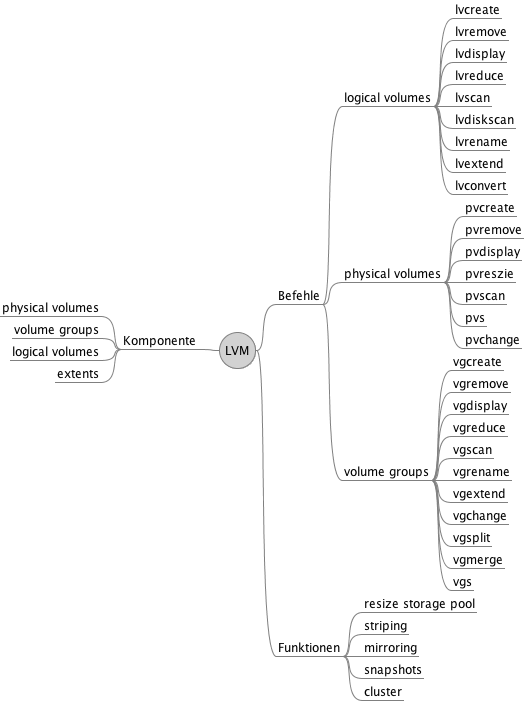
\includegraphics[width=0.75\textwidth]{LVMMindMap.png}
\caption{LVM: Mind Map}
\label{fig:LVMMindMap}
\end{figure}


\subsubsection{Physical Volumes (PV)}
Die unterste Schicht eines LVM Logical Volume ist eine physische Disk. Meist ist diese eine Festplatte, eine \gls{LUN}, welches über Storage Network \gls{SAN} zugeteilt wurde. Es kann aber auch nur eine Partition oder eine Datei sein, die als Disk verwendet wird. Eine physische Disk muss für die Verwendung im LVM als Physical Volume (PV) initialisiert werden. Dazu wird am Anfang der Disk ein entsprechender Label gesetzt, im Fachchargon auch "'labeling"' genannt.
Wie in Abbildung \myref{fig:PhysicalVolumeLayout} dargestellt, wird diese Kennzeichnung auch "'Label"' genannt, welches in den zweiten 512-Byte Sektor der Disk geschrieben wird. Dieses Kennzeichnung kann jedoch übersteuert werden, um den Label in einen der ersten Sektoren zu schreiben.

\begin{figure}[htb]
\centering
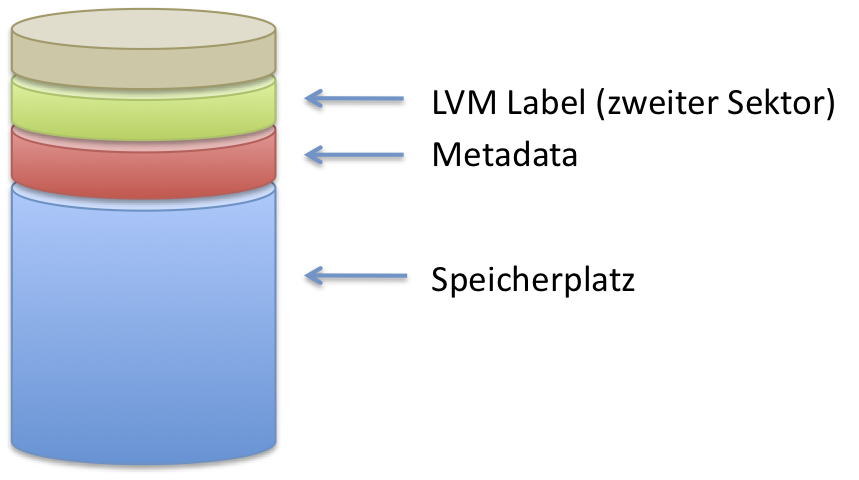
\includegraphics[width=0.8\textwidth]{PhysicalVolumeLayout.png}
\caption{Physical Volume: Layout}
\label{fig:PhysicalVolumeLayout}
\end{figure}

Der LVM Label dient dazu, die Disk korrekt zu identifizieren. Die Reihenfolge der Disk ist bei einen Neustart nicht gewährleistet, weshalb im Label ein eindeutiger zufälliger Identifikator bzw. eine Kennung, genannt "'UUID"', gespeichert wird. Anhand dieser UUID kann die Disk auch über einen Cluster wieder erkannt werden. 
Zusätzlich zur UUID sind im Label die Grösse der Disk in Bytes und die Record Adressen, in welche die LVM Metadata gespeichert sind, festgehalten.

Die LVM Metadaten enthalten die Konfigurationsdatei von LVM Volume Groups des Systems.

\subsubsection{Volume Group (VG)}\label{Volume Group (VG)}
Die Physical Volumes werden bei LVM zu Volume Groups kombiniert. Die erstellten Volume Groups dienen als Pool von Diskdpeicherplatz, welche zu Logical Volumes alloziert werden können. 
Beim Erstellen eines Volume Group aus ein oder mehreren Physical Volumes wird der Diskspeicherplatz des Physical Volumes in Einheiten bestehend aus einer fixen Grösse unterteilt, die sogenannten Physical Extents (PE).
Extents sind die kleinste physikalische Speichereinheit in einem LVM System. Die Extentsgrösse kann beim Erstellen des Volume Group gestgelegt werden, oder den Standardwert von 4 Megabyte übernommen werden. Die maximale Grösse eines Extent ist 1 Gigabyte. Die Anzahl an Extents in einer Volume Group ergibt sich aus der Summe aller Physical Volumes in einer Volume Group. Extents dienen zur "'n to m"' (Physical-to-Logical) Volumenzuordnung. Mehr dazu wird im Abschnitt \myref{Logical Volumes (LV)} erläutert.

\begin{figure}[htb]
\centering
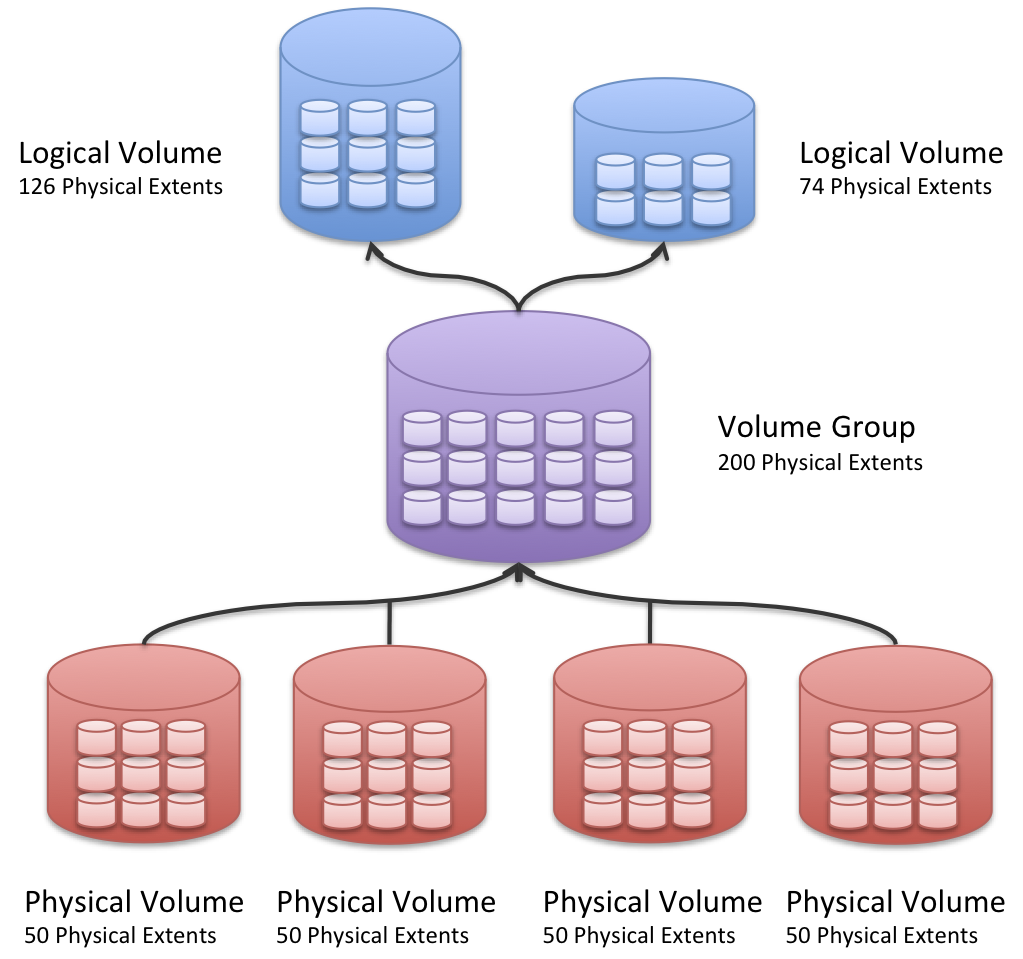
\includegraphics[width=1\textwidth]{ExtentsMapping.png}
\caption{Extents Mapping: Layout}
\label{fig:ExtentsMappingLayout}
\end{figure}

\subsubsection{Logical Volumes (LV)}\label{Logical Volumes (LV)}
Wie bereits beschrieben werden Logical Volumes aus einer Volume Group erstellt. Eine Volume Group kann in mehrere Logical Volumes unterteilt werden, jedoch kann sich ein Logical Volume nicht über mehrere Volume Groups erstrecken.
Wie im Abschnitt Volume Groups erwähnt, dienen Extents zum Zuordnen von Physical-to-Logical Volumes. Ein solches Mapping wird in Abbildung \myref{fig:ExtentsMappingLayout} veranschaulicht.
Eine Logical Volume wird analog zum Physical Volume in Extents unterteilt, sogenannte Logical Extents (LE).
Die Logical Extents besitzen die gleiche Grösse wie die Physical Extents der Volume Groups, in welcher sich das Logical Volume befindet. Die Grösse des Logical Volume setzt sich aus den Anzahl Physical Extents zusammen, welche aus der Volume Groups hinzugefügt wurde. Wird beim Erstellen der Volume Groups eine Extentgrösse von 32 Megabyte gewählt, kann die Logical Volume Grösse nur eine Vielfaches von 32 Megabyte sein. Ein Volume kann auf einen 64bit maximal 8 Exabytes gross sein. 

Die Abbildung \myref{fig:ExtentsMappingLayout} zeigt eine LVM Beispielkonfiguration. In diesem Beispiel wurden 4 Physical Volume mit je 50 Extents einer Volume Group zugeordnet. Somit verfügt die Volume Group über 200 Extents (4x50), welche sie ihren Logical Volumes zur Verfügung stellen kann. Aus diesen 200 Extents wurden in diesen Beispiel zwei Logical Volumes mit 126 Extents und 74 Extents erstellt. 

\paragraph{Flexible Kapazität} $\;$\\
Bei traditionellen Volumes kann ein Volume maximal die Grösse eines physischen Disks annehmen. Ein Logical Volume hingegen kann durch die Abstraktion fast beliebig vergrössert werden.
Durch die Zuordnung von weiteren Extents, welche in der Volume Group als "'frei"' makiert sind, kann das Logical Volume vergrössert werden. Wächst der Speicherplatz eines der beiden Logical Volumes gemäss Abbildung  \myref{fig:ExtentsMappingLayout}, müsste die Volume Group mit einer oder mehreren zusätzlichen Physical Volume ergänzt werden, um der Logical Volumes mehr Extents zuordnen zu können.

Umgekehrt kann das Logical Volume durch das Entfernen von Extents verkleinert werden. Sind in der Volume Group keine freien Extents mehr verfügbar, kann die Volume Group durch Zuordnung von weiteren Physical Volume vergrössert werden, welche wiederum einer Logical Volume Group zugeordnet werden kann.
Die kleinstmöglichste Wachstumgrösse der Logical Volume ist eine Extentsgrösse. Mehr zur Extentsgrösse wird im Abschnitt \myref{Volume Group (VG)} erklärt. 

\paragraph{Unterbruchsfreie Umplatzierung der Daten} $\;$\\
Durch LVM können die Logical Volumes inkl. Dateisystem und deren Daten zur Laufzeit auf neuere, performantere Speichersysteme umplatziert werden, ohne deswegen den Betrieb unterbrechen zu müssen. Trotz Verwendung der Disks ist es möglich, die Daten im Volume neu zu organisieren. Somit ist es kein Problem, eine verwendete physische Disk von Daten zu befreien, bevor diese ersetzt bzw. entfernt wird (z. B. bei der Renovation der physischen Umgebung).


\paragraph{Striping Volume} $\;$\\
Bei hoher Anzahl von sequenziellen schreib und lese zugriffe auf eine Volume ist es empfehlenswert eine Strips Volume zu verwenden. Striped Volumes 


\paragraph{Spiegelung von Volumes (Mirroring)} $\;$\\
Mirrored Logical Volumes sind exakte Kopien eines Volumes, welche durch Spiegelung, auch Mirroring genannt, dauernd mit dem Original in Synchronisation gehalten werden.
Wenn bei einem LVM für ein Volume eine Mirrored Logical Volume erstellt wird, stellt LVM sicher, dass wenn Daten auf ein darunter liegendes Physical Volume geschrieben werden soll, die Daten automatisch auf ein weiteres Physical Volume gespiegelt werden. LVM unterstützt zudem das Spiegeln auf mehrere Mirrored Volume. Durch die redundante Speicherung der Daten auf verschiedene Physical Volumes, werden die Daten und das System von Diskfehler besser geschützt. Tritt der Fall eines physischen Diskdefekt ein, steht zwar dieses Laufwerk dem System nicht mehr zur Verfügung, erlaubt aber dem System ohne Unterbruch mit den zusätzlichen Mirrored Volumes weiterzuarbeiten.
Für das Mirroring wird das Physical Volume in Regionen unterteilt, der Standardwert für die Region-Grösse ist 512 KB, zusätzlich wird ein kleines Log geführt, um nachzuvollziehen, welche Regionen deckungsgleich mit dem Original sind. Das Log wird zumeist aus Sicherheitsgründen auf eine weitere Disk bzw. Volume abgelegt. Manchmal wird es im Memory geführt, was aber bei einem Systemabsturz gefährliche Nachteile in sich birgt.

\begin{figure}[H]
\centering
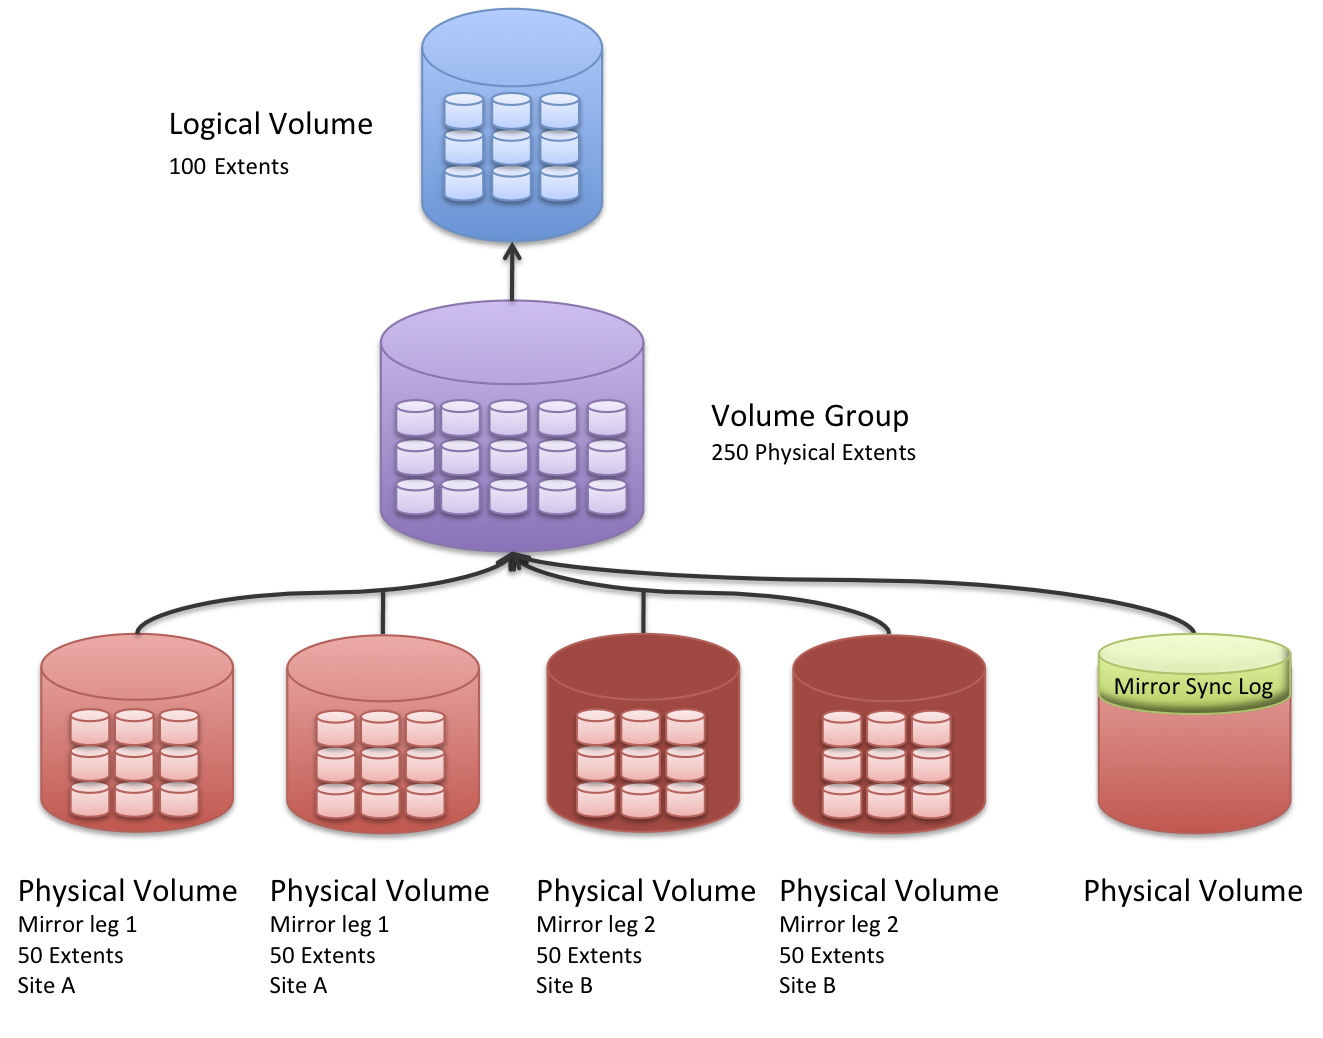
\includegraphics[width=1\textwidth]{LVMMirrorArchitectur.png}
\caption{LVM: Mirror Architektur}
\label{fig:LVM Mirror Architektur}
\end{figure}

Mirroring wird in den meisten Fällen nicht als Ersatz eines RAID-1 Systeme betrachtet. In vielen Modernen IT-Landschaften werden die Disk bzw. \gls{LUN} über eine Storage Area Network (\gls{SAN}) einem System zur Verfügung gestellt. Diese \gls{LUN} stammen meist aus einer RAID-1 oder RAID-5 Diskgruppe und sind somit im Storage System redundand. Das Mirroring wird in solchen Fällen meist zur Spiegelung der Daten in ein weiteres Rechenzentrum angewendet. Indem das LVM mehrere mirrored Disks unterstützt, können die Daten in mehrere Rechenzentren gespiegelt werden. 


Die Abbildung \myref{fig:LVM Mirror Architektur} zeigt eine mögliche Architektur eines LVM Mirrors, welche über zwei Rechenzentren Site A und Site B gespiegelt wird. Dazu wurden je zwei Physical Volume über jeweils eine Network Storage System pro Rechenzentrum zugeordnet. Das Mirror Log wird auf eine separaten Physical Volume geschrieben. Mit dieser Architektur lassen sich in Cluster Umgebungen hoch redundante Systeme bauen.


\paragraph{Snapshot} $\;$\\
LVM unterstützt das Erstellen von \gls{Snapshot}s eines Logical Volume. Wenn ein \gls{Snapshot} erstellt wurde, werden alle Änderungen im Volume im \gls{Snapshot} gespeichert und das Original Volume bleibt unverändert im Originalzustand. Beim Erstellen eines \gls{Snapshot} ist darauf zu achten, dass die Snapshot-Grösse etwas mehr Speicherplatz zur Verfügung steht, als die geplante Änderung benötigt. Sobald der reservierte Speicherplatz eines \gls{Snapshot} voll ausgenutzt wurde, können neue Änderungen nicht mehr nachvollzogen bzw. gespeichert werden, wodurch das \gls{Snapshot} ungültig wird und alle Änderungen verloren gehen.
Um ein "'Überlaufen"' zu verhindern, sollten \gls{Snapshot} regelmässig und zeitnah überwacht werden und bei Bedarf genügend vergrössert werden.

Snapshots bieten beim Betrieb eines Systems einige Vorteile:

\begin{figure}[htb]
\centering
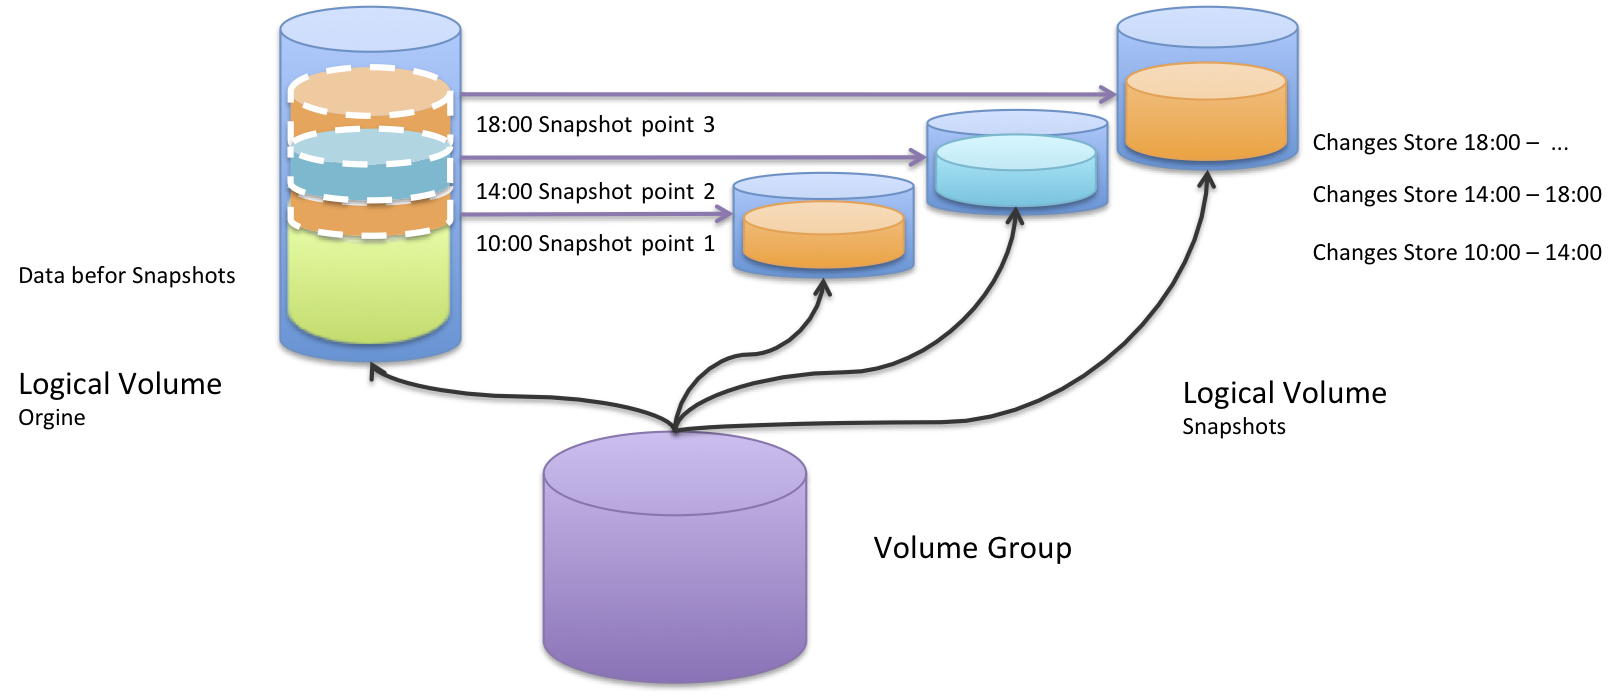
\includegraphics[width=1.2\textwidth]{LVMSnapshot2.png}
\caption{LVM: Snapshot}
\label{fig:LVMSnapshot}
\end{figure}


\begin{itemize}
\item Es können Tests gegen produktive Daten durchgeführt werden
\item Sollen z.B. Datenbanken während des laufenden Betriebes gesichert werden, können mit Hilfe der LVM \gls{Snapshot} Technologie die Daten parallel gesichert werden, auch wenn zur gleichen Zeit die Originaldaten (zu sichernde Daten) sich verändern sollten (erhalten der Datenkonsistenz).
\item Ein File-Systemcheck kann mit Hilfe der LVM Technologie auf dem Filesystem getestet werden.
\end{itemize}

\paragraph{Clustered Logical Volume Manager} $\;$\\
Clustered Logical Volume Manager (CLVM) ermöglicht es, wie im Abschnitt "'Entstehung LVM"' erwähnt, die Verwendung von LVM im \gls{Cluster} Umfeld. CLVM besteht aus dem Deamon clvmd welche auf allen \gls{ClusterNode}s installiert und während des Bootvorgangs gestartet sein müssen. Bei einer Änderung an der Volume Konfiguration verteilt der Deamon clvmd die aktuellen LVM Metadaten an alle Nodes und ermöglicht damit, dass alle Nodes dieselbe Sicht auf die Logical Volumes haben. In der Konfigurations Datei  lvm.conf von LVM muss für CLVM der Locking Typ der Volumes auf Typ 3 "'Built-in clustered locking"' angepasst werden.


\section{Einarbeiten in LVM (LVM2 Commands)}

\subsection{Physical Volume anlegen}

Mit folgendem Beispielbefehl werden aus einem Block-Laufwerk \textit{/dev/sdb}, \textit{/dev/sdc}, \textit{/dev/sdd} und \textit{/dev/sde} vier Physical Volumes erstellt und gelabelt.  

\Shell{pvcreate /dev/sdb /dev/sdc /dev/sdd /dev/sde}


Mehr Informationen sind in den MAN Pages\footnote{\href{http://linux.die.net/man/8/pvcreate}{http://linux.die.net/man/8/pvcreate}}  zu finden.

\subsection{Physical Volume entfernen}

Mit dem Befehl  \textbf{pvremove} kann ein Physical Volume Label auf aus einem Block-Laufwerk entfernt werden.

\Shell{pvremove /dev/sdb}


Mehr Informationen sind in den MAN Pages\footnote{\href{http://linux.die.net/man/8/pvcreate}{http://linux.die.net/man/8/pvcreate}}  zu finden.

\subsubsection{Volume Group anlegen}

Mit dem Befehl vgcreate kann man aus einem oder mehreren Physical Volumes eine Volume Group erstellen. Die Extentsgrösse kann mit der Option \textbf{-s} bestimmt werden. Wird diese Option nicht genutzt, so verwendet das LVM die Standardgrösse, welche in der lvm.conf festgelegt ist. Die Extentgrösse von 32 MB hat sich in der Praxis bewährt.
Grössere Extents haben keinen Einfluss auf eine verbesserte I/O Performance.
Die Zuordnung der Physical Extents, kann mit \textbf{--alloc} definiert werden. Die Standardkonfiguration \textbf{normanl} muss nur in speziellen Fällen angepasst werden, wenn aus speziellen Performancegründen evtl. beim Backup parallele Strips gewünscht wird.

\Shell{vgcreate VolGroupData}

Volume Groups in einer Cluster-Umgebung, welche mit CLVM auf einem geteilten Storage erstellt wurden, sind von allen Cluster Nodes sichtbar. Mit der Option \textbf{-c} wird die Sichtbarkeit der Volume Group auf den lokalen Node beschränkt.

\Shell{vgcreate -c VolGroupCluData1 /dev/sdb /dev/sdc /dev/sdd /dev/sde}


Mehr Informationen sind in den MAN Pages\footnote{\href{http://linux.die.net/man/8/vgcreate}{http://linux.die.net/man/8/vgcreate}} zu finden.

\subsubsection{Konfiguration von Volume Group auslesen}

Mit dem Befehl \textbf{vgdisplay} \textbf{vgs} kann die Konfiguration der Volume Group ausgelesen werden.
Der Befehl \textbf{vgdisplay} eignet sich um eine schnelle Übersicht zu gewinnen. Der Befehl \textbf{vgs} eignet zum Auslesen der Konfiguration per Script, da mit Optionen die Ausgabe individuell angepasst werden kann.

\Shell{vgdisplay VolGroupCluData1}

\Shell{vgs}


Mehr Informationen sind in den MAN Pages\footnote{\href{http://linux.die.net/man/8/vgdisplay}{http://linux.die.net/man/8/vgdisplay}} \footnote{\href{http://linux.die.net/man/8/vgs}{http://linux.die.net/man/8/vgs}} zu finden.

\subsubsection{Konfiguration von Volume Group anpassen}

Mit dem Befehl \textbf{vgchange} kann die Konfiguration einer bestehende Volume Group angepasst werden.


Mehr Informationen sind in den MAN Pages\footnote{\href{http://linux.die.net/man/8/vgchange}{http://linux.die.net/man/8/vgchange}} zu finden.

\subsubsection{Volume Group vergrössern}

Durch Hinzufügen von weiteren Physical Volumes kann eine Volume Group vergrössert werden und somit Speicherplatz für weitere Logical Volumes oder vergrösserte Logical Volumes zur Verfügung gestellt werden.

\Shell{vgextent VolGroupCluData1  /dev/sdf /dev/sdg }


Mehr Informationen sind in den MAN Pages\footnote{\href{http://linux.die.net/man/8/vgextent}{http://linux.die.net/man/8/vgextent}} zu finden.

\subsubsection{Volume Group entfernen}

Sind alle Logical Volumes einer Volume Group entfernt worden, kann mit dem Befehl \textbf{vgremove} die Volume Group vom System entfernt werden. Die Eigenschaft "'Cur LV"' der Ausgabe von \textbf{vgdisplay} zeigt die Anzahl Logical Volumes der Volume Groupe und sollte vor dem Entfernen der Volume Group 0 stehen.

\Shell{vgremove VolGroupCluData1}

Mehr Informationen sind in den MAN Pages\footnote{\href{http://linux.die.net/man/8/vgremove}{http://linux.die.net/man/8/vgremove}} zu finden.

\subsubsection{Logical Volume anlegen}

Mit dem Befehl \textbf{lvcreate}  können lineare, striped oder mirrored Volumes angelegt werden.
Grundvoraussetzung für das Anlegen eines Logical Volumes ist, dass auf dem System bereits mindestens eine Volume Group angelegt wurde.

In diesen Beispiel wird eine Logical Volume mit der Grösse von 2 GB auf der Volume Groupe VolClusterData1 angelegt. 

\Shell{lvcreate -L 2G VolClusterData1}

Wird kein Namen für das Logical Volume mit der Option \textbf{-n lvname} festgelegt, vergibt LVM automatisch einen generierten Namen "'lvol0"' (dieser wird durchnummeriert).

\Shell{lvcreate -L 2G VolClusterData1 -n clvdata1}

Die Grösse eines LVM kann auch prozentual zur Volume Group Grösse mit dem Zusatz \textbf{VG} definiert werden oder prozentual zum restlichen freien Speicherplatz der Volume Group mit dem Zusatz \textbf{FREE}.

\Shell{lvcreate -L 50\%VG VolClusterData1 -n clvdata1}

\Shell{lvcreate -L 50\%FREE VolClusterData1 -n clvdata1}

Mehr Informationen sind in den MAN Pages\footnote{\href{http://linux.die.net/man/8/lvcreate}{http://linux.die.net/man/8/lvcreate}}  zu finden.

\subsubsection{Striped Locical Volume anlegen}

Eine Striped Logical Volume wird mit \textbf{lvcreate} und der Option \textbf{-i} und der Anzahl an Physical Volumes aus der Volume Group angelegt, welche für LVM verwendet werden soll. Die Grösse eines einzelnen Strips kann mit der Option \textbf{-I} festgelegt werden. In der Praxis haben sich Stripgrössen von 64kB oder 128kB bewährt.

\Shell{lvcreate -L 2G  -i2 -I64 VolClusterData1 -n clvdata1}

\subsubsection{Mirrored Locical Volume anlegen}

Eine Mirrored Logical Volume wird mit der Option \textbf{-m} plus der Anzahl der Mirrored Volumes angelegt. Das unten aufgeführte Beispiel legt zwei Mirrored Volumes an und legt somit fest, dass die Daten dreifach gespeichert werden sollen.

\Shell{lvcreate -L 2G -m2 VolClusterData1 -n clvdata1}


\subsubsection{Logical Volume grösse anpassen}

Wird mehr Speicherplatz im Logical Volume benötigt, kann der Speicherplatz mit dem Befehl \textbf{lvresize} 
angepasst werden. Bevor man das Logical Volume vergrössert, sollte man prüfen, ob die darunter liegende Volume Groupe noch genügen freie Extents hat.

\Shell{lvextend -L +2G /dev/VolGroupCluData1/VolClusterData1 }

Eine Logical Volume kann auf dieselbe Weise auch wieder verkleinert werden. Hier ist darauf zu achten, dass man das darüber liegende Filessystem vorher verkleinert hat.

\Shell{lvextend -L -1G /dev/VolGroupCluData1/VolClusterData1 }

Mehr Informationen sind in den MAN Pages\footnote{\href{http://linux.die.net/man/8/lvextend}{http://linux.die.net/man/8/lvextend}} zu finden.

\subsubsection{Logical Volume entfernen}

Wird das Logical Volume nicht mehr benötigt, kann das Logical Volume mit dem Befehl \textbf{lvremove} 
entfernt werden. Die Verwendeten Extents des Logical Volume werden in der Volume Group als frei markiert. Achtung alle Daten auf dem Volume gehen verloren. 

\Shell{lvremove /dev/VolGroupCluData1/VolClusterData1 }

Mehr Informationen sind in den MAN Pages\footnote{\href{http://linux.die.net/man/8/lvremove}{http://linux.die.net/man/8/lvremove}} zu finden.

\chapter{Analyse}
\label{cha:Analyse}


\section{Anforderungsanalyse}
Für die Anforderungsanalyse wurde aufgrund der Projekt- und Applikationsgrösse das User-Stories Verfahren gewählt. Für die Ausarbeitung der Anforderungen wurde ein kleines Gremium zusammengestellt, welche die einzelnen Interessengruppen vertreten. Zu den Intressengruppen gehören der Teamleiter, die Storage Admins, die Capacity Planer und der System Admin und System Engineer. 
Die Use Cases wurden anschliessend in zwingende Anforderungen und nicht-zwingende Anforderungen unterteilt.

\textbf{Lukas (System Engineer):}

\fbox{\parbox{\linewidth}{Mit dem Tool vorgenommene Änderungen müssen aufgezeichnet (geloggt) werden.}}

\fbox{\parbox{\linewidth}{Bevor die Änderungen vorgenommen werden, soll eine Zusammenfassung angezeigt werden (idealierweise mit graphischer Darstellung)}}\newline\newline

 
\textbf{Thorsten (Storage Admin):}

\fbox{\parbox{\linewidth}{Als Storage Admin kann ich den Storage End-to-End bis zum Filesystem bereitstellen}}

\fbox{\parbox{\linewidth}{Als Capacity Planer kann ich mir schnell und einfach einen Überblick über den benutzten und verfügbaren Diskspace verschaffen}}

\fbox{\parbox{\linewidth}{Als User kann ich einfach neuen Diskspace auf meinem Server bestellen und kann den Workflow verfolgen.}}\newline\newline


\textbf{Daniel (System Admin):}

\fbox{\parbox{\linewidth}{Als System Admin kann ich das Volumes des Servers vergrössern, ohne LVM Befehle kennen zu müssen}}

\fbox{\parbox{\linewidth}{Als System Admin kann ich beim Vergrössern der Volumes automatisch das Filesystem vergrössern}}

\fbox{\parbox{\linewidth}{Als System Admin kann ich ein Site-übergreifendes Mirroring einrichten}}

\fbox{\parbox{\linewidth}{Als System Admin kann ich den Diskspace auf ein anderes Storage System migrieren }}

\fbox{\parbox{\linewidth}{Als System Admin werde ich beim sicheren Entfernen eines Disk eines gewählten Servers von der Anwendung unterstützt }}

\fbox{\parbox{\linewidth}{Als System Admin erhalte ich einen raschen Überblick über die Diskkonfiguration des zu wartenden Servers}}\newline\newline

\textbf{David (Teamleiter):}

\fbox{\parbox{\linewidth}{Als Teamleiter kann ich nachvollziehen wer, wann welche Änderung vorgenommen hat}}

\fbox{\parbox{\linewidth}{Als Applikation Owner kann ich den zugewiesenen Diskplatz prüfen}}

\textbf{Philipp (Capacity Admin):}

\fbox{\parbox{\linewidth}{Als Capacity Planer kann ich eine Storagereservation vornehmen }}

\fbox{\parbox{\linewidth}{Als Capacity Planer erhalte ich einen raschen Überblick auf die noch unbenutzten Storages }}


\subsection{Zwingend}

Die folgenden Anforderungen müssen zwingend umgesetzt werden:

\begin{itemize}
\item Als System Admin kann ich das Filesystem des Server vergrössern, ohne LVM Befehle zu kennen
\item Als System Admin kann ich Storage am Server wieder reduzieren
\item Als System Admin erhalte ich einen raschen Überblick über die Diskkonfiguration des Servers
\item Als User kann ich einfach neuen Diskspace auf meinem Server bestellen und kann den Workflow verfolgen.
\item Die dem vom Tool vorgenommenen Änderungen müssen aufgezeichnet (geloggt) werden.
\end{itemize}

\subsection{Nicht zwingend}

Die folgenden Anforderungen, werden in diesem Projekt nicht umgesetzt, auch wenn einige davon für eine Produktiveversion interessante und wichtige Anforderungen wären:

\begin{itemize}
\item Als Capacity Planer kann ich Storage reservieren
\item Als Applikation Owner kann ich den zugewiesenen Diskplatz prüfen
\item Als Capacity Planer kann ich mir schnell und einfach einen Überblick über den benutzten und verfügbaren Diskspace verschaffen
\item Bevor die Änderungen vorgenommen werden, soll eine Zusammenfassung (idealerweise graphisch dargestellt) angezeigt werden
\end{itemize}


\section{Marktanalyse}
\subsection{Potenzielle Kunden}
Unternehmen konkurrenzieren sich nicht nur im Produkteverkauf und bei der Aquisition von neuen Kunden, sonder auch bei der effizienten Gestaltung der internen Abläufe und optimalen Nutzung der eigenen Ressourcen. Seit Beginn des Computerzeitalters hat die Bedeutung der IT in ausnahmslos allen Unternehmen stark zugenommen. Unternehmen mit einer schlecht funktionierenden IT-Infrastruktur verlieren am Markt an Konkurrenzstärke und manövrieren sich über kurz oder lang auf das Abstellgeleise mit einer unsicheren Zukunft. Eine moderne Geschäftsleitung hat dies längst erkannt und legt Wert auf die Erhaltung und den Ausbau der inneren Stärke in Bezug auf die Abstimmung der Business-Strategie mit der Leistung der IT. Was nützt der beste Verkäufer, wenn es nach dem Verkaufsabschluss mit der Umsetzung des Auftrages happert.

Die Autoren \Autor{4755749} haben in einem Artikel über das Thema IEEE, die Frage der CIO-Charakteristik zur Unternehmensstrategie untersucht:

\begin{quote}
"''In a diverse, ever-changing marketplace, organizations are constantly seeking to harness technology to improve their core competency and gain competitive advantage. \textbf{Explicitly, knowing how to apply Information Systems (IS) in an appropriate and timely way and in harmony with business strategies, goals, and needs could bring the organization to steps closer to business success.} In other words, aligning IS strategy to business strategy becomes a critical issue in most organizations. Indeed, there is an increasing amount of research and understanding on the linkages between business and IS strategies, the role of partnerships between IS and business management, and the need to understand the transformation of business strategies resulting from the competitive use of IS."'' \footnote{\Zitat[S.~1]{4755749}}
\end{quote}


Trotz der zunehmenden Bedeutung der IT-Leistung für die innerbetrieblichen Abläufe aber auch vermehrt direkt an der Verkaufsfront, steigt der Druck an stetiger Optimierung und effizienteren Verarbeitung der IT-Prozesse in den IT-Abteilungen. Zusätzlicher Druck von Aussen bezüglich politischen und marktwirtschaftlichen Veränderungen, ich denke da zB. an neue Gesetze und Regulatorien, erhöht die Erwartungen an die IT Dienstleistung.
Unternehmen vergleichen sich heute immer mehr an der Leistungsfähigkeit ihrer IT-Leistung wie zB. bezüglich der Kostenstruktur oder Funktionalität mit der Konkurrenz. Schneidet die Effizienz der IT-Abteilung (Leistung versus Kosten) schlecht ab, sind die Gegenmassnahmen oft drastisch und erfordert höchste Konzentration des IT-Managements. Zu nennen sind da unter anderem massive Kosteneinsparungen, Streichung oder Aufschiebung von Projekten, Entlassung von internen und externen Mitarbeiter, Outsourcing bzw. Insourcing, um nur einige der möglichen Massnahmen aufzuführen. Dass solche Eingriffe  den IT-Betrieb zusätzlich lähmen kann versteht sich von selbst. Eine laufende Überprüfung und Verbesserung der eigenen Organisation und Kostenstruktur gehört zum Tagesgeschäft des erfolgreichen IT-Managers. Es verwundert nicht, dass daraus auch neue Modell entstehen, wie zB. das anbieten der IT-Dienstleistung als Profit-Center innerhalb des Gesamtbetriebes, die Auslagerung der Dienste ins Ausland nach dem Outsourcing Modell der Inder oder die Aufsplittung der Services in Production und Engineering. In diesem Sinn ist dieses Projekt zu verstehen, indem eben die Storage-Verwaltung vereinfacht und effizienter gestaltet werden soll, um damit einen vielleicht kleinen, aber wichtigen Beitrag zur Verringerung der IT-Kosten zu erfüllen. 


\subsection{Server Markt}
\subsubsection{Betriebsystem}
Waren vor ein paar Jahren Linux-Installationen im Server-Bereich, meist als ideologisch und experimentell angesehen, hat sich dies in der Zwischenzeit gewandelt.
Vermehrt wird Linux für Hosting- und Web-Installationen in Klein- bis Grossbetrieben professionell eingesetzt und hat Boden gegenüber von dominierenden Windows-Server-Installationen gutgemacht. Dank zunehmender Unterstützung seitens Software Herstellern für die Linux-Plattform steigt das Interesse an Linux im professionellen Geschäftsumfeld. Vergleicht man das Angebot der Betriebsystem Hersteller Oracle, IBM und Microsoft mit dem Angebot der beiden Linux Distributoren Red Hat und Novell Suse, ist ersichtlich, dass sich die Angebote bezüglich Wartung, Support und Dienstleistungen nicht wesentlich voneinander unterscheiden. 
Trotz diesem heute breiten Angebot an Funktionalität im Linux Umfeld, konnte sich dieses Betriebsystem bis anhin im Finanzdienstleistungs-Branche bei den Unternehmen nicht durchsetzen, ausser für dedizierte Web-Installationen. Traditionell dominieren in diesem Marktsegment immer noch die Betriebsysteme wie Windows, Oracle Solaris (SUN) bzw. IBM AIX als die strategisch geführten Plattformen. Es gibt jedoch Anzeichen, dass sich dieses Verhältnis künftig ändern könnte, denn einige Unternehmen haben für neue Projekte ein Auge auf Linux neben Windows geworfen und liebäugeln Linux nun auch als strategische  Betriebsystem Plattform einzusetzen.

\subsubsection{Hardware Platform}
\begin{figure}[htb]
\centering
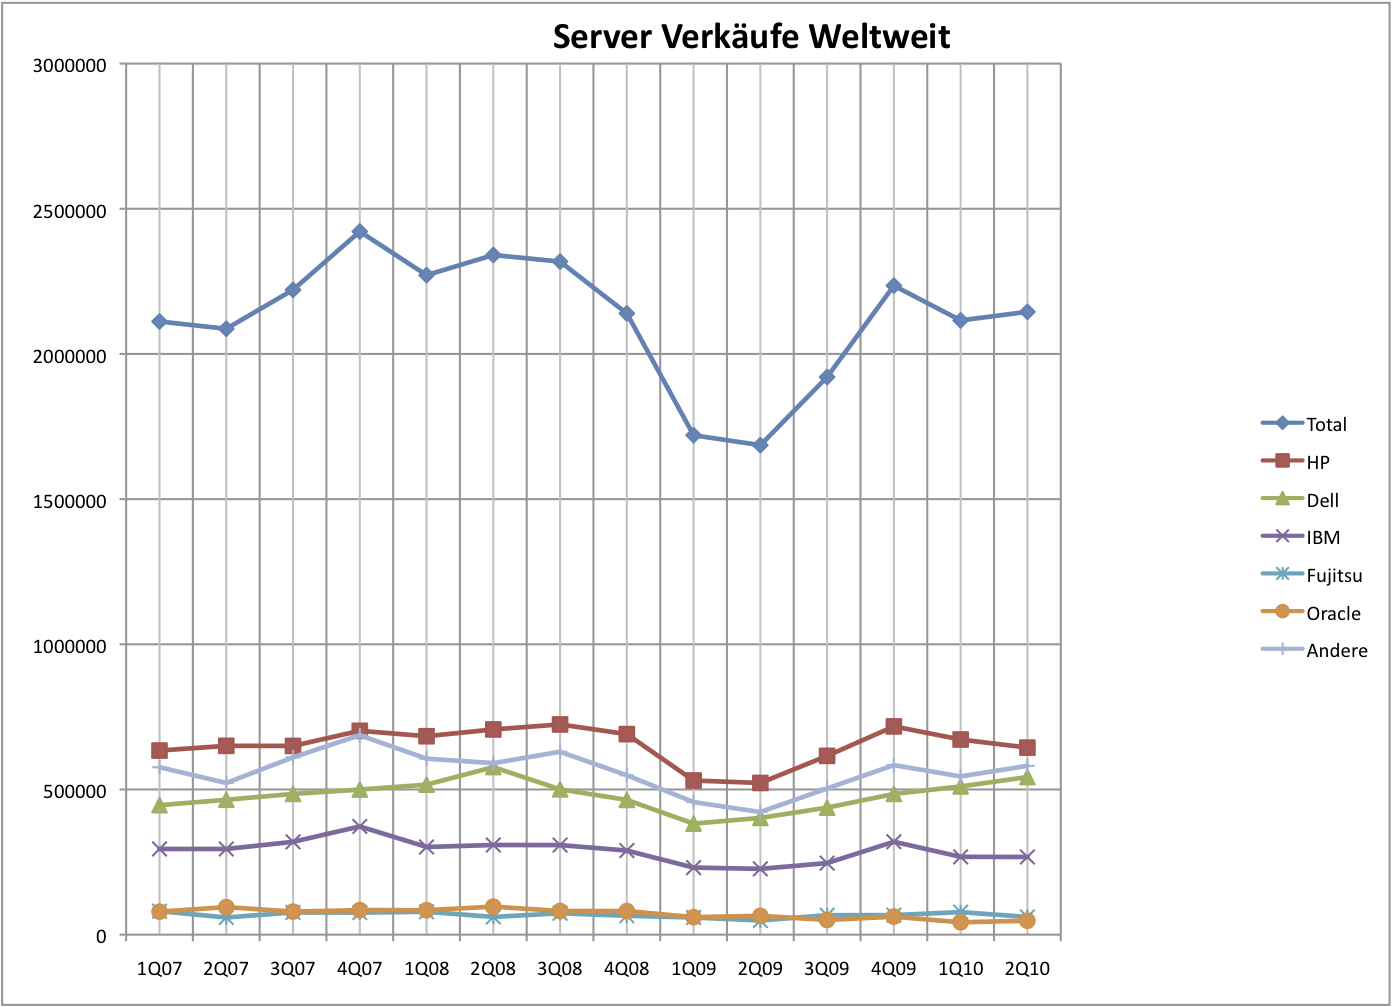
\includegraphics[width=1\textwidth]{DiagrammServerVerkaufeWeltweitQuartal.png}
\caption{Diagramm - Server Verkauf: Weltweit pro Quartal \textit{Quelle Gartner}}
\label{fig:DiagrammServerVerkaufeWeltweitQuartal}
\end{figure}

Ein möglicher Faktor für die zunehmende Ablösung der Betriebsysteme Solaris und AIX durch Linux könnte deren Hardware Plattform, welche zumeist auf RISC bzw. Intanium Prozessoren basieren, sein. 
Im Low- und Midrange Bereich sind solche Hardware Systeme nicht gleich Leistungsfähig wie Systeme welche auf den x86 bzw. die x64 Prozessor-Architektur aufgebaut sind. Zudem lassen die höheren Kosten für den Betrieb und Unterhalt von zwei unterschiedlichen Hardware-Plattformen innerhalb deselben Unternehmens solche Projekte verständlicherweise in den Hintergrund drängen.
Diese Einschätzung decken sich auch mit der Server-Hardware Marktanteil Analyse vom zweiten Quartal 2010 von Gartner. Die x86 basierenden Systeme sind um 28.9 Prozent in der verkauften Stückzahl und in 37 Prozent im Umsatz gewachsen. RISC/Itanium basierenden Systeme haben im gleichen Zeitraum  im Vergleich zum selben Vorjahresquartal 16.5 Prozent bezüglich der verkauften Stückzahlen sowie 8.8 Prozent beim Umsatz verloren.

Das Linien-Diagramm der \abbildung{DiagrammServerVerkaufeWeltweitQuartal} zeigt die Anzahl verkauften Servern der einzelnen Herstellern vom ersten Quartal 2007 bis zum zweiten Quartal 2010. 
Aus dem Diagramm kann man nicht direkt erkennen, dass die x86/x64 Prozessor-Architektur bei den Servern im Vergleich zu RISC bzw. Itanium Prozessoren überwiegt. Neben HP und Dell, welche hauptsächlich x86/X64 Server verkaufen, ist Oracle einer der führenden RISC Server Hersteller bezüglich der Anzahl verkaufter Server weit abgeschlagen. Zudem kann man aus den \tabelle{WeltServerWarenlieferung2010} und \tabelle{EMEAServerWarenlieferung2010} erkennen, dass Oracle im zweiten Quartal 2010 gegenüber der Konkurrenz den stärksten Abastzrückgang erleiden musste.

Gemäss Herrn O'Connell von Garnter sind die Rückgänge vom RISC/Itanium Segment auf die folgenden Ursachen rückzuführen:

\begin{quote}
“'The first half of 2010 has seen continued challenges for vendors in the server segment of RISC and Itanium Unix. The combination of longer sales cycles for these systems, product refreshes and ongoing economic uncertainty has resulted in RISC/Itanium Unix revenue in the second quarter of 2010 being less than half that of the second quarter of 2008, we expect this market to improve in the second half of 2010, but vendors in this segment will face an increasingly difficult challenge in minimizing migrations to Windows and Linux platforms.”'
\footnote{O’Connell, http://www.gartner.com/it/page.jsp?id=1426834}
\end{quote}

Wie man in der Tabelle \ref{tab:WeltServerWarenlieferung2010} von Gartner über die weltweiten Server Warenlieferungen im zweiten Quartal 2010 erkennen kann, haben die beiden grössten Server Hersteller mit RISC Architektur eine Wachstumsverlangsamung gegenüber dem gleichen Quartal 2009 in Kauf nehmen müssen. Die restlichen Hersteller hatten ein der selben Periode ein positives Wachstum verzeichnet. Bei IBM ist diese Zahl wenig aussagefähig, da nicht hervorgeht wie der Rückgang der Zahlen auf die Produkte bezüglich Prozessor Architektur aufzuteilen sind.


\begin{longtable}{|m{1,7cm}|m{2,3cm}|m{1,4cm}|m{2,2cm}|m{1,4cm}|m{1,3cm}m{0.01mm}|}
\caption{ Weltweite: Hersteller Server Warenlieferung Q2 2010 (Stück)} \\
\hline
\label{tab:WeltServerWarenlieferung2010}
& Q2 10 &  Q2 10 & Q2 09 & Q2 09 & Q2 09 - Q2 10 & \\
\textbf{Hersteller}& \textbf{Stückzahl}& \textbf{Markt- Anteil}& \textbf{Stückzahl}& \textbf{Markt- Anteil} &\textbf{Wach- stum}&\\
\hline
HP & \raggedleft 644'172 &\raggedleft  30,0 \% & \raggedleft 522'447 & \raggedleft 31,0 \% &  \raggedleft 23,3 \% & \\
\hline
Dell & \raggedleft 542'799 & \raggedleft 25,3 \% & \raggedleft 402'187 & \raggedleft 23,8 \% &\raggedleft 35,0 \%& \\
\hline
IBM & \raggedleft 267'614 & \raggedleft 12,5 \% & \raggedleft 226'570 & \raggedleft 13,4 \% & \raggedleft 18,1 \% &\\
\hline
Fujitsu &\raggedleft 60'974 &\raggedleft 2,8 \%  & \raggedleft 48'819 & \raggedleft 2,9 \% &  \raggedleft 24,9 \% &\\
\hline
Sun & \raggedleft 47'968 & \raggedleft 2,2 \%  & \raggedleft 64'810 & \raggedleft 3,8 \% & \raggedleft  -26,0 \% &\\
\hline
Andere Hersteller & \raggedleft 581'512 & \raggedleft 27,1 \%  & \raggedleft 422'371 & \raggedleft 37,7 \% &  \raggedleft 27,1 \%& \\
\hline
\hline
\textbf{Total} & \raggedleft 2'145'039 & \raggedleft 100,0 \%  &\raggedleft 1'687'204 & \raggedleft 100,0 \% &  \raggedleft 27,1 \% &\\
\hline
\end{longtable}


\begin{longtable}{|m{1,7cm}|m{2,3cm}|m{1,4cm}|m{2,2cm}|m{1,4cm}|m{1,3cm}m{0.01mm}|}
\caption{ Weltweite: Hersteller Server Warenlieferung Q2 2009 (Stück)} \\
\hline
\label{tab:WeltServerWarenlieferung2009}
& Q2 09 &  Q2 09 & Q2 08 & Q2 08 & Q2 08 - Q2 09 & \\
\textbf{Hersteller}& \textbf{Stückzahl}& \textbf{Markt- Anteil}& \textbf{Stückzahl}& \textbf{Markt- Anteil} &\textbf{Wach- stum}&\\
\hline
HP & \raggedleft 522'447 &\raggedleft  31,0 \% & \raggedleft 706'724 & \raggedleft 30,2 \% &  \raggedleft -26,1 \% & \\
\hline
Dell & \raggedleft 402'187 & \raggedleft 23,9 \% & \raggedleft 577'163 & \raggedleft 24,7 \% &\raggedleft -30,3 \%& \\
\hline
IBM & \raggedleft 226'570 & \raggedleft 13,4 \% & \raggedleft 308'835 & \raggedleft 13,2 \% & \raggedleft -26,6 \% &\\
\hline
Sun &\raggedleft 63'412 &\raggedleft 3,8 \%  & \raggedleft 96'510 & \raggedleft 4,1 \% &  \raggedleft -26,6 \% &\\
\hline
Fujitsu & \raggedleft 48'819 & \raggedleft 2,9 \%  & \raggedleft 61'077 & \raggedleft 2,6 \% & \raggedleft  -20,1 \% &\\
\hline
Andere Hersteller & \raggedleft 422'371 & \raggedleft 25,1 \%  & \raggedleft 590'468 & \raggedleft 25,2 \% &  \raggedleft -28,5 \%& \\
\hline
\hline
\textbf{Total} & \raggedleft 1'685'806 & \raggedleft 100,0 \%  &\raggedleft 1'687'204 & \raggedleft 100,0 \% &  \raggedleft -28,0 \% &\\
\hline
\end{longtable}


\begin{longtable}{|m{1,7cm}|m{2,3cm}|m{1,4cm}|m{2,2cm}|m{1,4cm}|m{1,3cm}m{0.01mm}|}
\caption{ EMEA: Server Hersteller Warenlieferung Q2 2010 (Stück)} \\
\hline
\label{tab:EMEAServerWarenlieferung2010}
& Q2 10 &  Q2 10 & Q2 09 & Q2 09 & Q2 09 - Q2 10 & \\
\textbf{Hersteller}& \textbf{Stückzahl}& \textbf{Markt- Anteil}& \textbf{Stückzahl}& \textbf{Markt- Anteil} &\textbf{Wach- stum}&\\
\hline
HP & \raggedleft 241'898 &\raggedleft  41,5 \% & \raggedleft 200'421 & \raggedleft 40,6 \% &  \raggedleft 20,7 \% & \\
\hline
Dell & \raggedleft 111'328 & \raggedleft 19,1 \% & \raggedleft 90'273 & \raggedleft 18,3 \% &\raggedleft 23,3 \%& \\
\hline
IBM & \raggedleft 63'701 & \raggedleft 10,9 \% & \raggedleft 62'359 & \raggedleft 12,6 \% & \raggedleft 2,2 \% &\\
\hline
Fujitsu &\raggedleft 36'575 &\raggedleft 6,3 \%  & \raggedleft 31'207 & \raggedleft 6,3 \% &  \raggedleft 17,2 \% &\\
\hline
Sun & \raggedleft 15'473 & \raggedleft 2,7 \%  & \raggedleft 24'053 & \raggedleft 4,9 \% & \raggedleft  -35,7 \% &\\
\hline
Andere Hersteller & \raggedleft 114'558 & \raggedleft 19,6 \%  & \raggedleft 84'743 & \raggedleft 17,2 \% &  \raggedleft 35,2 \%& \\
\hline
\hline
\textbf{Total} & \raggedleft 583'533 & \raggedleft 100,0 \%  &\raggedleft 492'056 & \raggedleft 100,0 \% &  \raggedleft 18,4 \% &\\
\hline
\end{longtable}

\begin{longtable}{|m{1,7cm}|m{2,3cm}|m{1,4cm}|m{2,2cm}|m{1,4cm}|m{1,3cm}m{0.01mm}|}
\caption{ EMEA: Hersteller Server Warenlieferung Q2 2009 (Stück)} \\
\hline
\label{tab:EMEA:ServerWarenlieferung2009}
& Q2 09 &  Q2 09 & Q2 08 & Q2 08 & Q2 08 - Q2 09 & \\
\textbf{Hersteller}& \textbf{Stückzahl}& \textbf{Markt- Anteil}& \textbf{Stückzahl}& \textbf{Markt- Anteil} &\textbf{Wach- stum}&\\
\hline
HP & \raggedleft 200'421 &\raggedleft  40,8 \% & \raggedleft 293'621 & \raggedleft 40,6 \% &  \raggedleft -31,7 \% & \\
\hline
Dell & \raggedleft 90'273 & \raggedleft 18,4 \% & \raggedleft 138'000 & \raggedleft 19,1 \% &\raggedleft -34,6 \%& \\
\hline
IBM & \raggedleft 62'359 & \raggedleft 12,7 \% & \raggedleft 95'861 & \raggedleft 13,3 \% & \raggedleft -34,9 \% &\\
\hline
Fujitsu &\raggedleft 31'207 &\raggedleft 6,3 \%  & \raggedleft 40'775 & \raggedleft 5,6 \% &  \raggedleft -23,5 \% &\\
\hline
Sun & \raggedleft 22'655 & \raggedleft 4,6 \%  & \raggedleft 30'584 & \raggedleft 4,2 \% & \raggedleft  -25,9 \% &\\
\hline
Andere Hersteller & \raggedleft 84'743 & \raggedleft 17,2 \%  & \raggedleft 123'561 & \raggedleft 17,1 \% &  \raggedleft -31,4 \%& \\
\hline
\hline
\textbf{Total} & \raggedleft 491'658 & \raggedleft 100,0 \%  &\raggedleft 722'402 & \raggedleft 100,0 \% &  \raggedleft -31.9 \% &\\
\hline
\end{longtable}

Der Betriebsystemhersteller Microsoft hat angekündigt, nach Windows 2008 R2 keine Software mehr für Itanium Prozessoren zu entwickeln. Ferner verzichten auf den Support von Itanium in ihren zukünftigen Softwareversionen die beiden Linux Distrbutoren RedHat (RedHat Enterprise Linux) und Canonical (Ubuntu Linux). Canonical wird zusätzlich den Sparc Support einstellen. Diese Hersteller sind zwar bei den Installationen auf den genannten Prozessoren eher Nischenanbieter, jedoch unterstützt dies die These, dass die Hersteller künftig ihre Produktstrategie nicht mehr auf diese Prozessoren richten.


\subsubsection{Konkurrenzprodukt}
Der internationale Softwarekonzern Symantec Corporation mit Hauptsitz in Cupertino Kalifornien, hat mit der Veritas Storage Foundation Suite ein umfangreiches Portfolio für Volume Manager, File System und Storage Manager im Angebot. Mit dem Produkt Veritas Storage Foundation Manager hat Symantec eine vergleichbare Lösung wie die geplante Volume Managment Engine. Mit dem Veritas Storage Foundation Manager lässt sich zentral über ein Web-GUI die Server Volumes verwalten. 
Der Veritas Storage Foundation Manager unterstützt jedoch nur ihren eigenen Volume Manager. Deshalb kann der Betriebsystem eigene Volume Manager nicht verwendet werden. Folgende Betriebsysteme werden unterstützt: Oracle Solaris, HP HP-UX, IBM AIX, Linux und Microsoft Windows.

RedHat bietet mit der Opensource Applikation Conga, eine webbasierende Linux Cluster und LVM Verwaltungslösung an. Die Applikation ist jedoch auf das Verwalten der Konfiguration beschränkt.
\chapter{Konzept Client basierte Volume Manager Engine}
\label{cha:Konzept}

\section{Spezifikation}
\subsection{Objekte}
\subsubsection{Server}
Im folgenden wird der Volume Manager Verwaltungsserver als "'Server"' bezeichnet, welche den Client und deren Volume Manager verwaltet. Auf dem Server wird die eigentliche Logik und die Daten verwaltet. Die Daten der Disk und Volumes der einzelnen Clients werden auf dem Server in einer Datenbank gespeichert. Beim Anlegen eines neuen Volumes, werden die Informationen aus der Datenbank verwendet. 

\subsubsection{Client}
Als Client wird der zu verwaltende Server bezeichnet, auf welchem die Disks, die Volumes und das Filessystem verwaltet und konfiguriert werden sollen. Auf dem Client ist das Betriebsystem Linux mit dem Volume Manager LVM installiert. Für die Verwaltung des Client mittels Volume Manager Engine wird vorausgesetzt, dass der Client mit dem Server über TCP/IP kommunizieren kann. Mehrere Server zusammen können einen Cluster mit gemeinsamen Disk und Volumes bilden. Die einzelnen Servern können in verschiedenen Rechenzentren stehen.

\subsubsection{Speicher/Strorage}
Der Speicher kann eine im Server eingebaute Festplatte sein, oder der Speicher eines Storage-System, welches über eine Storage Area Network (\gls{SAN}) als LUN zugeordnet ist. Für eine Mirrored Volume ist es wichtig zu wissen, aus welchem Rechenzentrum das LUN stammt. Aus diesen Grund wird dem Speicher ein Ort bzw. ein Rechenzentrum zugeordnet

\subsubsection{Speichernetzt/Storage Area Network}
Über das Storage Area Network (\gls{SAN}) wir der Server mit dem Speichersystem verbunden.

\subsubsection{Ethernet Netzwerk}
Über das Ethernet Netzwerk kommuniziert der Server und die Clients miteinander.

\subsubsection{Standort/Site}
Als "'Site"' bezeichnen wir das Rechenzentrum. 

\subsubsection{Dateisystem/Filesystem}
Auf dem Logischen Volume wird ein Dateisystem erstellt, in welches die Daten gespeichert werden.

\subsubsection{Mountpoint}
Der Mountpoint ist der Pfad in welchem das Dateisystem eingehängt wird.

\subsubsection{Browser}
Der Webbrowser wird für den Dialog mit dem Anwender und für die Interaktion mit dem Volume Manager System verwendet.

\subsection{Annahmen}
Grundsätzlich ist es technisch möglich, Befehle für das Erstellen, Ändern und Löschen eines Clusters, einer Volume Group, eines Disk etc. direkt über das LVM oder via des neuen Tools vom Benutzer auszuführen. Für diese Arbeit wird angenommen, dass jedoch sämtliche Befehle durch das neue Tool erfasst werden, damit das Log-File lückenlos alle Befehle speichert und ausschliesslich mit den Daten aus der zentralen Datenbank für die anstehenden Mutationen gearbeitet wird. 
Würde diese Anforderung nicht erfüllt, so müsste angenommen werden, dass die Informationen zum System in der Datenbank nicht aktuell sind. Dann müsste vor jeder Mutationen das System, auf welchen die Mutation ausgeführt werden soll, neu eingelesen werden. Der Einlesevorgang kann bei Servern mit hoher Diskauslastung lange dauern und sich für den Benutzer als inakzeptabel auswirkt.


\subsection{Funktionen}

\subsubsection{Rollen und Benutzer}
Die Web-Applikation soll eine integrierte Benutzer- und Rollen-Verwaltung enthalten.
Um die Web-Applikation benützen zu können, muss man sich mit seinem persönlichen Benutzername und Passwort anmelden.

Beim Erfassen eines Benutzer muss dem Benutzer eine Rolle zugewiesen werden. Damit wird die Funktionsberechtigungen auf einfache Weise gesteuert.
Folgende Rollen werden von der Anwendung vorgeschlagen:

Admin
\begin{itemize}
\item Kann Benutzer erfassen und verwalten
\item Kann neue Server hinzufügen und abbauen
\item Kann neue Cluster hinzufügen und abbauen
\item Kann neue Volume Objekte auf einem Server/Cluster erstellen
\item Kann bestehende Volume Objekte auf einem Server/Cluster bearbeiten
\end{itemize}

System-Admin-Teamleader
\begin{itemize}
\item Kann neue Server hinzufügen und abbauen
\item Kann neue Cluster hinzufügen und abbauen
\item Kann neue Volume Objekte auf einem Server/Cluster erstellen
\item Kann bestehende Volume Objekte auf einem Server/Cluster bearbeiten
\item Kann nachvollziehen wer welche Mutationen durchgeführt hat
\end{itemize}

System-Admin
\begin{itemize}
\item Kann neue Server hinzufügen und abbauen
\item Kann neue Cluster hinzufügen und abbauen
\item Kann neue Volume Objekte auf einem Server/Cluster erstellen
\item Kann bestehende Volume Objekte auf einem Server/Cluster bearbeiten
\end{itemize}

System-Operator
\begin{itemize}
\item Kann neue Volume Objekte auf einem Server/Cluster erstellen
\item Kann bestehende Volume Objekte auf einen Server/Cluster bearbeiten
\end{itemize}

System-Operator-Teamleader
\begin{itemize}
\item Kann neue Volume Objekte auf einen Server/Cluster erstellen
\item Kann bestehende Volume Objekte auf einem Server/Cluster bearbeiten
\item Kann nachvollziehen wer welche Mutationen durchgeführt hat
\end{itemize}

Weitere Rollen aus der Anforderungsanalyse sollen zu einen späteren Zeitpunkt umgesetzt werden.

\subsubsection{Erfassen eines Clusters}
Neue Clusters sollen über ein Formular auf dem Webinterface erfasst werden können.
Beim Erfassen eines neuen Clusters, werden folgende Angaben benötigt.

\begin{itemize}
\item Clustername
\end{itemize}

\subsubsection{Erfassen eines Servers}
Neue Server sollen über eine Formular auf dem Webinterface erfasst werden können.
Beim Erfassen eines neuen Servers, benötigt es zwingend folgende Angaben:

\begin{itemize}
\item Servername
\item IP-Adresse\newline
\end{itemize}

Optional kann der Server einem Cluster als Mitglied zugeordnet werden. Sollte der Cluster noch nicht erfasst sein, soll es möglich sein an dieser Stelle diesen zu erfassen:

Nach dem Abspeichern der Serverinformationen, soll sich die Applikation mit dem Server verbinden, um das Betriebsystem, den installierten Volume Manager und alle vorhandenen LVM Objekte auszulesen.

\subsubsection{Einlesen der LVM Objekte}
 
Bei den Disks werden die folgenden Attribute eingelesen:
\begin{itemize}
\item Name
\item Grösse\newline
\end{itemize}

Bei den LUN werden folgende Attribute eingelesen:
\begin{itemize}
\item Name
\item Grösse
\item WWN\newline
\end{itemize}

Bei Physical Volume werden die folgenden Attribute eingelesen:
\begin{itemize}
\item Name
\item UUID
\item Grösse
\item Freier Speicher
\item Verwendeter Speicher
\item Anzahl Physical Volume Extents
\item Anzahl verwendeter Physical Volume Extents
\item Physical Volume Status
\item Volume Group UUID\newline
\end{itemize}

Bei Volume Group werden die folgenden Attribute eingelesen:
\begin{itemize}
\item Name
\item UUID
\item Grösse
\item Freier Speicher
\item Verwendeter Speicher 
\item Anzahl Volume Group Extents
\item Grösse der Volume Group Extents
\item Maximale Anzahl erlaubte Physical Volume
\item Maximale Anzahl erlaubte Logical Volume
\item Stauts der Volume Group\newline
\end{itemize}

Bei Logical Volume werden die folgenden Attribute eingelesen:
\begin{itemize}
\item Name
\item UUID
\item Grösse
\item Anzahl Extens
\item Berechtigung
\item Mirrorstatus
\item Volume Group UUID\newline
\end{itemize}

\subsubsection{Ausführen von LVM Mutationen}
Bei Mutationen an einem Clustermietglied soll die Konfiguration, wenn gewünscht, an allen Clustermitglieder vorgenommen werden

\subsubsection{Physical Volume erstellen}
Aus den zugeordneten leeren Volumes eines Servers bzw. Clusters sollen neue Physical Volumes über das Webinterface erstellt werden können.

\subsubsection{Volume Groups erstellen}
Aus einem oder mehreren freien Physical Volumes eines Servers bzw. Clusters soll über das Webinterface eine neue Volume Groupe erstellt werden können. Beim erstellen von Volume Groups soll zwischen Server Volume Group, einfachen Volume Group und hochverfügbaren Volume Group unterschieden werden können.

Bei Server Volume Groups können nur lokale Physical Volumes verwendet werden.

Bei einfachen Volume Groups können jeweils einzelne Physical Volumes unabhängig vom Standort verwendet werden. Der Benutzer soll beim Erstellen der Volume Groups erkennen können, aus welchem Standort die Physical Volumes stammen.

Bei hochverfügbaren Volume Groups können jeweils nur Physical Volumes in Paaren zugeordnet werden, wobei jeweils innerhalb eines Paares die Physical Volumes aus unterschiedlichen Standorten stammen müssen.

Einfache und hochverfügbare Volume Groups können clustered oder nicht clustered Volume Groups sein. 
Server Volume Groups können nur "'nicht Clustered Volume Groups"' sein.

\subsubsection{Volume Group erweitern}
Bestehenden Volume Groups sollen weitere Physical Volumes nach dem Schema zugeordnet werden können.

\subsubsection{Volume Group reduzieren}
Nicht mehr benötigter Speicherplatz soll bei Volume Groups mit dem Abbau von Physical Volumes wieder freigegeben werden können.

\subsubsection{Logical Volume erstellen}
Aus freien Extents einer Volume Group sollen über das Webinterface Logical Volumes erstellt werden können.

\subsubsection{Logical Volume Mirrored erstellen}
Aus freien Extents einer hochverfügbaren Volume Group sollen über das Webinterface Logical Volumes, welche gespiegelt sind, erstellt werden können.

\subsubsection{Logical Volume erweitern}
Bestehende Logical Volumes sollen durch Zuordnen von weiteren freien Extents aus der Volume Group erweitert werden können.

\subsubsection{Logical Volume reduzieren}
Bestehende Logical Volumes sollen durch entfernen von Extents verkleinert werden können.

\subsubsection{Report über alle freien Disks}
Mit einem Report über alle Servers bzw. Clusters sollen ungenutzte freie Disks angezeigt werden

\subsubsection{Report über alle freien Physical Volume}
Mit einem Report über alle Servers bzw. Clusters sollen ungenutzte freie Physical Volumes angezeigt werden

\subsubsection{Report durchschnittliche freie Extents pro Volume Group}
Mit einem Report über alle Servers bzw. Clusters soll der Durchschnitt aller freien Extents pro Volume Group angezeigt werden.

\subsubsection{Report über Mirrored Volumes}
Mit einem Report sollen alle ungespiegelte Logical Volumes ausgegeben werden.

\subsubsection{Report über alle nicht Multipath Luns}
Mit einem Report sollen alle Luns ausgegeben werden, welche nicht über zwei SAN-Verbindungen am Server angehängt sind.

\section{Architektur}
\begin{figure}
\centering
\includegraphics[width=1.1\textwidth]{Grundarchitektur.png}
\caption{Konzept: LVM Top-Level Architektur}
\label{fig:LVM Top-Level Architektur}
\end{figure}

\subsection{Programmiersprache}
Ruby ist eine interpretierte und objektorientierte Programmiersprache und beinhaltet einige bewährte Prinzipien wie z.B. "'DuckTyping"' und "'Principle of Least Suprice"'. Die Entwickler von Ruby stellen sich selber den Anspruch eine Programmiersprache zu schaffen, die durch Ihre Natürlichkeit einfach erlernbar ist und es den Programmierern ermöglicht, einfachen und übersichtlichen Code zu schreiben, welcher aber nicht seine Mächtigkeit und innere Komplexität verliert.
Ruby hat sich in den letzten Jahren von einer kaum beachteten Programmiersprache zu einem Publikums-Magneten entwickelt. Es gibt eine stetig wachsende offene Community "'Gemeinschaft"', welche sich und die Sprache durch Austausch von Erfahrungen und Ideen weiterbringen möchte.
Ein Grund für die hohe Bereitschaft der Community die Sprache Ruby weiter zu bringen ist der Umstand, dass die Programmiersprache vollständig OpenSource ist und unter der Lizenz der Ruby-License und GPL steht. Zudem ist die Sprache fast beliebig erweiterbar und bestehende Funktionen können einfach durch eigene Funktionen ausgetauscht werden.
Neben den oben genannten Vorteilen, gibt es sicherlich auch diverse Eigenschaften, welche im Vergleich zu anderen Sprachen gegen Ruby sprechen würden. Der hauptsächliche Grund die Sprache Ruby in diesem  Projekt einzusetzen, ist der Entscheid des aktuellen Arbeitgebers, bei möglichst allen neuen Projekten die Sprache Ruby einzusetzen.


\subsection{Web-Framework}
Das auf Ruby basierende Web-Framework Ruby on Rails auch "'Rails"' genannt, ist eines der beliebtesten Web-Framework für klein- bis mittelgrosse Anwendungen. Ruby on Rails wurde vom Dänen David Heinemeier Hannson geschrieben und gilt als Vorbild für weitere Web Applikations-Framework wie zB. Grails (Java), CakePHP (PHP), Django (Python) und "'softies on rails"' (.Net),  welche die Phylosophie von Rails übernommen haben. Wie die Programmiersprache Ruby ist auch das Framework OpenSource, steht jedoch unter der MIT License.

Alle Rails Applikationen unterliegen der gleichen Basisarchitektur. Die sich daraus ergebenden Vorteile liegen auf der Hand. Neue erfahrene Entwickler können sich rasch in ein neues Projekt einarbeiten, haben keine Mühe den bestehenden Code schnell zu erfassen und im Sinne der anderen Programmierer den Code weiterzuentwickeln. 

Rails Applikationen sind nach dem Design Pattern Model-View-Control (MVC) in drei Schichten unterteilt, die nachfolgend kurz besprochen werden sollen.

Model-Schicht
Die Model-Schicht entkoppelt die Daten von der Businesslogik zum Manipulieren von Daten.

View-Schicht
Die View-Schicht, auch Präsentationsschicht, stellt das User-Interface der Applikation dar. 

Controler-Schicht
Die Controller-Schicht ist verantwortlich, die Daten von der Benutzereingabe und externer Input zu interpretieren, indem sie mit dem beiden Schichten View und Model kommunizieren.

\begin{figure}[htb]
\centering
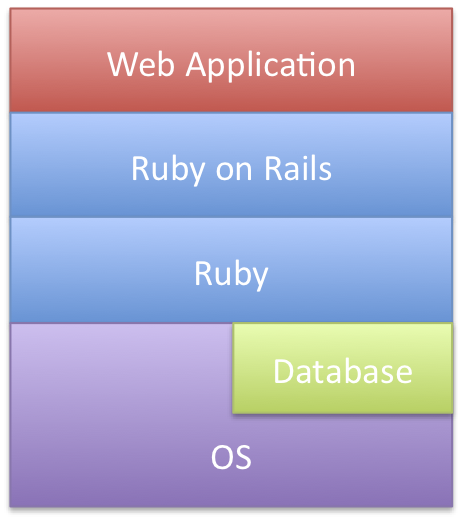
\includegraphics[width=0.5\textwidth]{RailsApplicationStack.png}
\caption{Rails Architektur: Applikation Stack}
\label{fig:Rails Applikation Stack}
\end{figure}
\nocite{Fisher200810}

Ruby On Rails ist nach den Architektur Stilen als Independent Components und Call-and-Return aufgebaut.

Als Independent Components besteht die Architektur aus unabhängigen Komponenten, welche wiederum aus unabhängig ablaufenden Elementen bestehen, die über Nachrichten miteinander interagieren. 

Bei Call-and-Return bzw. dessen Implementierung "'Layered"' werden sämtliche Elemente einzelnen Schichten zugeordnet, die hierarchisch geordnet sind. Jeder dieser Schichten erfüllt eine klar definierte Aufgabe.

Die Basis-Architektur wiederspiegelt sich auch in der Verzeichnisstruktur, welche bei allen Rails Applikationen gleich aufgebaut ist. 

\begin{itemize}
\item \textbf{app:} Hier befindet sich die eigentliche Rails Applikation in der MVC Struktur
\item \textbf{conf:} Applikation Konfigurationsdateien
\item \textbf{db:} Datenbank Schema und Migrations Dateien
\item \textbf{doc:} Dokumentation der Applikation
\item \textbf{lib:} Applicationsspezifischer Code, welcher nicht Teil des MVC Code ist
\item \textbf{log:} Applications Log
\item \textbf{public:} JavaScript, CSS, Bilder und andere statische Inhalte
\item \textbf{script:} Rails Scripts
\item \textbf{test:} Unit-test Code
\item \textbf{tmp:} Cache und Session Informationen
\item \textbf{vender: }Verwendete Fremd-Plugins
\end{itemize}


Neben der einheitlichen Dateistruktur und dem MVC Pattern, haben die Entwickler von Rails das Framework nach dem Design Pattern "'Don't Repeat Yourself"' (DRY) und "'Convention over configuration"' entwickelt.

\begin{figure}[htb]
\centering
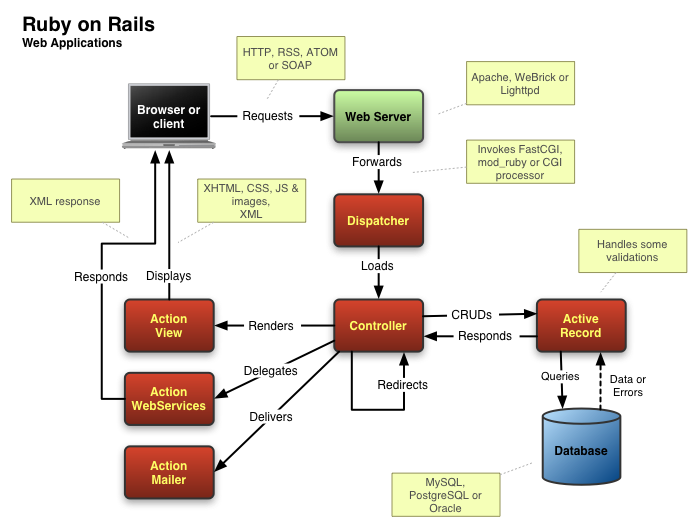
\includegraphics[width=1\textwidth]{rails_architecture.png}
\caption{Architektur: Ruby On Rails [http://blog.roi-office.com]}
\label{fig:RubyOnRails}
\end{figure} 

Die "'Don't Repeat Yourself"' Phylosophie geht davon aus, dass man sich bei der Entwicklung möglich nicht wiederholen soll und stattdessen einen generischen wiederverwendbaren Code entwickeln soll (projektoreintierte Entwicklung). 
Bei Rails wird die Phylosophie auf das ganze Framework angewendet, der Entwickler soll eine Definition nur an einem Ort vornehmen, ohne sich im Quelltext, in der Konfiguration oder in der Dokumentation wiederholen zu müssen. Durch diese vollständige Umsetzung von DRY erspart sich der Entwickler haufenweise Arbeit und verringert gleichzeitig die Fehleranfälligkeit seiner Applikation. Bei einer nachträglichen Anpassung z.B. eines Objekts, Funktion oder Konfiguration muss der Entwickler diese nur an einer Stelle anpassen. Ist der angepasste Quellcode genügend mit Unit-Test abgedeckt, muss der Entwickler bei dieser Anpassung nicht befürchten, dass er neue Fehler in die Applikation eingebaut haben könnte. Natürlich muss man bei diesem stark objektierten Konzeptansatz sich im klaren sein, dass in der Praxis in der Instanz viele Objekte entstehen können, die zwar ähnlich zu einem anderen Objekt sind, aber in dieser Ausprägung nicht weiter vererbt werden kann.

Eine weitverbreitete Eigenschaft von einem viel eingesetzten Applikations-Framework ist es, dass für die Verwendung des Frameworks grosse zum Teil komplexe Konfigurationen vorgenommen werden müssen. Mit der Philosophie "'Convention over configuration"' wollten die Rails Entwickler den Anwendern ihres Frameworks diese Arbeit ersparen. So verhält sich Rails in den meisten Fällen so, wie man es erwarten würde, ohne eine Spezifikation in einer Konfigurationsdatei vornehmen zu müssen.  So weiss z.B. der Routing Mechanismus von Rails ohne eine Konfiguration, welche Klasse und Methode den Seitenaufruf abhandeln muss. Wenn notwendig und gewünscht können diese Standardverhalten einfach überschrieben werden und geben dem Entwickler somit genügend Flexibilität.


\subsection{Datenmodell}

Das Datenmodell soll nach Möglichkeit die reale Welt abbilden, um die gegebenen Anforderungen und die Eigenschaften der Objekte im Datenmodell zu erfüllen. Es wurden folgende Überlegungen gemacht:

\begin{itemize}
\item Ein Cluster besteht aus mindestens zwei oder mehr Servern.
\item Ein Server kann Mitglied eines Clusters sein, oder stand-a-lone betrieben werden.
\item Für die Hochverfügbarkeit eines Clusters ist es wichtig zu wissen, in welcher Site ein Server steht. Aus diesen Grund ist ein Server immer einer Site zugeordnet.\newline
\end{itemize}


\begin{itemize}
\item Ein Server kann ein oder mehrere Volumemanger installiert haben.
\item Ein Server hat ein oder mehrere Disks, wobei es sich um Serverdisks oder LUN Disks handeln kann.
\item Ein Server kann Mitglied eines Clusters sein.
\item Ein Server hat ein oder mehrere Volumemanger
\item Ein Server befindet sich in einem Rechenzentrum/Site.
\item Ein Server hat ein oder mehre Disks.\newline
\end{itemize}


\begin{itemize}
\item Eine Disk kann ein Serverdisk oder LUN-Disk sein.
\item Eine Serverdisk ist immer einem Server zugeteilt. 
\item Eine LUN-Disk kann ein oder mehreren Servern zugeteilt sein.
\item Eine Disk wird nicht in Partitionen aufgeteilt.
\item Eine Disk kann für einen Volume-Manager verwendet werden.
\item Der Volumemanager bestimmt die dazugehörigen Objekte für die Disk.\newline
\end{itemize}


\begin{itemize}
\item Ein Physical Volume gehört immer einer Disk an.
\item Ein Physical Volume kann einer Volume Group zugeordnet werden.\newline
\end{itemize}


\begin{itemize}
\item Eine Volume Group besteht immer aus einer oder mehreren Physical Volumes.
\item Eine Voume Group kann eine oder mehrere Logical Volume Groups haben.\newline
\end{itemize}


\begin{itemize}
\item Ein Logical Volume gehört immer einem Volume Group an.
\item Ein Logical Volume hat eine Filesystem.\newline
\end{itemize}


\begin{itemize}
\item Ein Filesystem gehört immer einem Logical Volume an.
\item Ein Filesystem hat ein Mountpoint.\newline
\end{itemize}

Das im Abbild \ref{fig:Datenmodell} dargestellte Datenmodell, zeigt die Objekte und deren Verbindungen zueinander, zusätzlich enthält es eine mögliche Erweiterung für den Oracle ZFS Volume Manager.

\begin{figure}
\centering
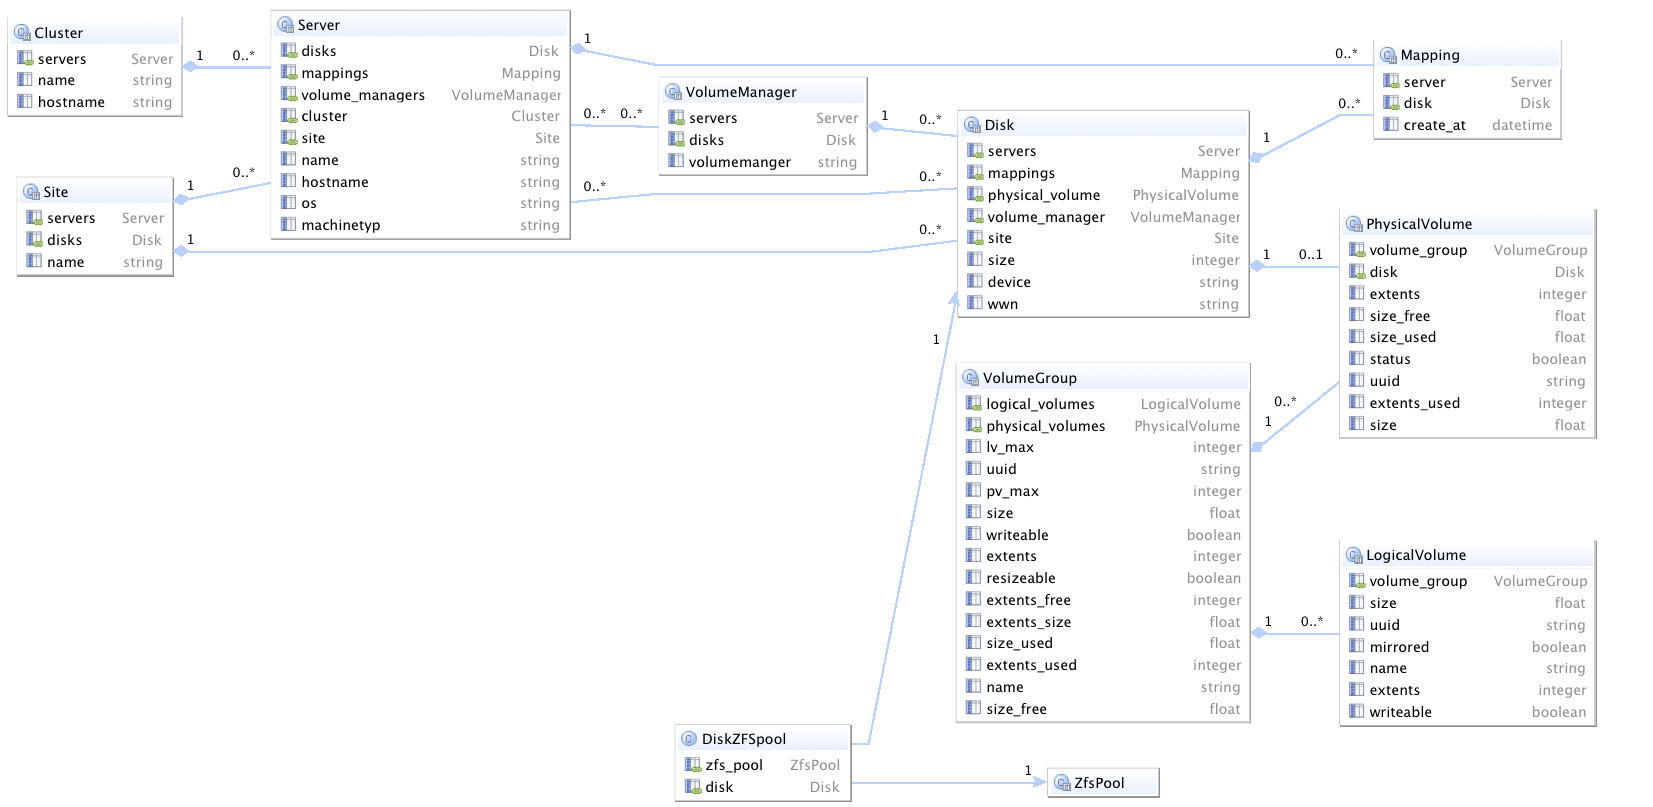
\includegraphics[width=1.5\textwidth, angle= 90]{DatenModell2.png}
\caption{Architektur: Datenmodell}
\label{fig:Datenmodell}
\end{figure}

\newpage
\subsection{LVM-Engine}
Die LVM-Engine inklusive Client-Server Kommunikation wird als Libary-Module für das Web-Framework umgesetzt. Somit ist die Logik der LVM-Engine vom Web-Framework gelöst und kann für andere Projekte wieder verwendet werden. 

\subsubsection{ruby-lvm-wrapper}

Das von den Entwicklern Matthew Kent und John Hampton  auf github veröffentlichte Projekt ruby-lvm-wrapper\footnote{\href{https://github.com/johnhampton/ruby-lvm}{https://github.com/johnhampton/ruby-lvm}} und dessen dazu gehörende Subprojekt ruby-lvm-attributes footnote\footnote{\href{http://rubyforge.org/projects/ruby-lvm-attrib/}{http://rubyforge.org/projects/ruby-lvm-attrib/}}, bietet eine gute Ausgangslage für die LVM-Engine.

Der LVM-\gls{Wrapper} des Projekts liest alle Logical Volumes, Logical Volume Segments , Volume Groups, Physical Volumes und Physical Segments aus einem lokalen Server aus und gibt diese als Ruby Objekt  zurück. Die Attribute der einzelnen LVM Objekten sind pro Objekt im \gls{YAML} Format definiert und in das separate Subprojekt ruby-lvm-attributes ausgelagert. Somit ist die Definition der Objekte vom eigentlichen Quellcode entkoppelt. Für jedes Attribut wird in der \gls{YAML} Datei eine \textit{\/:methode} mit dem LVM Attribute Namen, \textit{\/:type\_hint} mit dem Datentyp des Atttribues, \textit{\/:column} Name des Attributes im RubyObjekt und \textit{\/:description} mit der Beschreibung definiert. Ein Beispiel einer Definition wird in dem Listing \myref{lst:YAML} gezeigt. 
Von der LVM Version abhängig wird im ruby-lvm-attributes Projekt ein Gruppe von YAML Dateien für die Objekte erstellt.

\lstset{language=Ruby, basicstyle=\footnotesize, showstringspaces=false, tabsize=2}
\lstinputlisting[label=lst:YAML,caption=YAML: Beispiel Code aus \Code{PVS}]{DVD/Listings/pvsyaml.txt}

Für die Ausführung und das Auslesen der Ausgabe-Kanäle (englisch: streams), verwendet der Wrapper das \gls{API}  \gls{POpen4}\footnote{\href{https://github.com/pka/popen4}{https://github.com/pka/popen4}} von John-Mason und P. Shackelfords. POpen4 erstellt für die Ausführung der einzelnen Befehlen einen childprocess. POpen4 liest dabei die von POSIX Stream stdin, stdout und stderr aus.
\nocite{TomZrner}

\begin{itemize}
\item \textbf{stdin} ist der Eingabe-Kanal, meistens mit der Tastatur verbunden.
\item \textbf{stdout} ist der Ausgabe-Kanal einer Shell und wird normalerweise auf dem Terminal ausgegeben.
\item \textbf{stderr} ist der Fehler-Ausgabe-Kanal. Die Fehler werden standardmässig auf dem gleichen Gerät wie stdout ausgegeben.
\end{itemize}




\subsubsection{Anpassungen am ruby-lvm-wrapper}

Damit das Projekt ruby-lvm-wrapper die Anforderungen der LVM-Engine erfüllt, muss das Projekt angepasst und erweitert werden. Das Projekt wurde deshalb in einer Forke Version vom ursprünglichen Projekt abgespaltet.

Im ursprünglichen Ruby-lvm-wrapper Projekt, gibt es keinen Wrapper für die LVM Funktionen für das Erstellen und Modifizieren von LVM Objekten. Manipulationen sind zwar indirekt über die RAW Schnittstelle möglich, indem man die LVM Befehle der Schnittstelle übergibt. Dies bedeutet aber, dass die Logik ausserhalb der Ruby-lvm-wrapper zu implementieren ist. Die RAW-Schnittstelle wird deshalb im Forke durch weitere Wrappers für das Erstellen von Physical Volumes, Volume Groups und Logical Volumes ersetzt.

Das Auslesen von LVM Objekten und das Ausführen von Commandline Befehlen ist im ursprünglichen Ruby-lvm-wrapper Projekt auf den lokalen Rechner beschränkt. Die Ausführung im Fork wird mit einer Client-Server Software ersetzt bzw. ergänzt.

Ruby-lvm-wrapper prüft das System bei der Initialisierung auf die LVM Version des Systems und verwendet dazu je Version die YAML Dateien von Projekt ruby-lvm-attrib für das Auslesen der Objekt-Attribute. Weil pro Version die YAML Dateien vorhanden sein müssen,  birgt dies die folgenden Nachteile:
\begin{itemize}
\item Der Verwaltungsaufwand steigt mit der Anzahl der Versionen.
\item Die LVM-Engine könnte nach einer Aktualisierung eines Systems mit Patches, nicht mehr kompatibel (läuffähig) sein, wenn die Version von LVM wechselt.
\end{itemize}

Aus diesen Grund wird im Fork nur die im Datenmodell verwendeten Objekt-Attribute ausgelesen. Zusätzlich wird das Projekt ruby-lvm-attrib in den Fork integriert, was den Vorteil bringt, nicht mehr zwei Projekte parallel pflegen zu müssen.

Die Abbildung \myref{fig:Classdiagramm} zeigt das Klassendigramm nach der Anpassung.

\begin{figure}
\centering
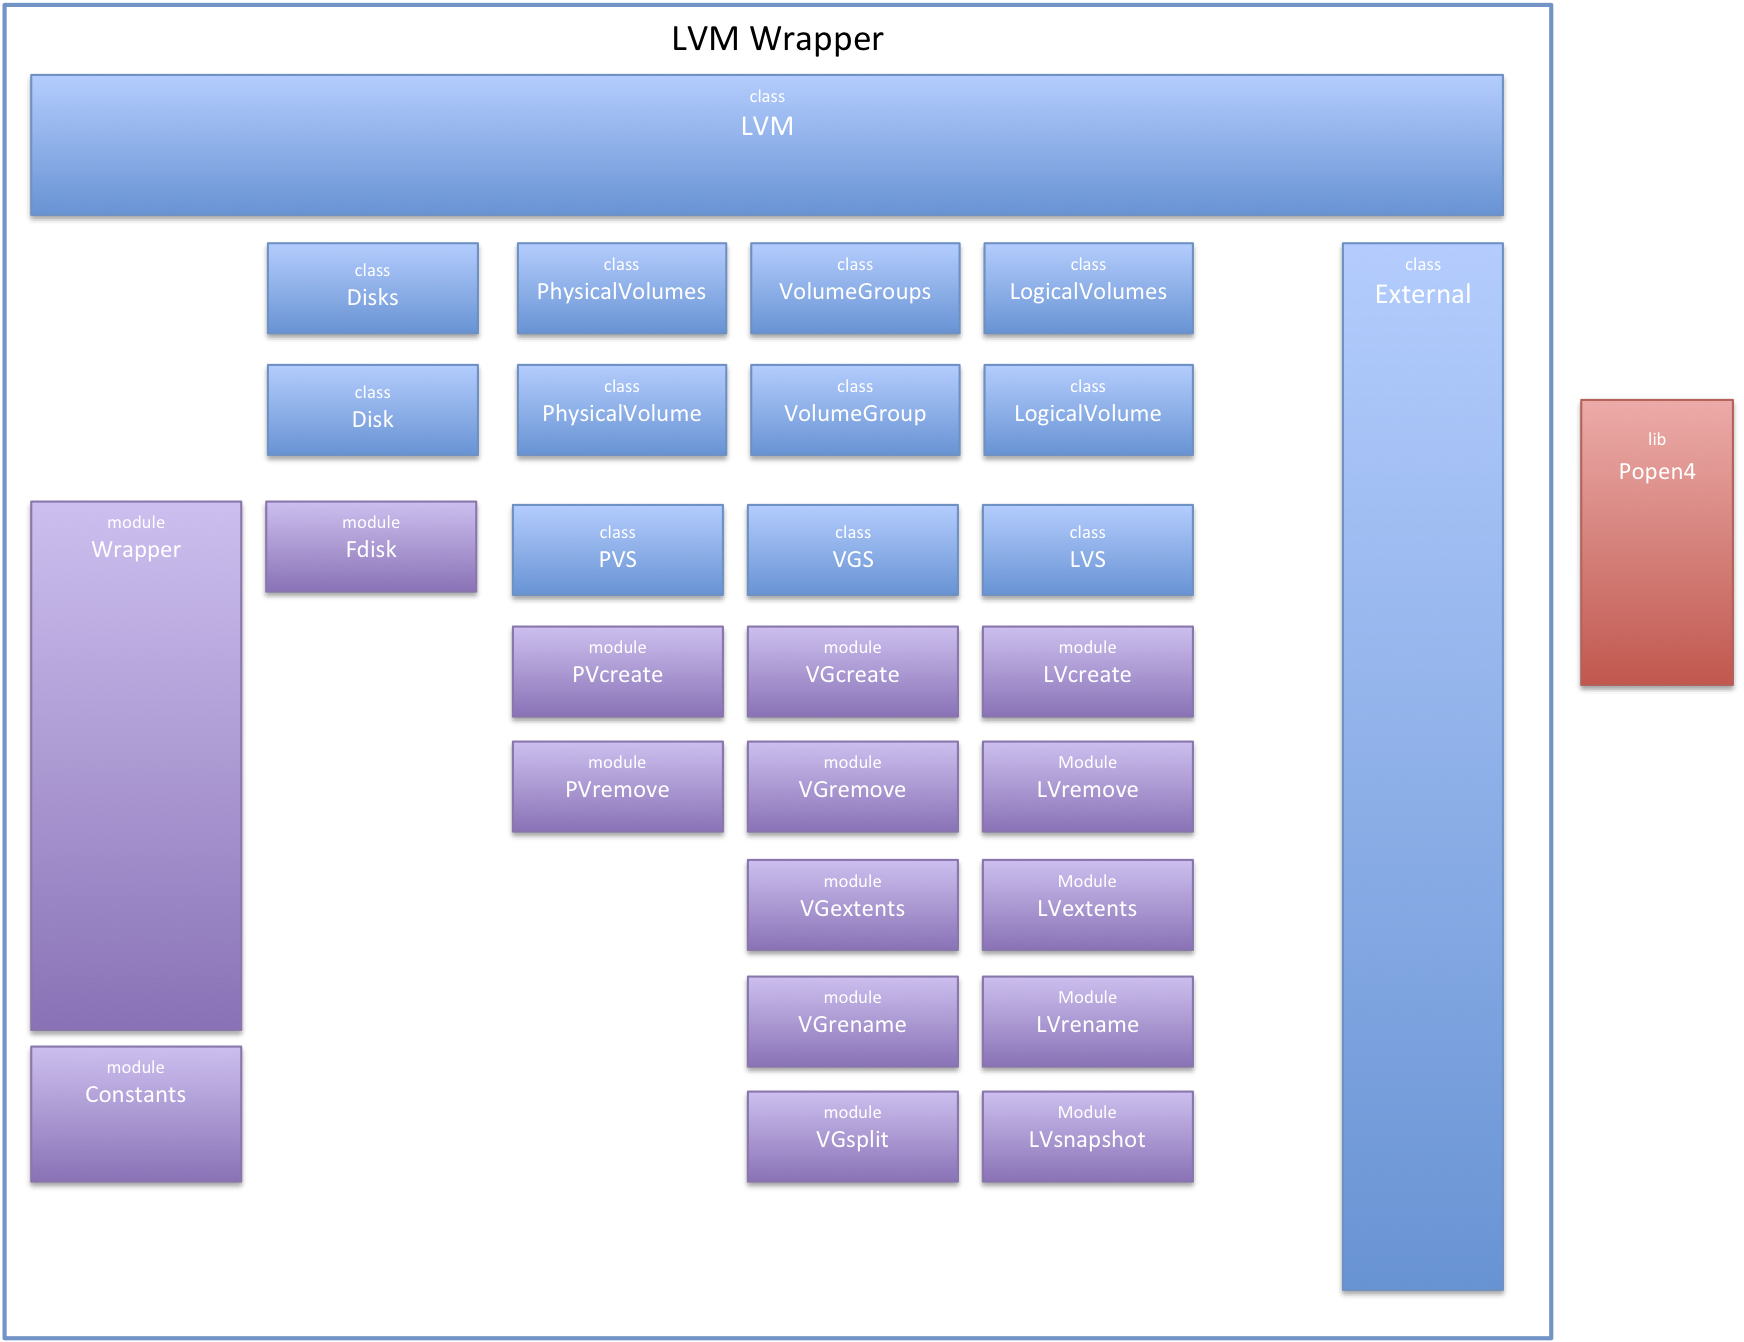
\includegraphics[width=1.5\textwidth , angle= 90]{ClassDiagramLVMWrapper.png}
\caption{Architektur: Klassendiagramm LVM Wrapper}
\label{fig:Classdiagramm}
\end{figure}

\subsection{Objekte Auslesen}
\subsubsection{Lokale Disk auslesen}
 
Die SCSI Disks, welche vom Linux-Kernel Ring erkennt werden, können mit \textit{dmesg} ausgelesen werden.

Befehl:\newline 
\Shell{ dmesg | grep "'SCSI device"' | uniq}
Ausgabe Beispiel:\newline
\Shell{SCSI device sda: 16777216 512-byte hdwr sectors (8590 MB)}

Aus der Ausgabe lässt sich der Gerätename (sda), die Sektorgrösse (512-byte), die Sektoren Anzahl (16777216) auslesen. Mit diesen Angaben lässt sich die Diskgrösse in byte berechnen.

\begin{equation}
Grösse In Byte = Sektorgrösse * Anzahl Sektoren
\end{equation}

\subsubsection{Physical Volumes auslesen}

LVM bietet die Möglichkeit, angepasste Reports der LVM Objekte auszugeben. Somit kann die Ausgabe optimal für das automatische Auslesen per Parser vorbereitet werden.

Befehl:\newline
\Shell{ pvs --separator="';"' --noheadings --nosuffix --units=b --unbuffered}
\Shell{ --options pv\_name,pv\_uuid,pv\_size,pv\_used,pv\_pe\_count,}
\Shell{ pv\_pe\_alloc\_count,pv\_attr,vg\_uuid}

Ausgabe Beispiel:\newline
\Shell{ /dev/sdb;hAL4Ok-vah7-V682-eQqh-n8Wj-geMA-JJKyqV;}
\Shell{ 213909504;0;51;0;a-;MTzZmV-yQua-cycm-msiv-fUM4-5718-wbUp1u}

Das Zeichen zwischen den einzelnen Attributen kann mit der Option --separator bestimmt werden. Bei der Ausgabe wird standardmässig eine Beschriftungzeile ausgegeben. Diese kann mit der Option --noheadings übersteuert werden. Die Einheit der Ausgabe kann mit der Option --units bestimmt werden. Für die Engine wird die Einheitsgrösse Bytes gewählt, somit werden keine kommaseparierten Zahlen ausgegeben.

\subsubsection{Volume Groups auslesen}

Befehl:\newline
\Shell{ vgs --separator=; --noheadings --nosuffix --units=b --unbuffered}
\Shell{ --options vg\_name,vg\_uuid,vg\_size,vg\_free,vg\_extent\_count,}
\Shell{ vg\_extent\_size,pv\_max,lv\_max,lv\_attr,vg\_uuid}

Ausgabe Beispiel:\newline
\Shell{ test;MTzZmV-yQua-cycm-msiv-fUM4-5718-wbUp1u;}
\Shell{ 213909504;213909504;51;4194304;0;0;wz--n-}

\subsubsection{Logical Volumes auslesen}


\Shell{ lvs --separator="';"' --noheadings --nosuffix --units=b --unbuffered}
\Shell{ --options lv\_name,lv\_uuid,lv\_size, pv\_used,pv\_pe\_count,}
\Shell{ pv\_pe\_alloc\_count,pv\_attr, vg\_uuid}



\subsection{Client-Server}
Die Client Server Komponente wird mittels Secure Shell (SSH) realisiert. Diese hat gegenüber einem proprietären Socket - oder einer XMLRPC Lösung den Vorteil, dass auf dem Client keine zusätzliche Software-Installation notwendig ist, die verteilt und später gewartet werden muss. Neue Anpassungen an der Software müssen nur auf einem zentralen Server installiert werden und vereinfacht somit den Versionenwechsel.

SSH gehört zu den Internet Standard Protokoll und ist unter den Request for Comments (\gls{RFC}) 4250\footnote{\href{http://www.ietf.org/rfc/rfc4250.txt}{http://www.ietf.org/rfc/rfc4250.txt}}, 4251\footnote{\href{http://www.ietf.org/rfc/rfc4251.txt}{http://www.ietf.org/rfc/rfc4251.txt}}, 4252\footnote{\href{http://www.ietf.org/rfc/rfc4252.txt}{http://www.ietf.org/rfc/rfc4252.txt}}, 4253\footnote{\href{http://www.ietf.org/rfc/rfc4253.txt}{http://www.ietf.org/rfc/rfc4253.txt}} und 4254\footnote{\href{http://www.ietf.org/rfc/rfc4254.txt}{http://www.ietf.org/rfc/rfc4254.txt}} standardisiert. Der SSH Server ist bei den wichtigen Linux Distributionen im Enterprice Umfeld standardmässig installiert und aktiviert. Mit SSH ist es möglich, auf einem entfernten Rechner bzw. Server, CLI befehle auszuführen, als würde man sich direkt am Terminal des Systems befinden.
Durch die relative einfach und sichere Nutzung, wird SSH von vielen Konfigurations-Applikationen verwendet, um Server zu verwalten.


\subsection{Kommunikation}
Das Anwendungs-Protokoll SSH kommuniziert über TCP auf dem Standard Port 22. Für die Kommunikation zwischen Server und Client sind keine weiteren Ports mehr nötig. Da SSH oft für die Server-Administration verwendet wird, ist dieser Port auf vielen Firewall geöffnet. Somit sind meist keine langwierigen Firewall Change-Requests notwendig.


\subsection{Sicherheit}
Mit dem Einsatz von SSH als Client-Server Komponente, ist durch die symmetrische Verschlüsselung mittels \gls{TrippleDES}, \gls{BlowFisch} oder \gls{AES} die Kommunikation sichergestellt. Damit sind keine Manipulationen beim Übertragen der Befehle auf den Client möglich. 

Für die Authentifizierung und den Schlüsselaustausch kann bzw. wird bei SSH das Public-Key Verfahren mittels \gls{RSA} eingesetzt. Mit diesem Verfahren ist sichergestellt, dass sich gleichzeitig nur ein Benutzer bzw. eine Applikation am System anmelden kann, wenn dieser im Besitz des privaten Schlüssels ist.


Für die Ausführung von LVM Befehlen auf dem System sind hohe Berechtigungsrechte auf dem System notwendig. Würde ein Angreifer Zugriff auf den Server erhalten, könnte er auf allen Clients Befehle mit hohen Rechten ausführen. Durch den Einsatz von \gls{SUDO} kann auf dem Client ein Benutzer mit niedrigen Rechten angelegt werden, welcher mit \gls{SUDO} nur die LVM-Befehle mit hohen Rechten ausführen kann.


\section{Testing}
Ein ausgereiftes white-box Testing hat einen spürbaren Einfluss auf die Code-Qualität. Ferner bietet es dem Entwickler die Möglichkeit, schneller auf Anforderungsänderungen einzugehen. Der Entwickler hat bei einem Projekt, bei welchem der Code gut mit Units-Test abgedeckt ist, bei Anpassungen am bestehenden Code eine gute Leitlinie, welche ihm hilft, weitgehend fehlerfrei zu entwickeln.
Für die Entwicklung des Projektes wird das in Ruby implementierte UnitTest Framework verwendet.


\chapter{Prototyp LVM Engine}
\label{cha:Prototyp}



\section{Ausgangslage}
Mit dem Prototyp soll die Machbarkeit der Entwicklung einer LVM Engine aufgezeigt werden.
Die LVM Engine ist der Teil der Anwendung, welche auf dem Clients die LVM-Befehle ausführt, um LVM Objekte einzulesen und anzulegen. Die LVM Engine baut auf dem Projekt ruby-lvm-wrapper auf. Dadurch sind die Funktionen für das Einlesen der LVM Objekte bereits umgesetzt.

\section{SSH Client}
Im ruby-lvm-wrapper wurden die LVM an die Funktion cmd des Module External übergeben. Für das Ausführen eines Befehles auf einem entfernten Rechner habe ich die Funktion cmd mit der Funktion Parameter Server ergänzt. Ursprünglich wollte ich für SSH die Ruby Libary NET::SSH verwenden. Für die Sicherheit auf dem Client sollten die LVM Befehle mittels SUDO auf dem System ausgeführt werden. Für das Ausführen von SUDO ist eine Shell notwendig. Die Libary hat diese jedoch nicht unterstützt, weshalb ich die LVM Befehle an den SSH Client des Systemes als Parameter übergeben habe. 

Mit der Option \textbf{-q}  (Quite Mode) wird verhindert, dass Login Banner Informationen des Clients nicht ausgegeben werden. Die Unterdrückung der Ausgabe hat den Vorteil, dass keine störende Zeichen oder Zeilen für das Parsen ausgegeben werden. Für SUDO wird mit der Option \textbf{-t} in doppelter Ausführung eine TTY alloziert. Der Loginname wird mit der Option \textbf{-l} (Login) und dem Benutzernamen definiert. Mit der Option \textbf{-i} und dem Pfad zum SSH Private-Key des Benutzers kann die PublicPrivate Key Authentifizierung von SSH verwendet werden.

Der Auszug der Klasse External, welche im Listing \myref{lst:KlassExternal} abgebildet ist, zeigt den ganzen SSH Befehl.

Für alle zu verwendeten Clients wird der gleiche SSH-Key und der gleiche SSH-Benutzer verwendet. Somit kann dieser vom System klar als Application-Benutzer identifiziert werden und allenfalls automatisch über ein Konfiguration Management Tool angelegt werden. Einfachheitshalber kann man den SSH Benutzer und den Pfad zu dessen Private Key über eine AppConfig File im YAML Format für die Engine konfigurieren bzw. bereitstellen.

\lstset{language=Ruby, basicstyle=\footnotesize, showstringspaces=false, tabsize=2}
\lstinputlisting[label=lst:KlassExternal,caption=LVM-Engine: Klass \Code{External}]{DVD/ruby/external.rb}

Zusätzlich zu den SSH Anpassungen wurden in der Klasse der Code für die pOpen4 Stream-Verarbeitung vereinfacht. 

\section{Physical Volume erstellen}
Für das Erstellen von Physical Volumes habe ich einen Wrapper für den LVM-Befehl pvcreate als Module PVcreate gebaut. Das Module PVcreate stellt die Funktion pv\_create zur Verfügung. Die Funktion pv\_create verlangt eine Device Objekt als Parameter. Für das Device-Objekt wird geprüft, ob dessen Attribute "Partition" und "Physical Volume Label" gesetzt sind. Ist dies nicht der Fall, wird anhand des Device Namen ein Physical Volume angelegt.

\lstset{language=Ruby, basicstyle=\footnotesize, showstringspaces=false, tabsize=2}
\lstinputlisting[label=lst:ModulePVCreate,caption=LVM-Engine: Module \Code{PVCreate}]{DVD/ruby/pvcreate.rb}

\section{VolumeGroup erstellen}
Das Module VGCreate bietet die beiden Funktionen vg\_create und vg\_create\_cluster an. Beide Funktionen erstellen anhand eines oder mehrerer Physical Volume Objekte eine Volume Group mit dem Unterschied, dass bei der Funktion  vg\_create\_cluster ein Clustered Volume Group erstellt wird. Das Physical Volume Object wird in einem Array zusammen mit dem gewünschten Volume Group Namen an die Funktionen übergeben. Die Funktionen prüfen alle übergebenen Physical Volume Objekte, ob diese bereits einer Volume Group zu geordnet sind. Ist diese nicht der Fall, wird die Volume Group mit dem gewünschten Namen erstellt. 

\lstset{language=Ruby, basicstyle=\footnotesize, showstringspaces=false, tabsize=2}
\lstinputlisting[label=lst:ModuleVGCreate,caption=LVM-Engine: Module \Code{VGCreate}]{DVD/ruby/vgcreate.rb}

\section{Logical Volume erstellen}
Für das Erstellen eines Logical Volumes wurde ein Wrapper-Modul für den LVM-Befehl LVcreate erstellt. Das Module LVcreate bietet die Möglichkeit, gespiegelte und nicht-gespiegelte Logical Volumes auf einer Volume Group anzulegen. Dabei kann die Grösse jeweils in Extents oder in Bytes definiert werden.
Den dafür benötigten vier Funktionen werden der Logical Volume Name, das Volume Group Objekt und die Grösse übergeben. Die Funktion prüft, ob für das Volume Objekt genügend Speicherplatz vorhanden ist, ein Logical Volume mit der gewünschten Grösse anzulegen.

\lstset{language=Ruby, basicstyle=\footnotesize, showstringspaces=false, tabsize=2}
\lstinputlisting[label=lst:ModuleLVCreate,caption=LVM-Engine: Module \Code{LVCreate}]{DVD/ruby/lvcreate.rb}

\section{Logical Volume entfernen}
Für das Entfernen eines Logical Volume wurde das Module LVRemove entwickelt. Das Module bietet die Funktion lv\_remove an.

\lstset{language=Ruby, basicstyle=\footnotesize, showstringspaces=false, tabsize=2}
\lstinputlisting[label=lst:ModuleLVRemove,caption=LVM-Engine: Module \Code{LVRemove}]{DVD/ruby/lvremove.rb}

\section{Volume Group entfernen}
Das Wrapper Module VGRemove entfernt eine Volume Group, wenn diese keine Logical Volume Objekte enthält.

\lstset{language=Ruby, basicstyle=\footnotesize, showstringspaces=false, tabsize=2}
\lstinputlisting[label=lst:ModuleVGRemove,caption=LVM-Engine: Module \Code{VGRemove}]{DVD/ruby/vgremove.rb}

\section{Physical Volume entfernen}
Das Wrapper Module PVRemove entfernt den Phyiscal Volume Label eines Physical Volume Objektes, wenn dieses keinem Volume Group zugeordnet ist. Die Zuordnung wird anhand des Attributes vg\_uuid geprüft.

\lstset{language=Ruby, basicstyle=\footnotesize, showstringspaces=false, tabsize=2}
\lstinputlisting[label=lst:ModulePVRemove,caption=LVM-Engine: Module \Code{PVRemove}]{DVD/ruby/pvremove.rb}

\section{Volume Group erweitern}
Das Wrapper Module VGExtents erweitert ein Volume Group Object, nach denselben Kriterien wie beim Erstellen einer Volume Group.

\lstset{language=Ruby, basicstyle=\footnotesize, showstringspaces=false, tabsize=2}
\lstinputlisting[label=lst:ModuleVGExtend,caption=LVM-Engine: Module \Code{VGExtend}]{DVD/ruby/vgextend.rb}


\section{Logical Volume erweitern}
Das Wrapper Module LVExtents erweitert ein Logical Volume Object, nach denselben Kriterien wie beim Erstellen eines Logical Volumes.

\lstset{language=Ruby, basicstyle=\footnotesize, showstringspaces=false, tabsize=2}
\lstinputlisting[label=lst:ModuleLVExtend,caption=LVM-Engine: Module \Code{LVExtend}]{DVD/ruby/lvextend.rb}

\section{Quellcode}
Das Projekt befindet sich auf der Social Coding Plattform "Github" 
\url{https://github.com/lutsho/ruby-lvm-ssh}



%\include{Inhalt/MartAnalyse}
%\include{Inhalt/ZitateReferenzen}
%\include{Inhalt/BilderListings}
%\include{Inhalt/AufzaehlungenTabellen}
%\newglossaryentry{Kostenstruktur}{ name={Kostenstruktur}, description={Definition gemäss \url{http://www.wirtschaftslexikon24.net/d/kostenstruktur/kostenstruktur.htm}
Art der Zusammensetzung der Kosten eines Kostenbereichs oder einer Unternehmung während einer Periode aus bestimmten, sich durch Entscheidungen ergebenden Teilen, wie Einzel- und Gemeinkosten, fixe und variable Kosten, Zahl der Kostenarten usw. Die jeweils entstehende Relation zwischen den Kostenteilen hängt von den Kostenbestimmungsfaktoren ab }}

\newglossaryentry{LUN}{ name={LUN}, description={Logical Unit Number kurz LUN, ist eine Nummer um ein Locical Unit bzw. eine SCSI Gerät zu identifizieren. Oft wird bei der Verwendung des Begriffs das Gerät selber gemeint, was technisch nicht ganz korrekt ist. Im Storage Umfeld wird LUN mit Disk gleichgesetzt}}

\newglossaryentry{SAN}{ name={SAN}, description={Storage Area Netzwork, ist ein Netzwerk zur Anbindung von Speicher und Tape, welches von einem Storage-System bzw. Tape-Library eines Servers stammt. Die Server und Storage-Systeme kommunizieren im SAN mit Fibre-Channels }}

\newglossaryentry{Snapshot}{ name={Snapshot}, description={Snapshot ist ein besonderer Speicherbereich, der sämtliche Änderungen zu einem älteren festgelegten Datenbestand aufnimmt. \url{http://en.wikipedia.org/wiki/Snapshot_(computer_storage) }}}

\newglossaryentry{Cluster}{ name={Cluster}, description={Ein Cluster ist ein Verbund von vernetzten Servern, auch Nodes genannt, welche dem Client in Form eines einzelnen Server gesehen wird. Cluster werden meist dazu verwendet, um einen Server-Service hoch verfügbar zu halten, indem ein Cluster Node die Aufgaben eines anderen Cluster Node übernimmt. Zudem werden Cluster für die Erhöhung von Rechenkapazität eingesetzt, wie sie z.B. in der Forschung, Industrie bzw. Metrologie zur Berechnung rechenintensiver Aufgaben verwendet werden. \url{http://de.wikipedia.org/wiki/Computercluster}}}

\newglossaryentry{ClusterNode}{ name={Cluster Node}, description={Ein Cluster Node, oder oft auch nur als Node (zu deutsch Knoten) bezeichnet, ist ein einzelner Server in einem Cluster-Verbund }}

\newglossaryentry{YAML}{ name={YAML}, description={YAML ist eine vereinfachte Auszeichnungssprache zur Datenserialisierung, angelehnt an XML und an die Datenstrukturen in den Sprachen Perl, Python und C. \url{http://de.wikipedia.org/wiki/YAML}}}

\newglossaryentry{POpen4}{ name={POpen4}, description={POpen4 stellt den Ruby Entwicklern eine plattformübergreifende API zur Ausführung von Befehlen in einen Kindprozess, welche die stdout, stderr, stdin stream als auch die Prozess-ID und Exit Status behandelt, zur Verfügung stellt. \url{http://popen4.rubyforge.org/ }}}

\newglossaryentry{Wrapper}{ name={Wrapper}, description={Als Wrapper bezeichnet man in der Informationstechnik ein Stück Software, welches ein anderes Stück Software umgibt (umwickelt). \url{http://de.wikipedia.org/wiki/Wrapper_(Software)}}}

\newglossaryentry{RFC}{ name={RFC}, description={Request for Comments (RFC) sind Dokumente, über Internet, inklusive der technischen Spezifikation und Richtlinien, welche von der Organisation Internet Engineering Task Force entwickelt wurde. "'Das RFC wird erst nach erfolgter Diskussion unter der Aussicht des Internet Architecture Board (IAB) herausgegeben und fungiert als Quasistandard. Jedes RFC enthält eine eindeutige, vorlaufende Nummer, die kein zweites Mal zu gewiesen wird."' \cite{MicrosoftComputerLex}  \url{http://www.rfc-editor.org/}}}

\newglossaryentry{AES}{ name={AES}, description={Advanced Encryption Standard (AES) wurde von US National Institute of Standards and Technology für den Schutz von elektronischen Daten spezifiziert. AES Algorithmus ist eine symetrische Block Chiffrierung, welche mit 128, 192 und 256 bit Schlüssel Daten in Blocks von 128 bit verschlüsseln und entschlüsseln kann. \url{http://www.nist.gov/manuscript-publication-search.cfm?pub_id=901427}}}

\newglossaryentry{RSA}{ name={RSA}, description={RSA ist eine Chiffrierungs Algorithmus für asymetrische Verschlüsselung und wurde von den Mathematikern Ronald L. Rivest, Adi Shamir und Leonard Adleman entwickelt. RSA wird in vielen Verfahren verwendet, in welchen eine sichere Authentifizierung sichergestellt werden muss, unter anderem in SSL, PKI usw. \url{http://www.rsa.com/rsalabs/node.asp?id=2125 }}}

\newglossaryentry{BlowFisch}{ name={BlowFish}, description={BlowFish wurde von Brice Schneider 1993 entwickelt. Der Blowfish Algorithmus ist eine symetrische Block Chiffrierung, welche eine variable Schlüssellänge von 32 bits bis 448 bits Daten verschlüsseln und entschlüsseln kann. \url{http://www.schneier.com/blowfish.html} }}


\newglossaryentry{TrippleDES}{ name={TrippleDES}, description={TrippleDES ist eine Erweiterung des Data Encryption Standards (DES) für die symmetrische Verschlüsselung und Entschlüsselung. TrippleDES verschlüsselt die Daten drei mal mit DES, dabei werden jeweils drei von einander unabhängige Schlüssel verwendet. }}

\newglossaryentry{SUDO}{ name={SUDO}, description={Sudo kommt von dem Befehl su und dem Wort do und erlaubt es System Administratoren-Berechtigung an Benutzer oder Gruppen zu geben und einzelne Befehle als root Benutzer auszuführen. \url{http://www.courtesan.com/sudo/} }}

\newglossaryentry{API}{ name={API}, description={Application Programming Interface (API) auch Anwendungsprogrammierschnittstelle genannt. "'Ein Satz an Routinen, die vom Betriebsystem des Computers für die Verwendung aus Anwendungsprogrammen heraus angeboten werden und diverse Dienste zur Verfügung stellen."' \cite{MicrosoftComputerLex} }}
\chapter{Fazit / Zusammenfassung}
\label{cha:Fazit}

Mit dem Thema Volume Manager Engine habe ich bewusst ein Thema gewählt, welches mir erlaubt, viel neues Wissen anzueignen und mich in neue Technologien einzuarbeiten. Neben den Volume Managern LVM und ZFS war mir die Programmiersprache Ruby zu Beginn der Arbeit nicht bekannt.

Für die Einarbeitung in LVM habe ich mich zuerst mittels Literatur in das Thema eingelesen. Dazu habe ich das Handbuch von RedHat verwendet. Für eine wissenschaftliche Arbeit möchte man sicher noch tiefer in eine neue Technologie hineinblicken, als dies das Studium eines Benutzerhandbuches für Anwender zulässt. Leider war es mir trotz intensiven Recherchen nicht möglich gewesen, an bessere und zuverlässigere Quellen heranzukommen. Beispielsweise ging aus dem Handbuch nicht klar hervor, wie die Segmentierung der Volumes und das Striping der Volumens zusammenhängen. Leider blieb eine anonyme Anfrage in der offiziellen LVM-Mailingliste unbeantwortet und erfolglos.
Andere Fragen versuchte ich anhand von virtuellen Linux Servern, welche ich als Cluster und nicht Cluster-Betrieb ausführte, mir zu erarbeiten. Obwohl diese Vorgehensweise eher aufwendig ist, sammelte ich damit viel Erfahrung und es half mir sehr gut, mich in LVM einzuarbeiten.
 
Anhand von Grafiken und den dazugehörenden Beschreibungen, versuchte ich die Eigenschaften von LVM dem Leser zu erklären. Die Grafiken sollten es dem Leser vereinfachen, die verschiedenen Volume Architekturen, welche LVM unterstützt und wie die einzelnen LVM-Objekte zu einander in Verbindung stehen, zu verstehen. Die Zusammenfassung der wichtigsten Befehle beschreibt, wie sich die aufgeführten Architekturen konfigurieren lassen.
 
Die Anforderungsanalyse für die Applikation habe ich um eine Marktanalyse ergänzt, obwohl diese nicht Ziel der Arbeit war, aber weitere sinnvolle Informationen liefert. Eine Marktanalyse sollte nach meinem Verständnis in keiner Arbeit fehlen, in der es um die Implementation eines neuen Produktes geht. Ohne zu erforschen, welche Produkte und Optionen der Markt für die bestehenden und zukünftigen Technologien bietet und welche davon sich wahrscheinlich durchsetzen werden, sollte man kein Softwareprojekt beginnen. Gerne hätte ich anhand von Gartner-Analysen dargestellt, wie sich der Markt von x86 zu RISC Architekturen voraussichtlich künftig entwickeln wird, jedoch waren diese Analysen nur käuflich zu erwerben und nicht öffentlich zugänglich. Eine Firma hätte sicherlich sich die notwendigen Informationen aus dem Projektbudget geleistet. 
  
Mit dem Prototyp konnte ich aufzeigen, dass eine Umsetzung des von mir erstellten Konzept möglich ist. Für den Prototyp habe ich ein bestehendes Projekt verwendet und mit meinen Anforderungen erweitert. Als Novize in einer neuen Programmiersprache hat es mir geholfen, dass ich mich an bestehenden Codebeispielen orientiert habe und meiner Einschätzung nach eine akurate Architektur erstellt habe.

Für mich persönlich fällt die Zwischenbilanz für diese Arbeit positiv aus. Die Arbeit half mir neues und für meinen Beruf notwendiges Wissen anzueignen, welches ich künftig in meinen Arbeiten einsetzen werde. Auf Wunsch meines Arbeitgebers werde ich mich nach Beendung der Semesterarbeit bei der Entwicklung neuer Storage Managment Tools in der Firma einbringen.
Dieser neue Aufgabenbereich bietet mir neben der Weiterbildung im System-Engineering, einen nahtlosen und idealen Einstieg in die Softwareentwicklung.







% Abkürzungsverzeichnis --------------------------------------------------------

\printglossary[style=altlist,title=Glossar]


% für korrekte überschrift in der Kopfzeile
%\clearpage\markboth{\nomname}{\nomname} 
%\printnomenclature
\label{sec:Glossar}



% Literaturverzeichnis ---------------------------------------------------------
%   Das Literaturverzeichnis wird aus der BibTeX-Datenbank "Bibliographie.bib"
%   erstellt.
% ------------------------------------------------------------------------------
\bibliography{Bibliographie} % Aufruf: bibtex Masterarbeit
\bibliographystyle{natdin} % DIN-Stil des Literaturverzeichnisses

\addchap{Eidesstattliche Erklärung}
Ich, \autor, Matrikel-Nr.\ \matrikelnr, versichere hiermit, dass ich meine Seminararbeit mit dem Thema
\begin{quote}
\textit{\titel} \textit{\untertitel}
\end{quote}
selbständig verfasst und keine anderen als die angegebenen Hilfsmittel benutzt habe. Alle Stellen, die dem Wortlaut oder dem Sinne nach anderen Texten entnommen sind, wurden unter Angabe der Quellen (einschliesslich des World Wide Web und anderer elektronischer Text- und Datensammlungen) und nach den üblichen Regeln des wissenschaftlichen Zitierens nachgewiesen. Dies gilt auch für Zeichnungen, bildliche Darstellungen, Skizzen, Tabellen und dergleichen. Mir ist bewusst, dass wahrheitswidrige Angaben als Täuschungsversuch behandelt werden und dass bei einem Täuschungsverdacht sämtliche Verfahren der Plagiatserkennung angewandt werden können.\\[6ex]


Zürich, den \today


\rule[-0.2cm]{5cm}{0.5pt}

\textsc{\autor} 
 % Selbst�ndigkeitserkl�rung

% Anhang -----------------------------------------------------------------------
%   Die Inhalte des Anhangs werden analog zu den Kapiteln inkludiert.
%   Dies geschieht in der Datei "Anhang.tex".
% ------------------------------------------------------------------------------
\begin{appendix}
    \clearpage
    \pagenumbering{roman}
    \chapter{Anhang}
    \label{sec:Anhang}
    
\section{Projektplanung}

\subsection{Meilensteine}

\begin{figure}[H]
\centering
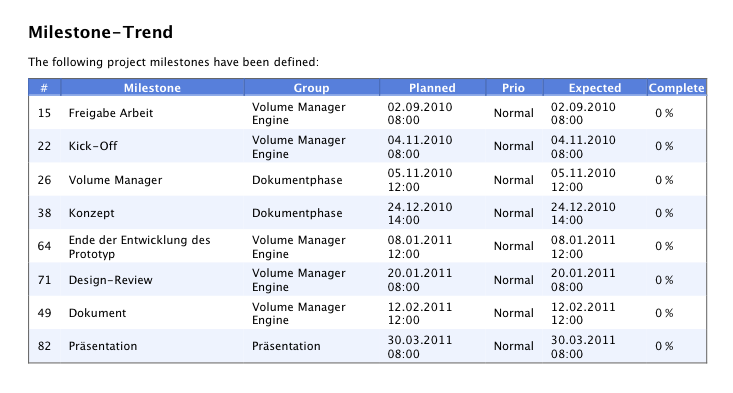
\includegraphics[width=1.2\textwidth]{Milestones.png}
\caption{Projektplanung: Meilensteine}
\label{fig:Meilensteine}
\end{figure}

\subsubsection{Trend}

\begin{figure}[H]
\centering
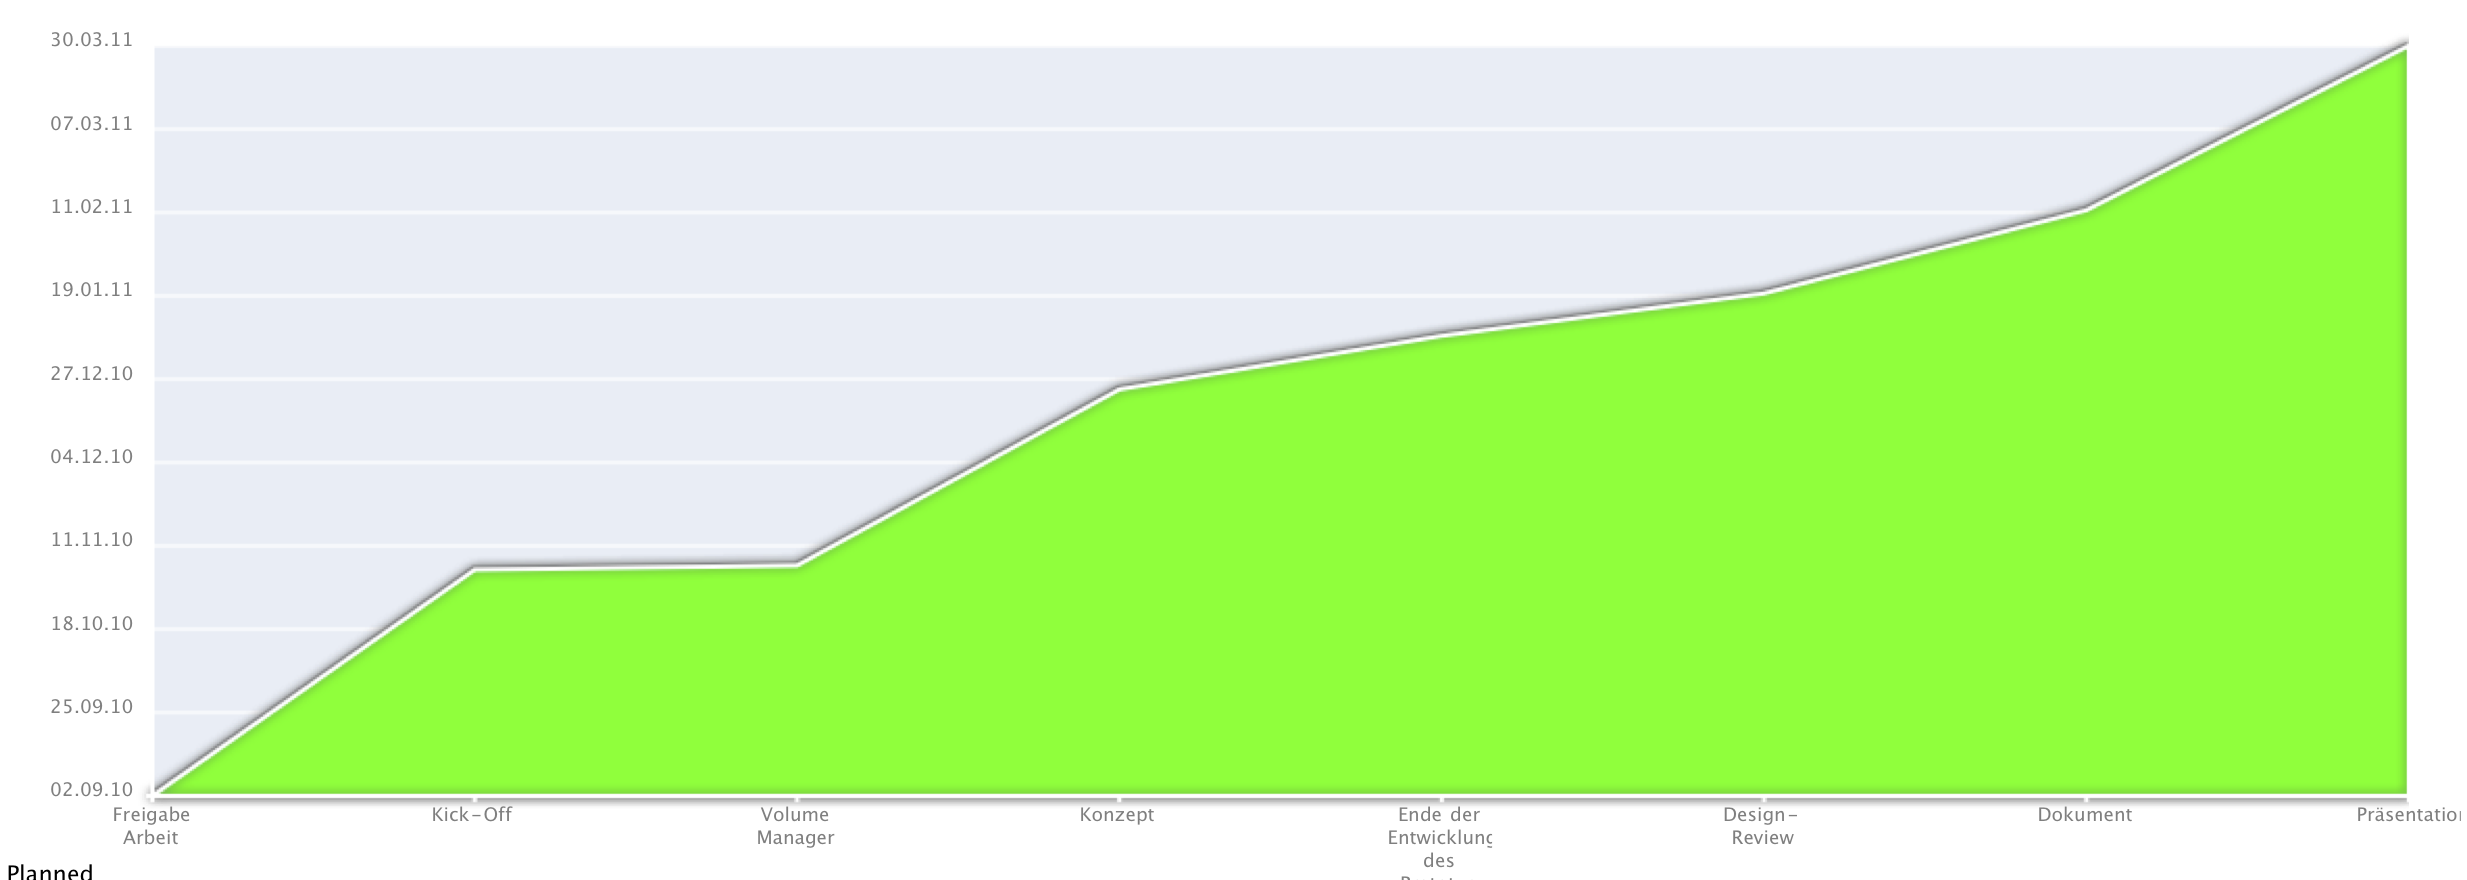
\includegraphics[width=1.4\textwidth, angle= 90]{MilestonesTrend.png}
\caption{Projektplanung: Meilensteine Trend}
\label{fig:MeilensteinTrend}
\end{figure}

\subsection{Netzplan}

\begin{figure}[H]
\centering
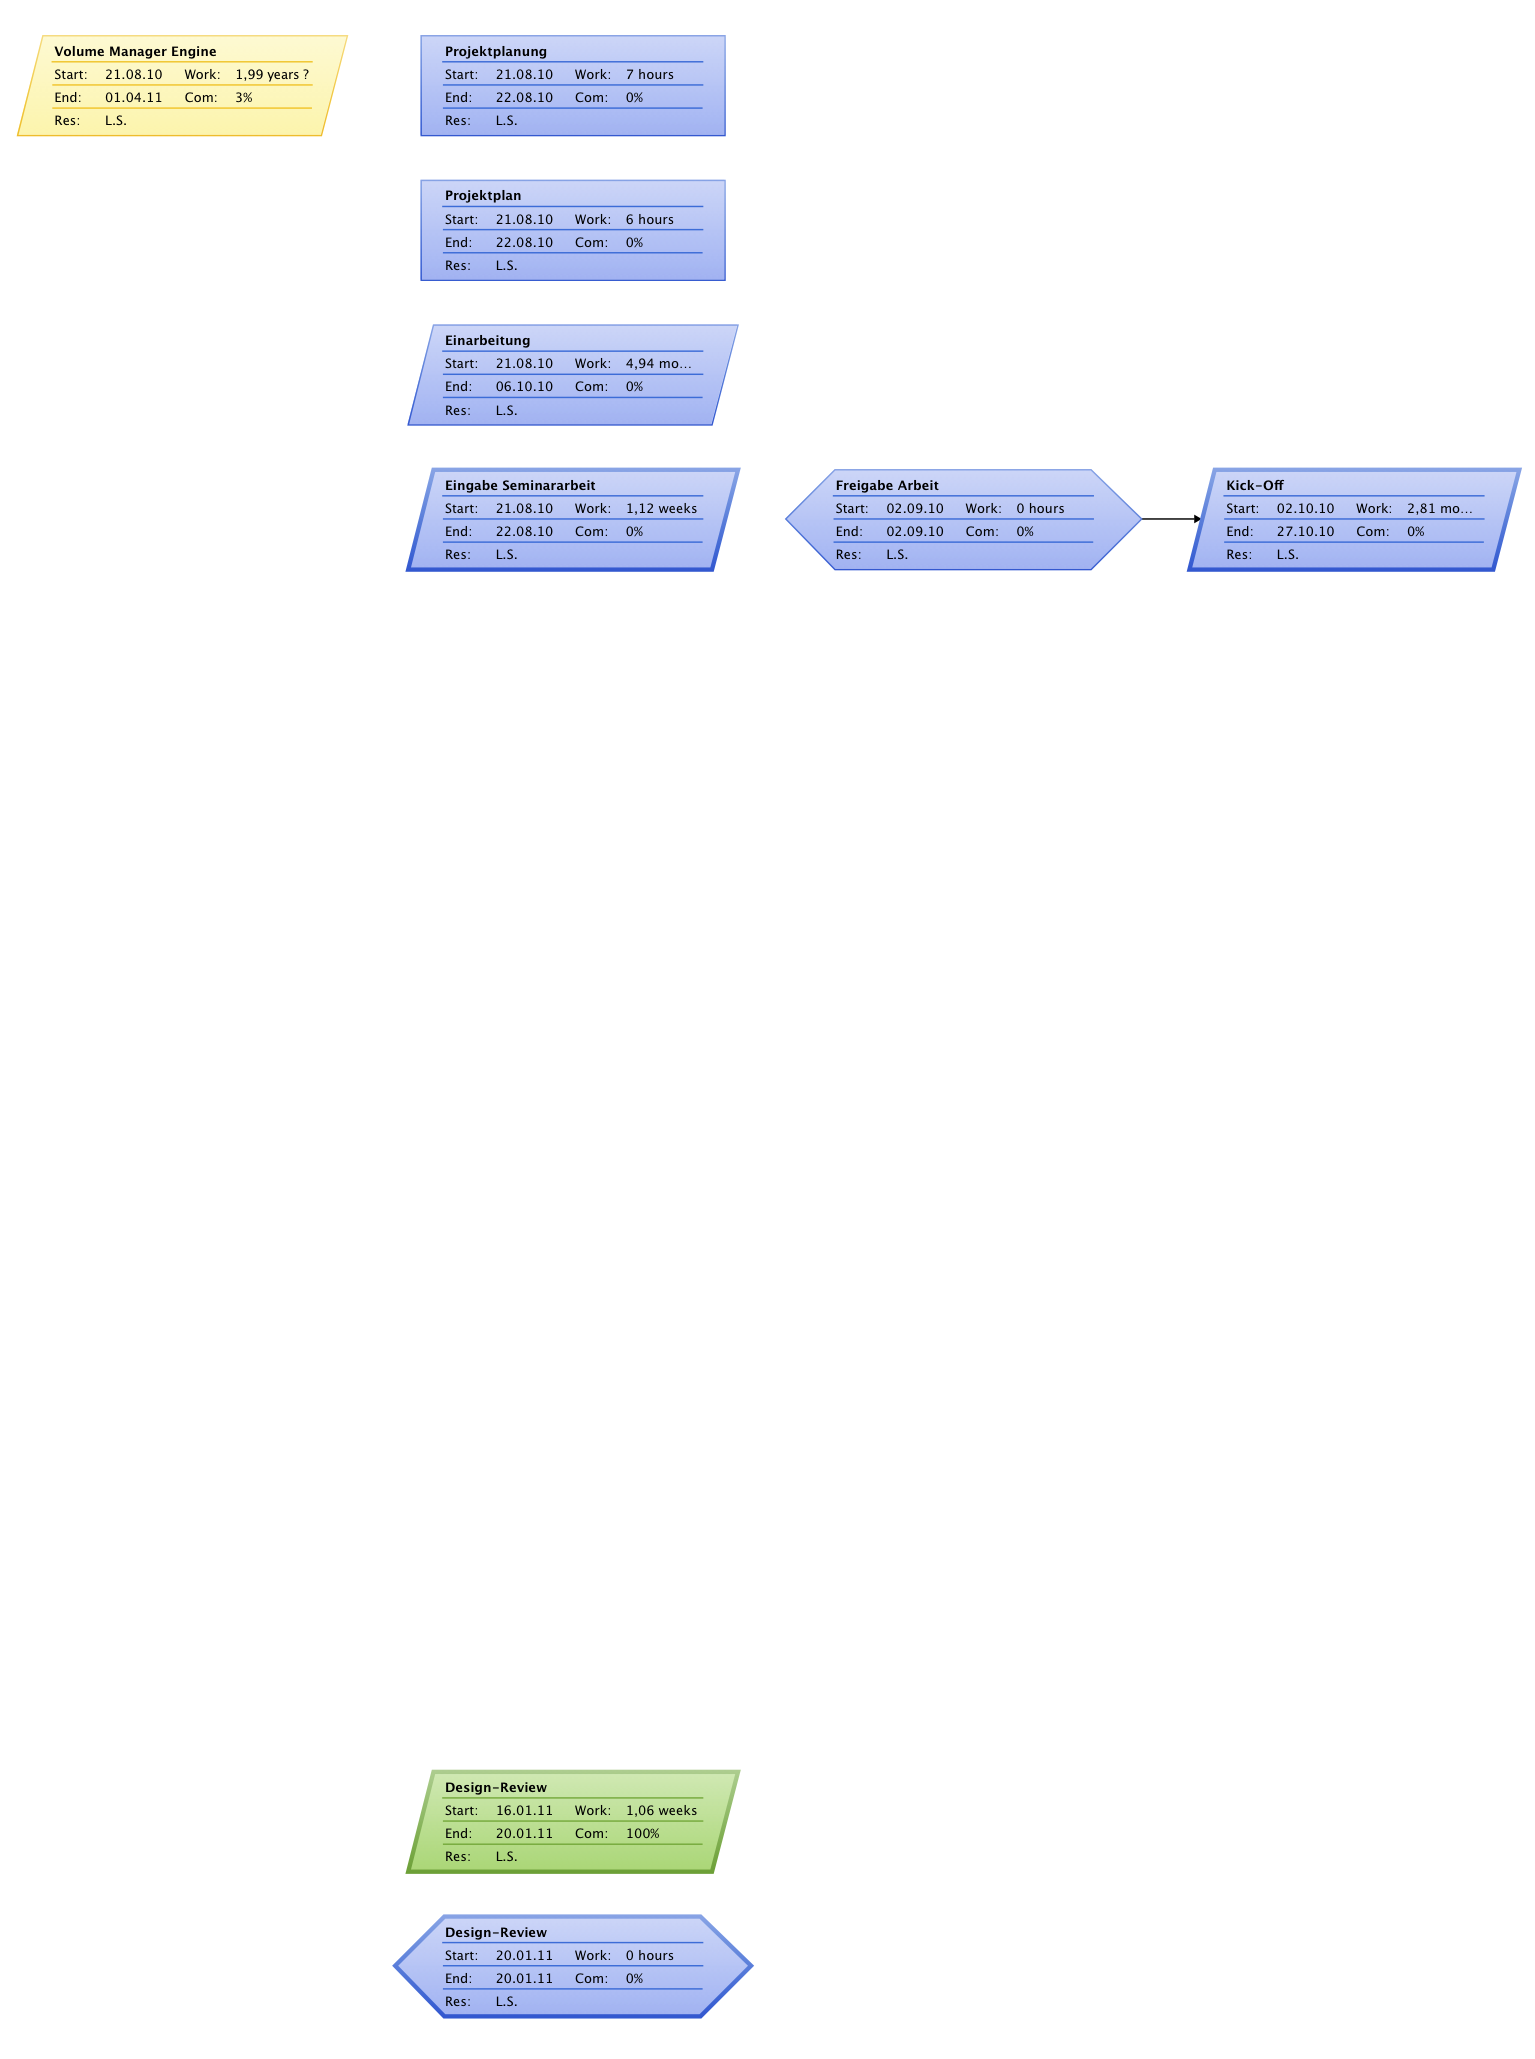
\includegraphics[width=1\textwidth]{Netzplan1.png}
\caption{Projektplanung: Netzplan Teil 1}
\label{fig:Netzplan1}
\end{figure}

\begin{figure}[H]
\centering
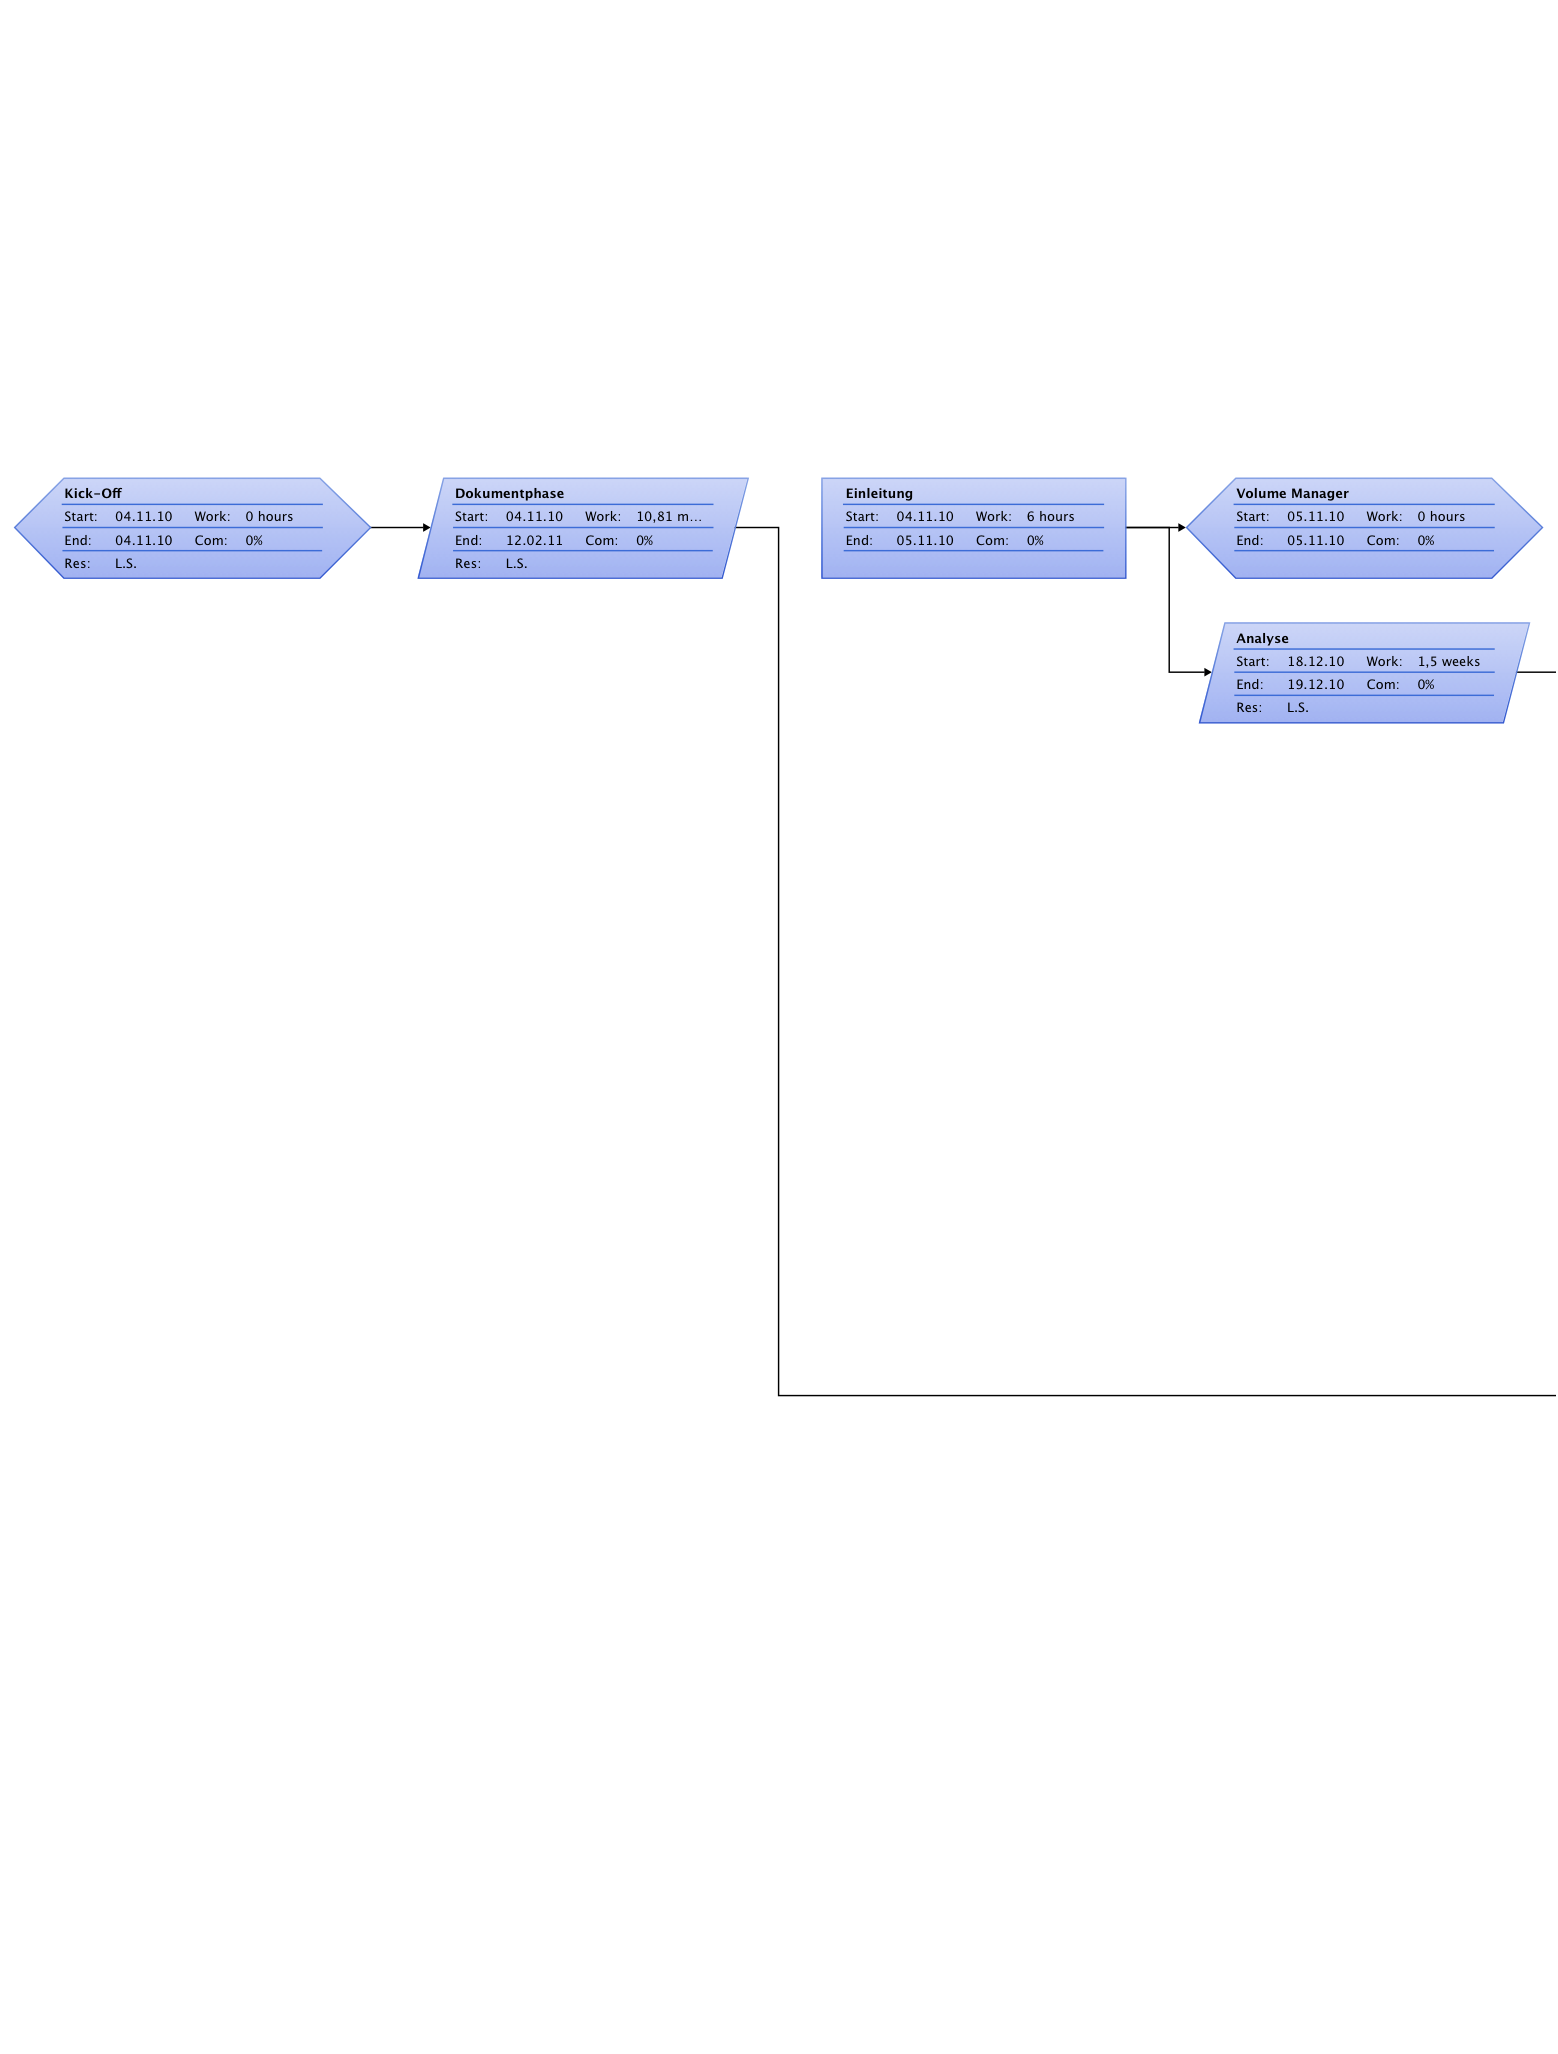
\includegraphics[width=1\textwidth ]{Netzplan2.png}
\caption{Projektplanung: Netzplan Teil 2}
\label{fig:Netzplan2}
\end{figure}

\begin{figure}[H]
\centering
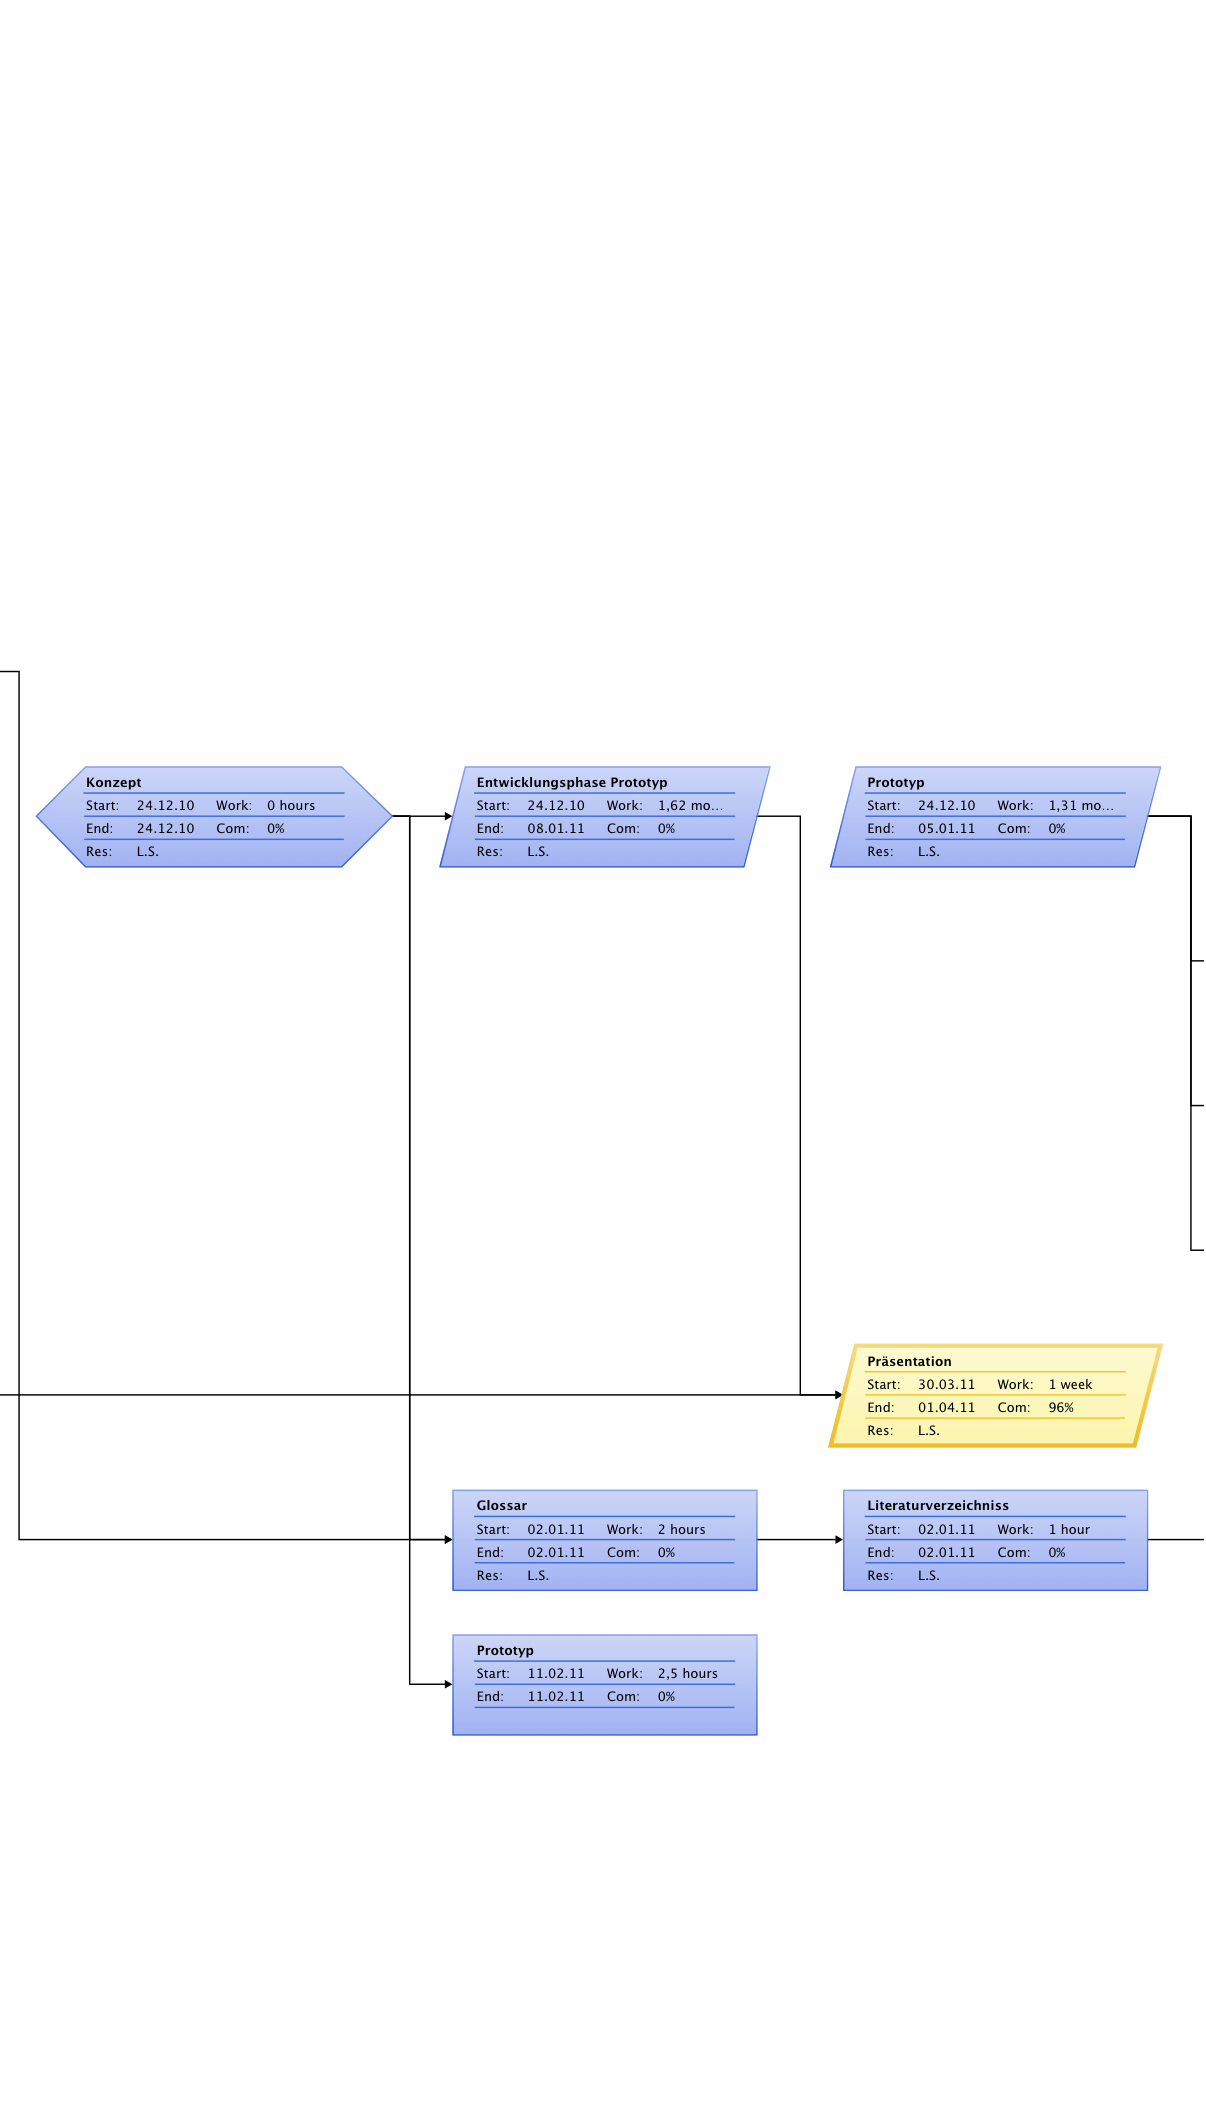
\includegraphics[width=1\textwidth]{Netzplan3.png}
\caption{Projektplanung: Netzplan Teil 3}
\label{fig:Netzplan3}
\end{figure}

\begin{figure}[H]
\centering
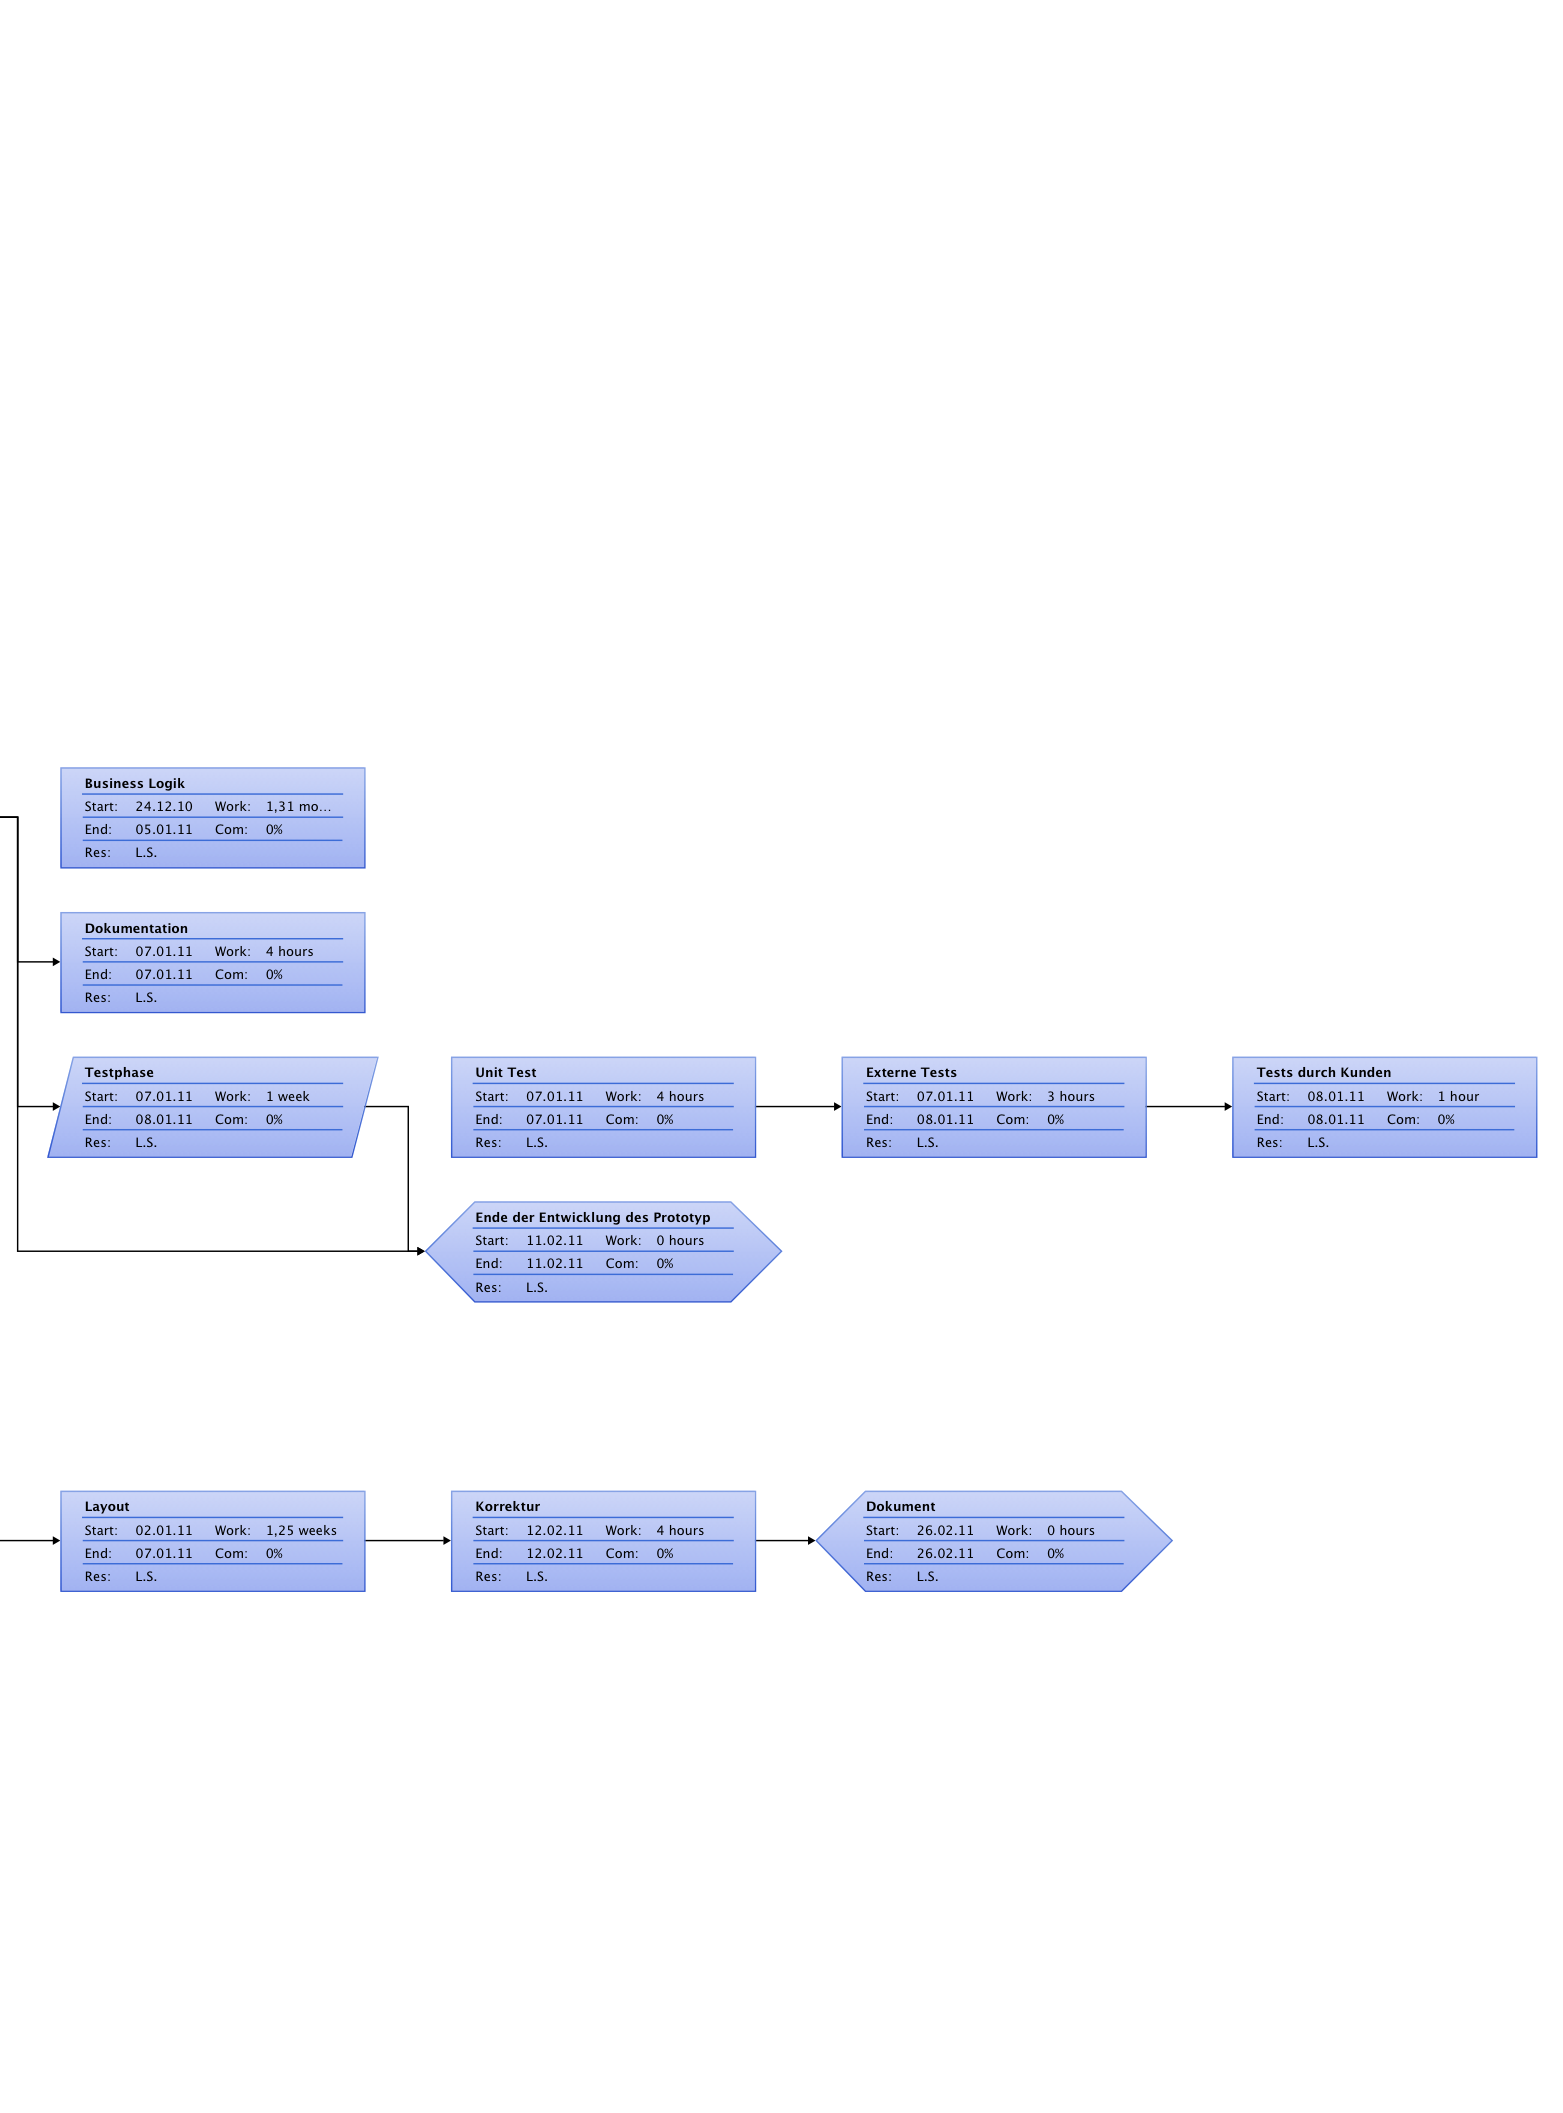
\includegraphics[width=1\textwidth]{Netzplan4.png}
\caption{Projektplanung: Netzplan Teil 4}
\label{fig:Netzplan4}
\end{figure}





 
    % Rand der Aufzählungen in Tabellen anpassen
    \setdefaultleftmargin{1em}{}{}{}{}{}
  %  
\section{Projektplanung}

\subsection{Meilensteine}

\begin{figure}[H]
\centering
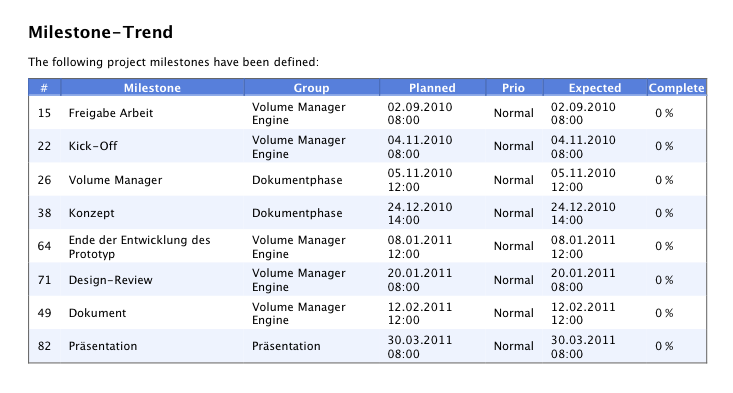
\includegraphics[width=1.2\textwidth]{Milestones.png}
\caption{Projektplanung: Meilensteine}
\label{fig:Meilensteine}
\end{figure}

\subsubsection{Trend}

\begin{figure}[H]
\centering
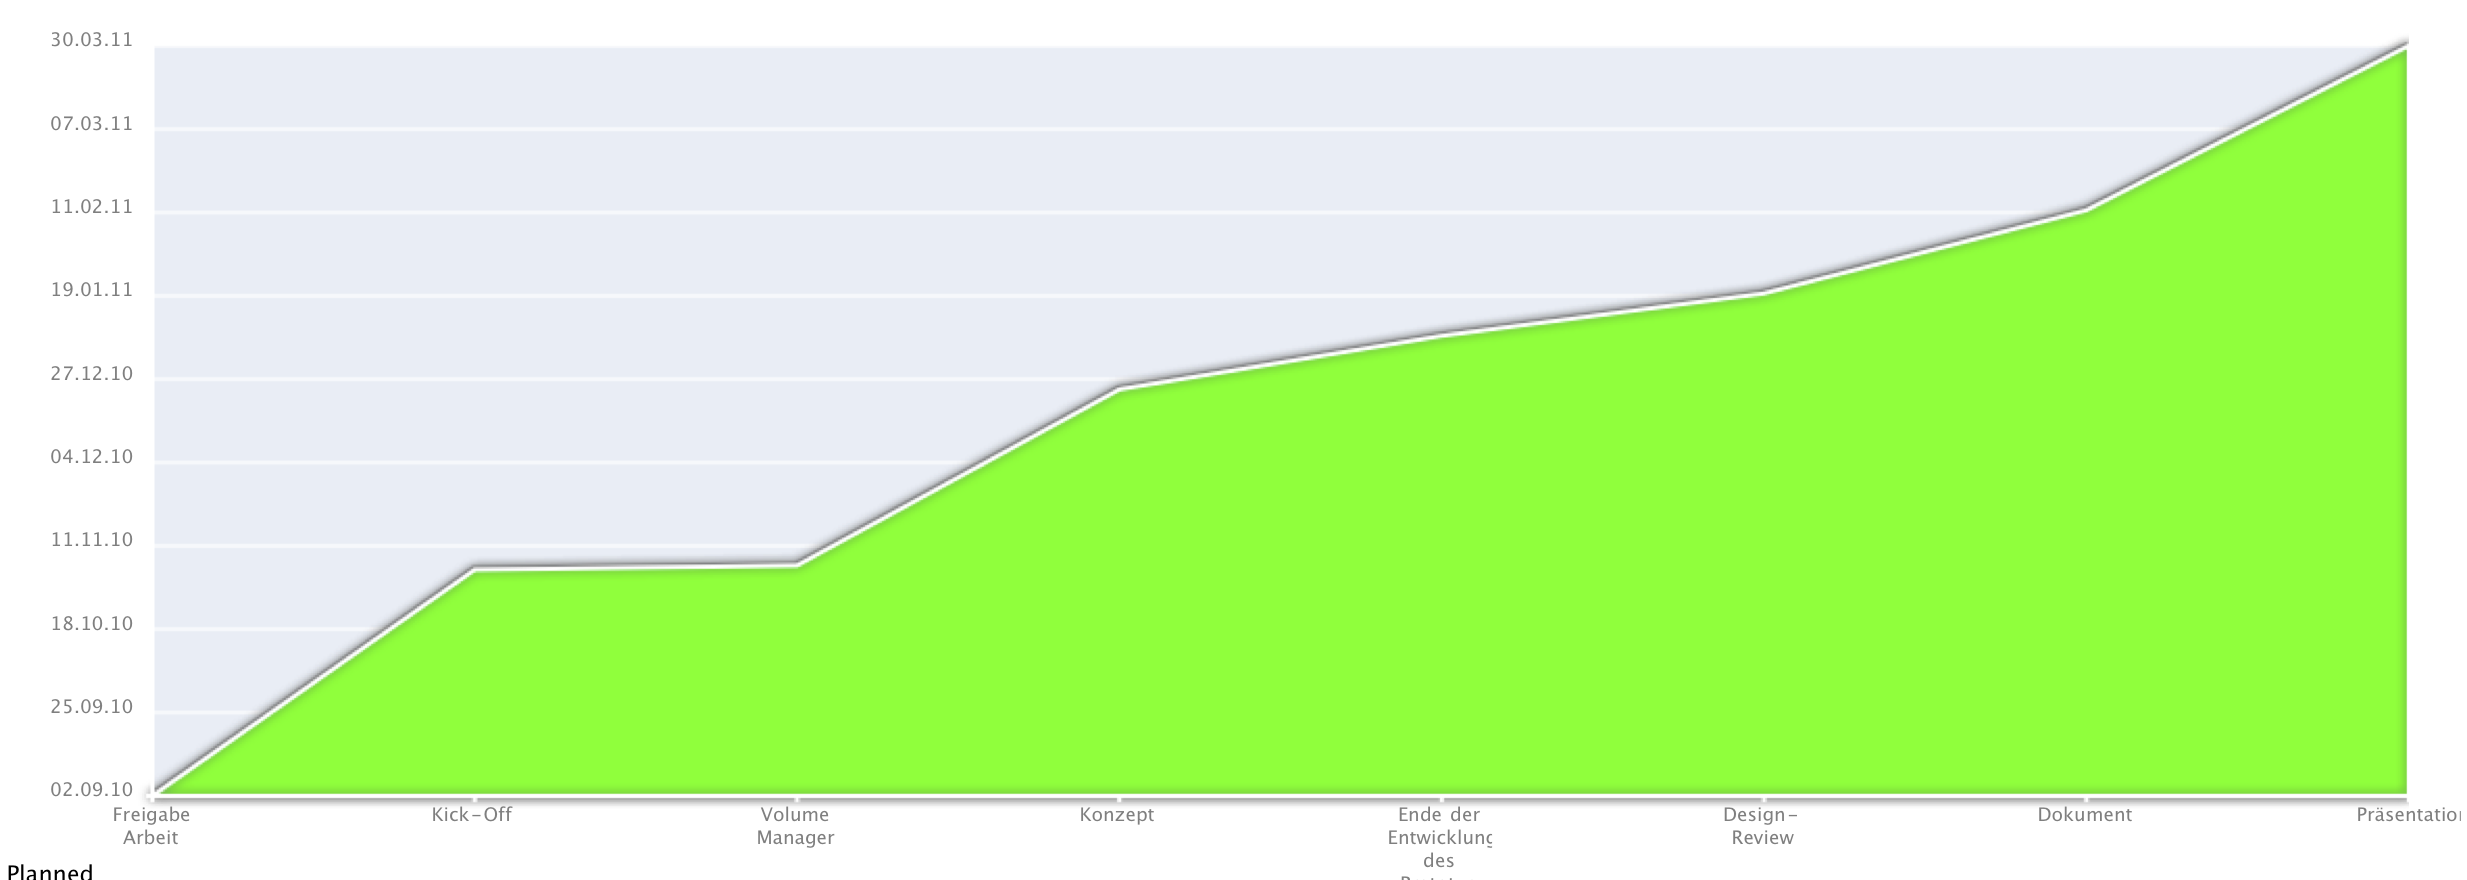
\includegraphics[width=1.4\textwidth, angle= 90]{MilestonesTrend.png}
\caption{Projektplanung: Meilensteine Trend}
\label{fig:MeilensteinTrend}
\end{figure}

\subsection{Netzplan}

\begin{figure}[H]
\centering
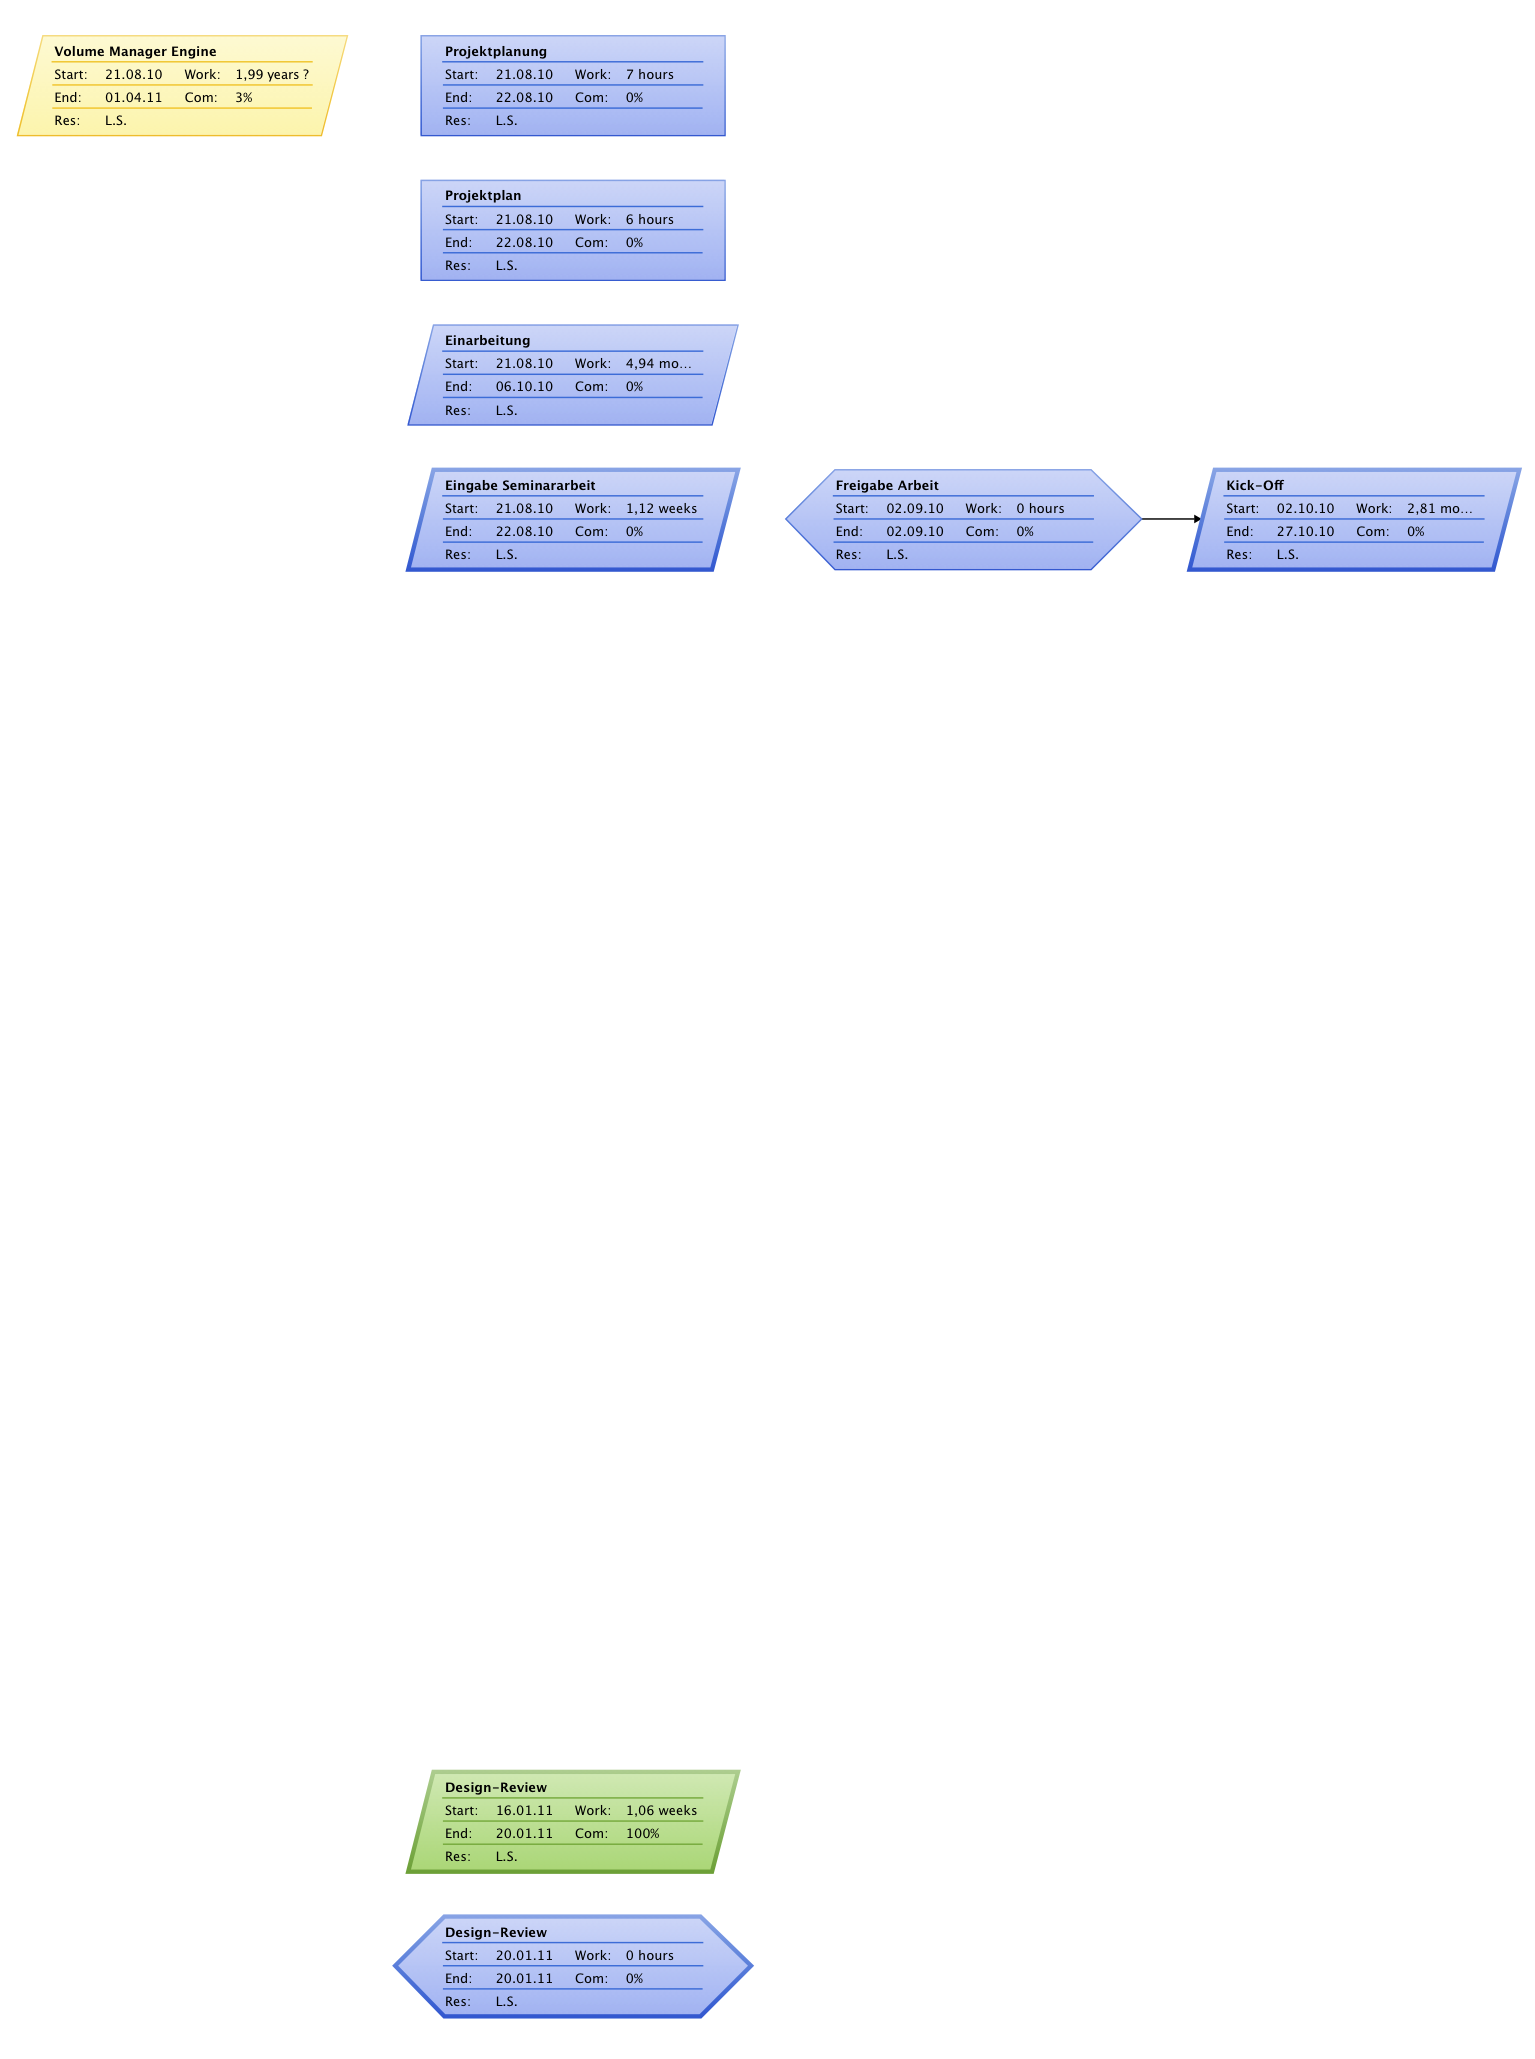
\includegraphics[width=1\textwidth]{Netzplan1.png}
\caption{Projektplanung: Netzplan Teil 1}
\label{fig:Netzplan1}
\end{figure}

\begin{figure}[H]
\centering
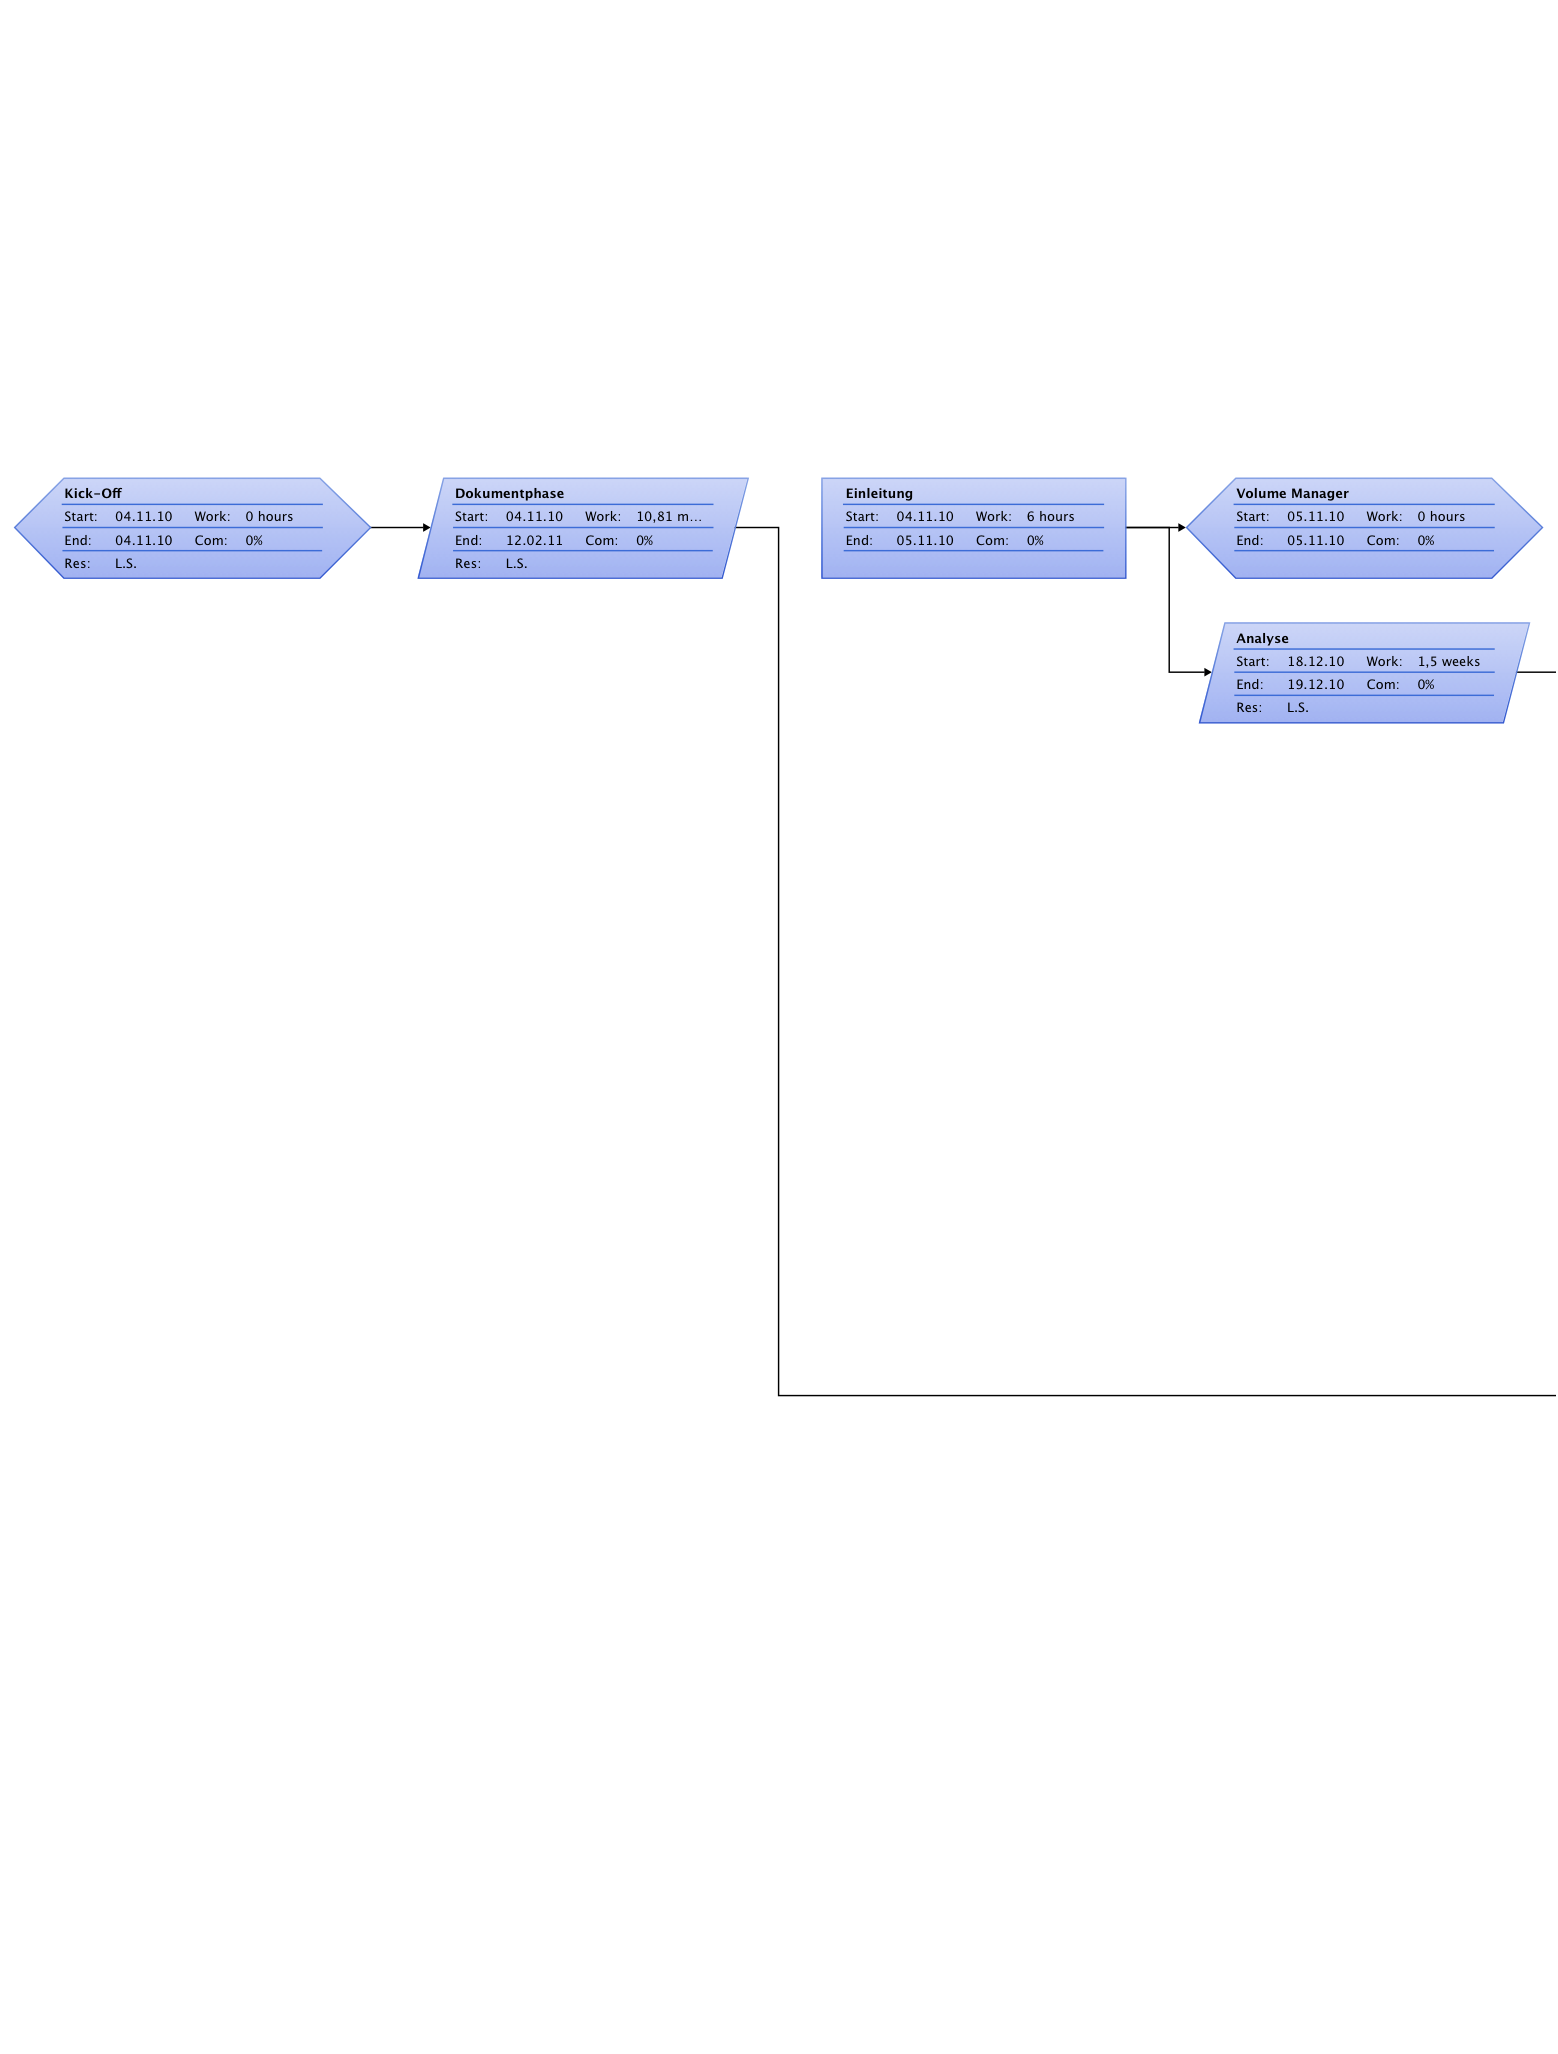
\includegraphics[width=1\textwidth ]{Netzplan2.png}
\caption{Projektplanung: Netzplan Teil 2}
\label{fig:Netzplan2}
\end{figure}

\begin{figure}[H]
\centering
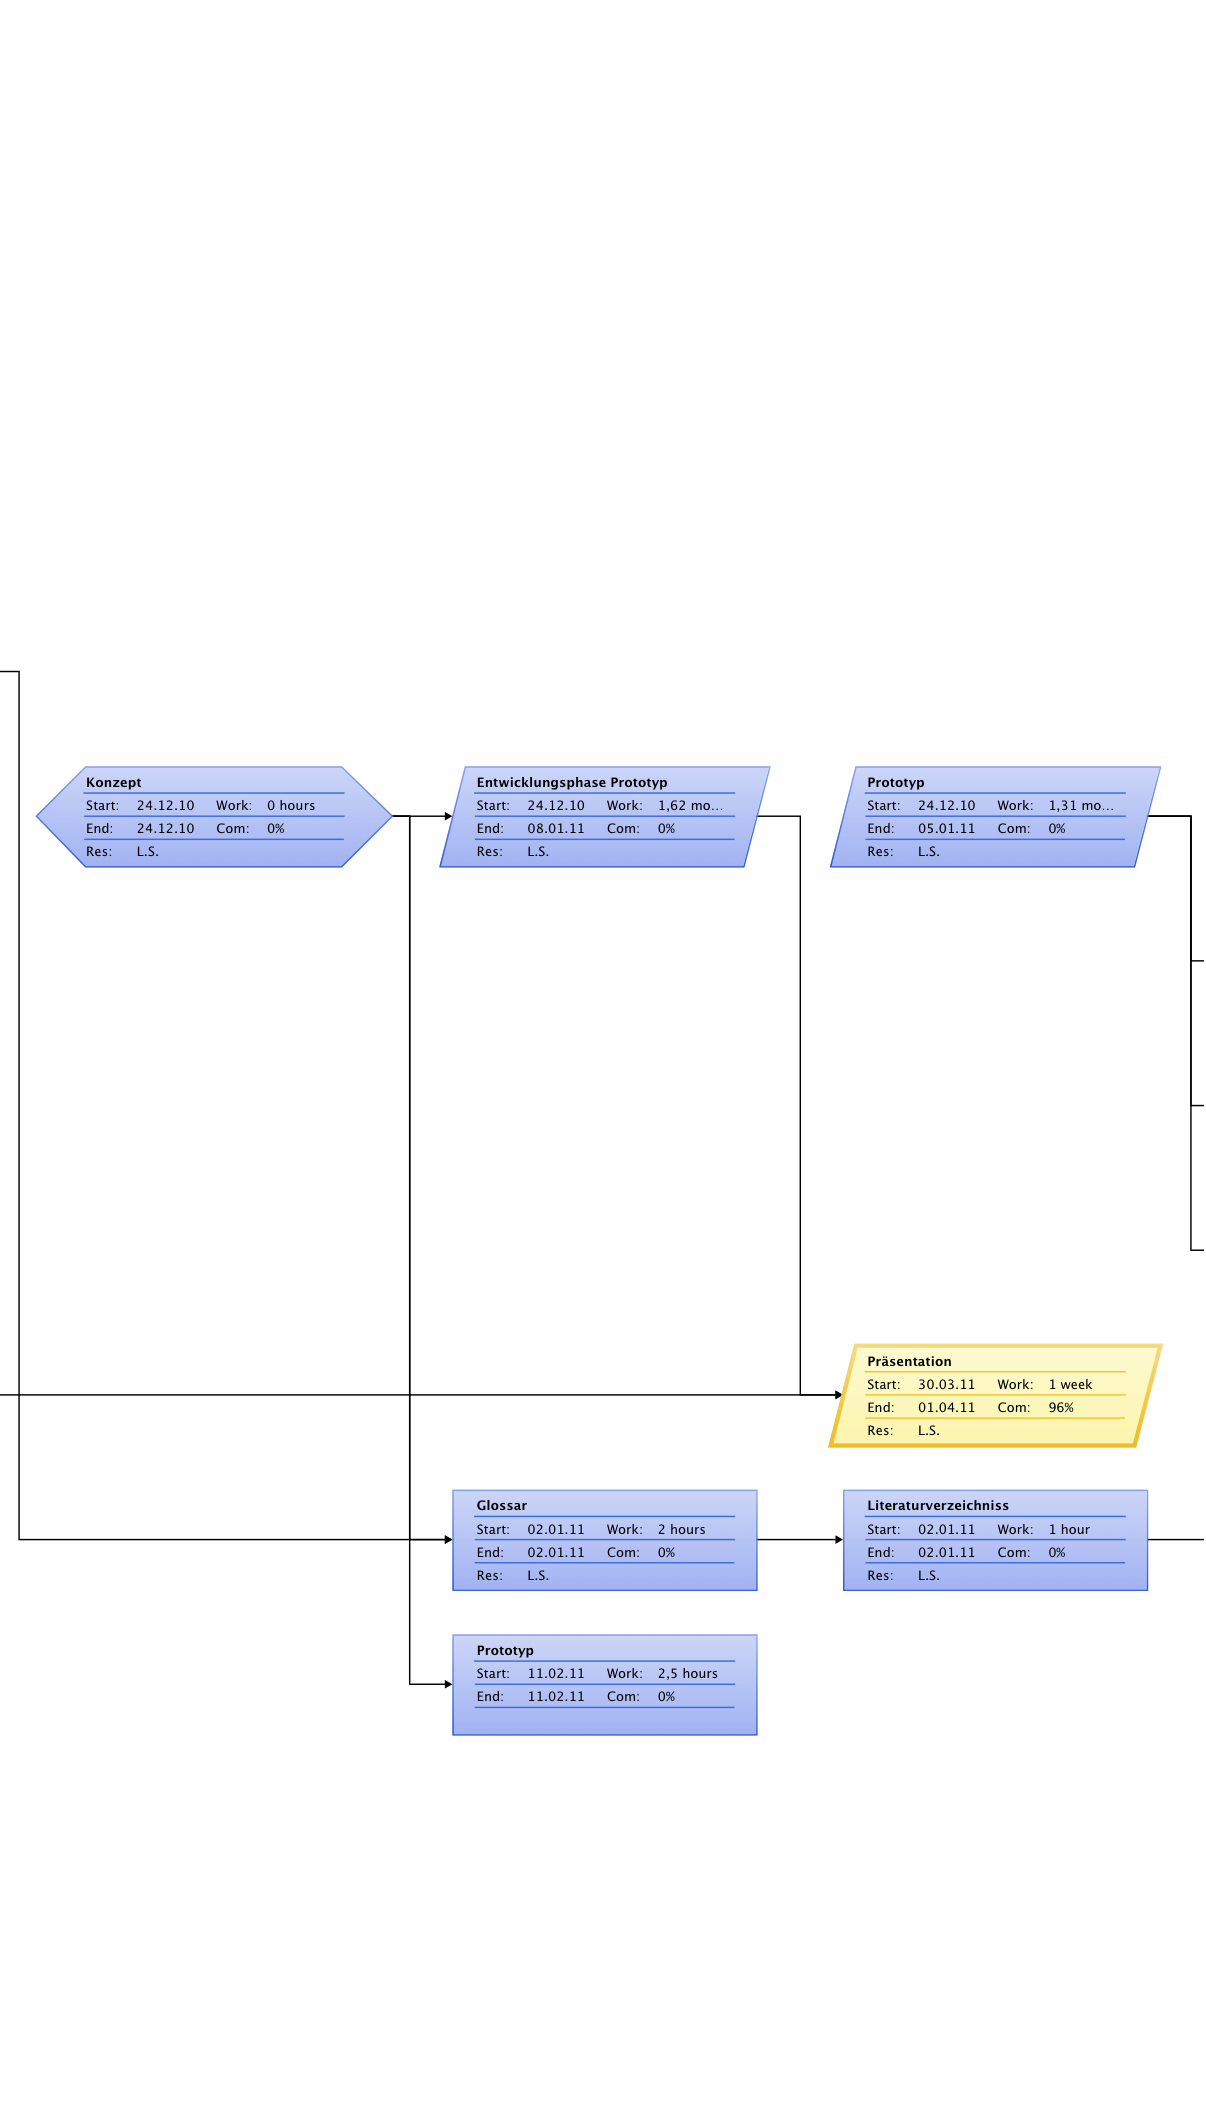
\includegraphics[width=1\textwidth]{Netzplan3.png}
\caption{Projektplanung: Netzplan Teil 3}
\label{fig:Netzplan3}
\end{figure}

\begin{figure}[H]
\centering
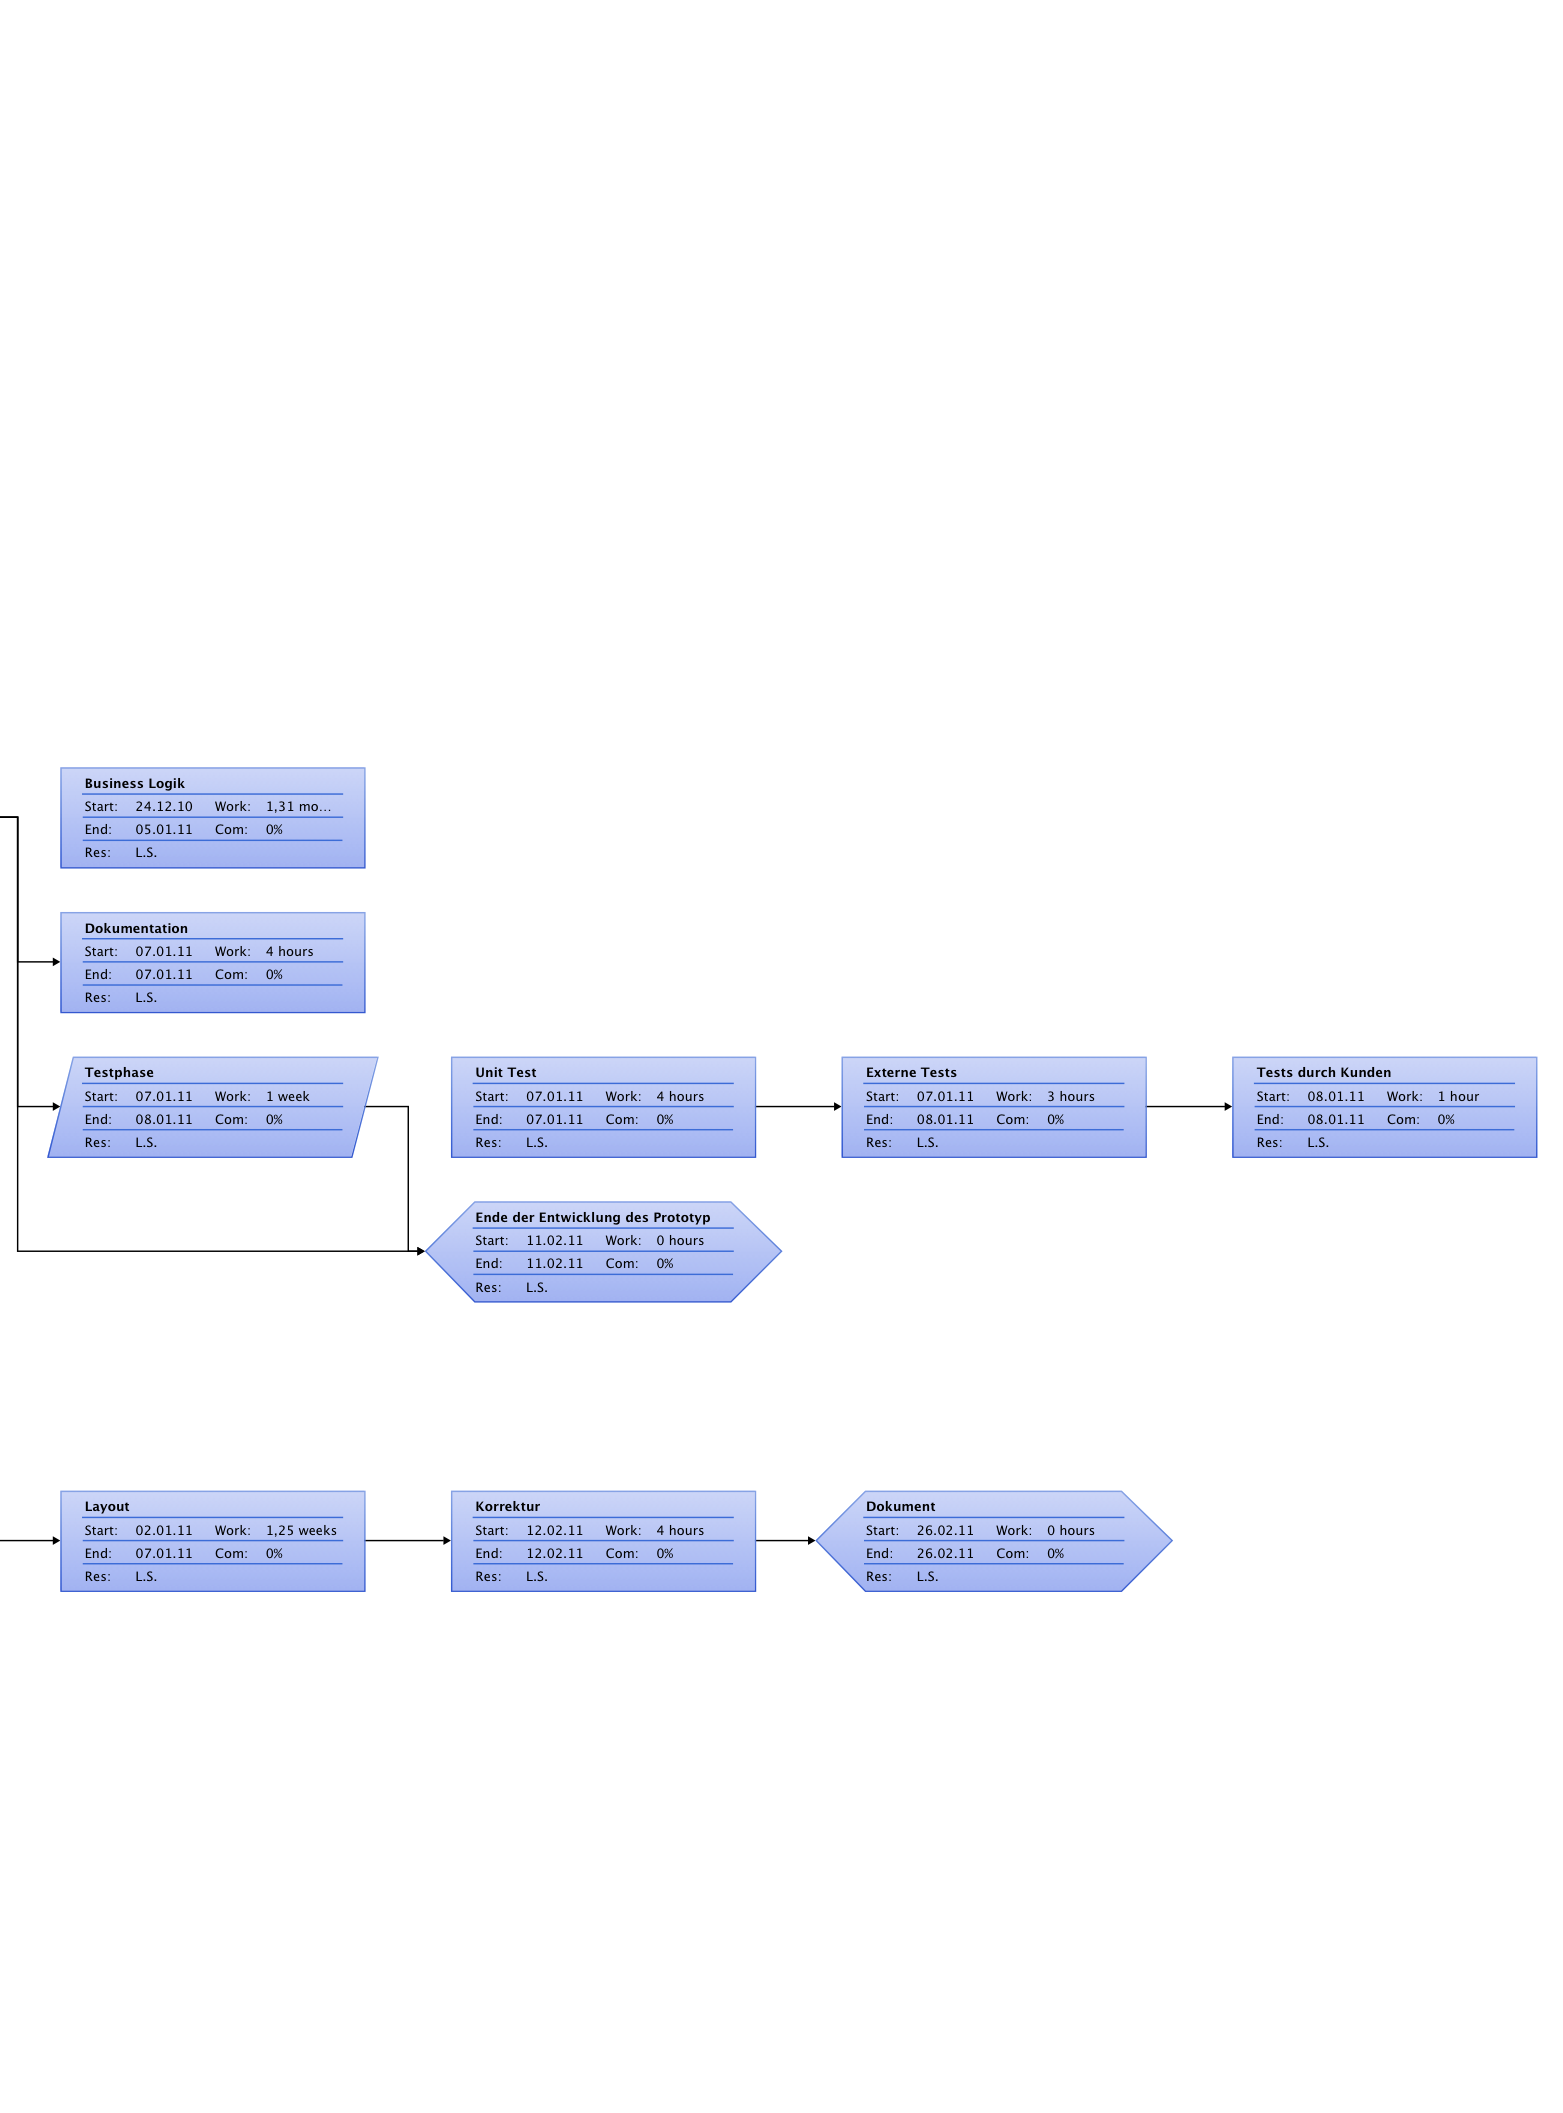
\includegraphics[width=1\textwidth]{Netzplan4.png}
\caption{Projektplanung: Netzplan Teil 4}
\label{fig:Netzplan4}
\end{figure}






\end{appendix}

% Index ------------------------------------------------------------------------
%   Zum Erstellen eines Index, die folgende Zeile auskommentieren.
% ------------------------------------------------------------------------------
%\printindex

\end{document}
